% 《时空与几何》中文重排本
% Sean M. Carroll, Spacetime and Geometry: An Introduction to General Relativity
% (Pearson New International Edition, 2014；内容同 Addison–Wesley 2004 第一版)
% 编译：xelatex ×3
\documentclass[11pt,a4paper,twoside,openright]{ctexbook}
\usepackage{amsmath,amssymb}
\usepackage{mathrsfs}
\usepackage[margin=2.4cm]{geometry}
\usepackage{graphicx}
\usepackage{float}
\usepackage{caption}
\usepackage{needspace}
\usepackage{booktabs}
\usepackage{multirow}
\usepackage{enumitem}
\ctexset{
  chapter/name = {第,章},
  section/format = \Large\bfseries,
}
\allowdisplaybreaks
\raggedbottom
\clubpenalty=10000 \widowpenalty=10000 \predisplaypenalty=10000
\graphicspath{{figures/}}
\xeCJKDeclareCharClass{CJK}{"201C, "201D, "2018, "2019}

% 插入的空白衬页真正空白（无页眉页脚）
\makeatletter
\def\cleardoublepage{\clearpage\if@twoside\ifodd\c@page\else
\hbox{}\thispagestyle{empty}\newpage\if@twocolumn\hbox{}\newpage\fi\fi\fi}
\makeatother

% 插图占位（翻译阶段先占位，图重绘后替换为 \includegraphics）
\newcommand{\figplaceholder}[2]{%
  \begin{figure}[H]\centering
  \fbox{\parbox[c][5cm][c]{0.8\textwidth}{\centering 图 #1 重绘占位\\ #2}}
  \caption*{图 #1\quad #2}\label{fig:auto:#1}
  \end{figure}}

% 章首题词（原书卷首引语）
\newcommand{\epigraphbook}[2]{%
  \begin{center}\itshape #1\\[0.3em]\scshape #2\end{center}}

\begin{document}
\frontmatter
\tableofcontents
 % 本文件由 scripts/assemble.py 自动装配，勿手改（改 parts/ 后重跑）
% 第8章 宇宙学

% 第8章 Cosmology
\chapter{宇宙学}

\section{最大对称宇宙}

% ---- 书页 323 / p338 ----
当代的宇宙学模型基于这样一种观念：宇宙在各处都大致相同——这一立场有时被称为\textbf{哥白尼原理}（Copernican principle）。乍一看，这种主张似乎很疯狂；比方说，太阳的中心与星际空间那荒凉的寒冷几乎毫无相似之处。但我们把哥白尼原理理解为仅仅适用在最大的尺度上，在那种尺度上密度的局域变化已被平均掉。它在这种尺度上的有效性体现在许多不同的观测之中，例如对星系的计数以及对弥漫 X 射线和 $\gamma$ 射线背景的观测；不过它最清晰的表现是 3K 的宇宙微波背景（cosmic microwave background，CMB）。虽然我们现在知道，微波背景辐射并非完美光滑（其实从来也没有人指望它完美光滑），但对规则性的偏离只有 $10^{-5}$ 的量级或更小，对于大尺度上时空的近似描述来说，这当然是足够好的基础。

哥白尼原理与流形可能具有的两个在数学上更精确的性质相关：各向同性（isotropy）与均匀性（homogeneity）。\textbf{各向同性}作用于流形中某个特定的点，它断言：无论你朝哪个方向看，空间看起来都一样。更正式地说，如果对于 $T_pM$ 中的任意两个矢量 $V$ 和 $W$，都存在 $M$ 的一个等距变换（isometry），使得 $W$ 在此等距变换下的推前与 $V$ 平行（$V$ 本身不被推前），那么流形 $M$ 就称为绕点 $p$ 各向同性。微波背景的观测所指示的，正是空间的各向同性。

\textbf{均匀性}则是度规在整个流形上都相同的陈述。换句话说，给定 $M$ 中任意两点 $p$ 和 $q$，都存在一个把 $p$ 变到 $q$ 的等距变换。注意，均匀性与各向同性之间没有必然的联系；一个流形可以均匀却无一处各向同性（比如通常度规下的 $\mathbf{R}\times S^2$），也可以绕某一点各向同性却不均匀（比如一个锥面，它绕自己的顶点各向同性，但显然不均匀）。另一方面，如果一个空间\emph{处处}各向同性，那么它就是均匀的。同样，如果它绕某一点各向同性并且还均匀，那么它将绕每一点都各向同性。既然各向同性有着充分的观测证据，而哥白尼原理又要我们相信自己并非宇宙的中心、因而别处的观者也应观测到各向同性，那么从今往后我们就同时假定均匀性和各向同性。

% ---- 书页 324 / p339 ----
均匀性和各向同性的用处在于，它们蕴含空间是最大对称的（maximally symmetric）。把各向同性想成转动下的不变性，把均匀性想成经过适当推广的平移下的不变性。于是均匀性和各向同性合在一起就蕴含：一个空间具有其可能的最大数目的 Killing 矢量。哥白尼原理的一个极端应用，是坚持认为时空本身就是最大对称的。事实上结果将表明并非如此；从观测上我们知道，宇宙在\emph{空间}上是均匀且各向同性的，但在全部\emph{时空}上却不是。不过，从考察最大对称的时空出发是有趣的（它们毕竟只是“仅空间最大对称”这一更普遍情形的特例）。我们将会看到，在某种意义上，这样的宇宙是广义相对论的“基态”。与本章后面的部分相比，这一讨论与观测到的宇宙关系较远；注重经验的读者不妨直接跳到下一节去。

我们在第 3 章中曾提到，带度规 $g_{\mu\nu}$ 的最大对称 $n$ 维流形，其 Riemann 张量可以写成
\begin{equation*}
R_{\rho\sigma\mu\nu} = \kappa\left(g_{\rho\mu}g_{\sigma\nu} - g_{\rho\nu}g_{\sigma\mu}\right),
\tag{8.1}
\end{equation*}
其中 $\kappa$ 是 Ricci 曲率的归一化量度，
\begin{equation*}
\kappa = \frac{R}{n(n-1)},
\tag{8.2}
\end{equation*}
而 Ricci 标量 $R$ 在流形上将是一个常数。由于在任何一个单点上我们总可以把度规化为规范形式（$g_{\mu\nu}=\eta_{\mu\nu}$），最大对称流形的种类在局域上就由度规的号差以及常数 $\kappa$ 的符号来刻画。需要“局域”这个限定词，是为了顾及可能的全局差异，比如平面与环面之间的差异。我们感兴趣的是号差为 $(-+++)$ 的度规。对于曲率为零（$\kappa=0$）的情形，最大对称时空是众所周知的；它恰恰就是 Minkowski 空间，其度规为
\begin{equation*}
\mathrm{d}s^2 = -\mathrm{d}t^2 + \mathrm{d}x^2 + \mathrm{d}y^2 + \mathrm{d}z^2.
\tag{8.3}
\end{equation*}
Minkowski 空间的共形图在附录 H 中导出。

曲率为正（$\kappa>0$）的最大对称时空称为 \textbf{de Sitter 空间}（de Sitter space）。考虑一个五维 Minkowski 空间，度规为 $\mathrm{d}s_5^2 = -\mathrm{d}u^2 + \mathrm{d}x^2 + \mathrm{d}y^2 + \mathrm{d}z^2 + \mathrm{d}w^2$，并在其中嵌入一个由下式给出的双曲面（hyperboloid）
\begin{equation*}
-u^2 + x^2 + y^2 + z^2 + w^2 = \alpha^2.
\tag{8.4}
\end{equation*}
现在按如下方式在双曲面上诱导坐标 $\{t,\chi,\theta,\phi\}$：
\begin{equation*}
\begin{aligned}
u &= \alpha\sinh(t/\alpha)\\
w &= \alpha\cosh(t/\alpha)\cos\chi\\
x &= \alpha\cosh(t/\alpha)\sin\chi\cos\theta\\
y &= \alpha\cosh(t/\alpha)\sin\chi\sin\theta\cos\phi\\
z &= \alpha\cosh(t/\alpha)\sin\chi\sin\theta\sin\phi.
\end{aligned}
\tag{8.5}
\end{equation*}
% ---- 书页 325 / p340 ----（原书 324/325 分页恰落在本式内：(u,w) 在书页 324，(x,y,z) 及其后文字在书页 325；两块已按原书合并为单个五行公式） ----
于是双曲面上的度规为
\begin{equation*}
\mathrm{d}s^2 = -\mathrm{d}t^2 + \alpha^2\cosh^2(t/\alpha)\left[\mathrm{d}\chi^2 + \sin^2\chi\left(\mathrm{d}\theta^2 + \sin^2\theta\,\mathrm{d}\phi^2\right)\right].
\tag{8.6}
\end{equation*}
我们认出圆括号中的表达式是二维球面上的度规 $\mathrm{d}\Omega_2^2$，而方括号中的表达式是三维球面上的度规 $\mathrm{d}\Omega_3^2$。这样，de Sitter 空间描述的是一个先是收缩、在 $t=0$ 时达到最小尺寸、然后再重新膨胀的空间三维球面。当然，这一特殊描述承袭自某个特定的坐标系；我们将看到，同样有效的其他描述也是存在的。

这些坐标覆盖整个流形。一般你可以这样检验这一点：比如追踪测地线在坐标系边缘附近的行为；如果坐标不完备，测地线看起来就会在有限的仿射参量处终止。因此 de Sitter 空间的拓扑是 $\mathbf{R}\times S^3$。这使得导出共形图变得非常简单，因为构造共形图的关键一步，就是把度规写成它与 Einstein 静态宇宙（一个拓扑为 $\mathbf{R}\times S^3$、描述一个随时间推移保持半径不变的空间三维球面的时空）共形相关联的形式。考虑从 $t$ 到 $t'$ 的坐标变换
\begin{equation*}
\cosh(t/\alpha) = \frac{1}{\cos(t')}.
\tag{8.7}
\end{equation*}
度规 (8.6) 于是变为
\begin{equation*}
\mathrm{d}s^2 = \frac{\alpha^2}{\cos^2(t')}\,\mathrm{d}\bar{s}^2,
\tag{8.8}
\end{equation*}
其中 $\mathrm{d}\bar{s}^2$ 表示 Einstein 静态宇宙上的度规，
\begin{equation*}
\mathrm{d}\bar{s}^2 = -(\mathrm{d}t')^2 + \mathrm{d}\chi^2 + \sin^2\chi\,\mathrm{d}\Omega_2^2.
\tag{8.9}
\end{equation*}
新时间坐标的范围是
\begin{equation*}
-\pi/2 < t' < \pi/2.
\tag{8.10}
\end{equation*}
de Sitter 空间的共形图就是与 de Sitter 共形相关的那一片 Einstein 静态宇宙区域的表示。它看起来像一个正方形，如图 8.1 所示。常数 $t'$ 的类空切片代表一个三维球面；左右两条边缘处的虚线是这个球面的北极和南极。对角线代表类光射线；在过去无限远释放的一个光子，恰好会在未来无限远时到达球面上正对面的那一点（对跖点）。

\begin{figure}[H]
\centering
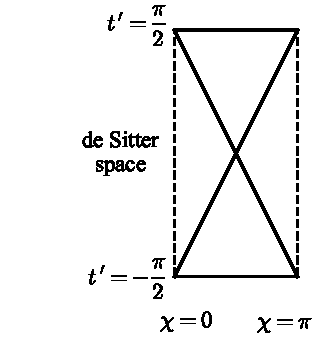
\includegraphics[width=0.72\textwidth]{fig_8.1.pdf}
\caption*{图 8.1\quad de Sitter 时空的共形图。类空切片是三维球面，因此图上的点代表二维球面，只有左右两条边缘上的点除外——它们代表单个点。}
\end{figure}

% ---- 书页 326 / p341 ----
请记住，时空之所以向过去和未来“终结”，仅仅是共形变换的魔力所致；真实的 de Sitter 空间向未来和过去无限延伸。还要注意，两个点可以拥有完全断开的未来（或过去）光锥；这反映了这样一个事实：球状空间截面膨胀得如此之快，以至于来自一点的光永远无法与来自另一点的光相接触。

一个类似的双曲面构造揭示了最大对称而 $\kappa<0$ 的时空，即所谓的 \textbf{反 de Sitter 空间}（anti-de Sitter space）。从一个虚构的五维平直流形出发，其度规为 $\mathrm{d}s_5^2 = -\mathrm{d}u^2 - \mathrm{d}v^2 + \mathrm{d}x^2 + \mathrm{d}y^2 + \mathrm{d}z^2$，并嵌入一个由下式给出的双曲面
\begin{equation*}
-u^2 - v^2 + x^2 + y^2 + z^2 = -\alpha^2.
\tag{8.11}
\end{equation*}
注意这里所有的负号。然后我们可以在双曲面上诱导坐标 $\{t',\rho,\theta,\phi\}$：
\begin{equation*}
\begin{aligned}
u &= \alpha\sin(t')\cosh(\rho)\\
v &= \alpha\cos(t')\cosh(\rho)\\
x &= \alpha\sinh(\rho)\cos\theta\\
y &= \alpha\sinh(\rho)\sin\theta\cos\phi\\
z &= \alpha\sinh(\rho)\sin\theta\sin\phi,
\end{aligned}
\tag{8.12}
\end{equation*}
由此得到这个双曲面上如下形式的度规：
\begin{equation*}
\mathrm{d}s^2 = \alpha^2\left(-\cosh^2(\rho)\,\mathrm{d}t'^2 + \mathrm{d}\rho^2 + \sinh^2(\rho)\,\mathrm{d}\Omega_2^2\right).
\tag{8.13}
\end{equation*}
这些坐标有一个奇怪的特点，即 $t'$ 是周期的。由 (8.12)，$t'$ 与 $t'+2\pi$ 代表双曲面上的同一个位置。由于 $\partial_{t'}$ 处处类时，当 $t'$ 增加时保持 $\{\rho,\theta,\phi\}$ 不变的曲线将是一条闭合类时曲线。然而，这并不是时空的内禀性质，只是我们从特定嵌入导出度规的方式所带来的假象。我们完全可以转而考虑这个流形的“覆盖空间”（covering space），即度规由 (8.13) 给出、但允许 $t'$ 从 $-\infty$ 变到 $\infty$ 的时空。这个空间中没有闭合类时曲线，我们就把这一点取作反 de Sitter 空间的定义。

为了导出共形图，进行一个与 de Sitter 情形类似的坐标变换，不过这次作用在径向坐标上：
\begin{equation*}
\cosh(\rho) = \frac{1}{\cos\chi},
\tag{8.14}
\end{equation*}
于是
\begin{equation*}
\mathrm{d}s^2 = \frac{\alpha^2}{\cos^2\chi}\,\mathrm{d}\bar{s}^2,
\tag{8.15}
\end{equation*}

% ---- 书页 327 / p342 ----
\begin{figure}[H]
\centering
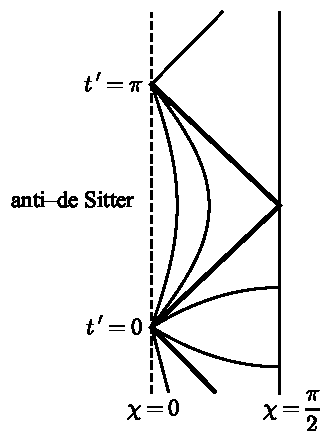
\includegraphics[width=0.72\textwidth]{fig_8.2.pdf}
\caption*{图 8.2\quad 反 de Sitter 时空的共形图。类空切片具有 $\mathbf{R}^3$ 的拓扑，我们用极坐标把它表示出来，因此图上的点代表二维球面，只有左边的点除外——它们代表空间原点处的单个点。无限远是右侧的一个类时曲面。}
\end{figure}

其中 $\mathrm{d}\bar{s}^2$ 表示 Einstein 静态宇宙的度规 (8.9)。与 de Sitter 不同，径向坐标现在出现在共形因子之中。此外，对反 de Sitter 而言，$t'$ 坐标从负无穷一直到正无穷，而径向坐标的范围是
\begin{equation*}
0 \leq \chi < \frac{\pi}{2}.
\tag{8.16}
\end{equation*}
这样，反 de Sitter 空间与 Einstein 静态宇宙的一半共形相关联。其共形图示于图 8.2，图中画出了几条通过点 $t'=0$、$\chi=0$ 的有代表性的类时和类空测地线。由于 $\chi$ 只到 $\pi/2$ 而不是一直到 $\pi$，这个时空的类空切片具有 $S^3$ 中一个半球面内部的拓扑；也就是说，它在拓扑上是 $\mathbf{R}^3$（因而整个时空具有拓扑 $\mathbf{R}^4$）。注意，我们用极坐标画出这张图：左边的一点代表空间原点处的一个点，而右边的一点代表空间无限远处的一个二维球面。另一种流行的表示方法是画出时空的横截面，让空间原点位于正中间，而右边和左边合起来构成空间无限远。

反 de Sitter 的一个有趣特点是，无限远以一个类时超曲面的形式出现，由 $\chi=\pi/2$ 定义。由于无限远是类时的，这个空间不是全局双曲的，我们就没有一个以类空切片上给定的信息来表述的适定初值问题，因为信息总是可以“从无穷远流入”。另一个有趣的特点是，指数映射并不映满整个时空；如图中所画的那样，从指定点出发的测地线并不覆盖整个流形。指向未来的类时测地线，如图所示，起初可以从 $t'=0$、$\chi=0$ 沿径向向外运动，但最终会重新聚焦到点 $t'=\pi$、$\chi=0$，然后再次沿径向向外运动。

% ---- 书页 328 / p343 ----
顺便说一句，我们忍不住要指出：无限远的类时性质促成了弦论的一个引人注目的特征——“AdS/CFT 对应”（AdS/CFT correspondence）。这里 AdS 当然就是我们一直在讨论的反 de Sitter 空间，而 CFT 指的是定义在边界上的共形不变的场论［对 $n$ 维 AdS 来说，这个边界本身就是一个 $(n-1)$ 维时空］。AdS/CFT 对应表明，在某个极限下，AdS 背景上的量子引力（或其超对称版本）与定义在边界上的共形不变的非引力场论之间存在等价关系。关于非引力的量子场论我们知道得很多，而对量子引力却知之甚少，因此这一对应（如果它是正确的——这看起来很有可能，但尚未被证明）将揭示量子引力中可能发生之事的大量信息。\footnote{全面的综述文章见 O.~Aharony, S.S.~Gubser, J.M.~Maldacena, H.~Ooguri, and Y.~Oz, \emph{Phys.\ Rept.} \textbf{323}, 183 (2000), \texttt{http://arxiv.org/hep-th/9905111}。}

于是我们有了三个最大对称的时空：Minkowski（$\kappa=0$）、de Sitter（$\kappa>0$）和反 de Sitter（$\kappa<0$）。它们中有哪一个是真实世界的有用模型吗？进而言之，它们是 Einstein 方程的解吗？先对 (8.1) 给出的 Riemann 张量取迹，并限定到四维：
\begin{equation*}
R_{\mu\nu} = 3\kappa g_{\mu\nu},\qquad R = 12\kappa.
\tag{8.17}
\end{equation*}
可见在最大对称空间中，Ricci 张量与度规成正比。具有这种性质的时空有时被称为 Einstein 空间（Einstein space）；而 Einstein 静态宇宙并\emph{不}是 Einstein 空间的一个例子，这一点有时会令人混淆。更糟的是，我们后面还会遇到 Einstein–de Sitter 宇宙学，它既与 Einstein 空间无关，也与 Einstein 静态宇宙或 de Sitter 空间无关。Einstein 张量为
\begin{equation*}
G_{\mu\nu} = R_{\mu\nu} - \frac{1}{2}Rg_{\mu\nu} = -3\kappa g_{\mu\nu}.
\tag{8.18}
\end{equation*}
因此，Einstein 方程 $G_{\mu\nu}=8\pi G T_{\mu\nu}$ 蕴含（在最大对称时空中如此，并非普遍情形）能量-动量张量与度规成正比：
\begin{equation*}
T_{\mu\nu} = -\frac{3\kappa}{8\pi G}\,g_{\mu\nu}.
\tag{8.19}
\end{equation*}
这样的能量-动量张量对应于真空能或宇宙学常数，如第 4 章所讨论的。能量密度和压强为
\begin{equation*}
\rho = -p = \frac{3\kappa}{8\pi G}.
\tag{8.20}
\end{equation*}
若 $\rho$ 为正，我们得到 de Sitter 解；若 $\rho$ 为负，我们得到反 de Sitter。但在我们的宇宙中，除了可能有真空能之外，还有普通的物质和辐射。我们的最大对称时空并不相容于
% ---- 书页 329 / p344 ----
动力学上可观的物质和/或辐射。此外，由于我们观测到宇宙中的可见物质正在彼此分开（宇宙正在膨胀，下面会讨论），物质的密度在过去更高；所以即使物质对总能量的贡献在今天可以忽略，它在更早的宇宙中也曾经是可观的。因此，最大对称时空并不是真实世界的合理模型。不过，它们确实代表了在没有任何普通物质或引力辐射时 Einstein 方程的（局域）唯一解；正是在这个意义上，它们可以被看作广义相对论的基态。

\section{Robertson–Walker 度规}

为了描述真实世界，我们不得不放弃“完美的”哥白尼原理——它蕴含空间和时间处处都对称——而假定某种更宽容的东西。事实证明，直接假定宇宙在\emph{空间上}均匀且各向同性、但随时间演化，既是直截了当的，又与观测一致。在广义相对论中，这转译为如下陈述：宇宙可以叶状分层（foliated）为一些类空切片，使得每个三维切片都是最大对称的。于是我们把时空取为 $\mathbf{R}\times\Sigma$，其中 $\mathbf{R}$ 代表时间方向，而 $\Sigma$ 是一个最大对称的三维流形。时空度规因此取如下形式
\begin{equation*}
\mathrm{d}s^2 = -\mathrm{d}t^2 + R^2(t)\,\mathrm{d}\sigma^2,
\tag{8.21}
\end{equation*}
其中 $t$ 是类时坐标，$R(t)$ 是一个称为\textbf{尺度因子}（scale factor）的函数，而 $\mathrm{d}\sigma^2$ 是 $\Sigma$ 上的度规，它可以表示为
\begin{equation*}
\mathrm{d}\sigma^2 = \gamma_{ij}(u)\,\mathrm{d}u^i\,\mathrm{d}u^j,
\tag{8.22}
\end{equation*}
其中 $(u^1,u^2,u^3)$ 是 $\Sigma$ 上的坐标，$\gamma_{ij}$ 是一个最大对称的三维度规。尺度因子告诉我们类空切片 $\Sigma$ 在时刻 $t$ 有多大。（不要把它与标量曲率混淆。）这里使用的坐标，其度规没有交叉项 $\mathrm{d}t\,\mathrm{d}u^i$，且 $\mathrm{d}t^2$ 的系数与 $u^i$ 无关，称为\textbf{共动坐标}（comoving coordinates），它是附录 D 讨论的高斯法坐标的一个特例。保持在常数 $u^i$ 处的观者也称为“共动的”。只有共动观者才会认为宇宙看起来是各向同性的；事实上在地球上我们并不完全共动，结果便是我们在宇宙微波背景中看到偶极各向异性，它来源于常规的多普勒效应。

因此我们感兴趣的是最大对称的欧几里得三维度规 $\gamma_{ij}$。我们知道，最大对称的度规满足
\begin{equation*}
{}^{(3)}R_{ijkl} = k\left(\gamma_{ik}\gamma_{jl} - \gamma_{il}\gamma_{jk}\right),
\tag{8.23}
\end{equation*}
其中为了今后的方便我们引入了
\begin{equation*}
k = {}^{(3)}R/6,
\tag{8.24}
\end{equation*}

% ---- 书页 330 / p345 ----
并且在 Riemann 张量上放一个上标 $(3)$，提醒我们它与三维度规 $\gamma_{ij}$ 相联系，而不是与整个时空的度规相联系。Ricci 张量便是
\begin{equation*}
{}^{(3)}R_{jl} = 2k\gamma_{jl}.
\tag{8.25}
\end{equation*}
如果空间要是最大对称的，那它肯定是球对称的。从对 Schwarzschild 解的探索中，我们已经对球对称空间有所了解；度规可以写成
\begin{equation*}
\mathrm{d}\sigma^2 = \gamma_{ij}\,\mathrm{d}u^i\,\mathrm{d}u^j = e^{2\beta(\bar{r})}\,\mathrm{d}\bar{r}^2 + \bar{r}^2\,\mathrm{d}\Omega^2,
\tag{8.26}
\end{equation*}
其中 $\bar{r}$ 是径向坐标，二维球面上的度规一如既往是 $\mathrm{d}\Omega^2 = \mathrm{d}\theta^2 + \sin^2\theta\,\mathrm{d}\phi^2$。这种度规的 Ricci 张量分量可以从 (5.14)——静态球对称时空的 Ricci 张量——通过令 $\alpha=0$ 和 $r=\bar{r}$ 得到，即
\begin{equation*}
\begin{aligned}
{}^{(3)}R_{11} &= \frac{2}{\bar{r}}\,\partial_1\beta\\
{}^{(3)}R_{22} &= e^{-2\beta}\left(\bar{r}\,\partial_1\beta - 1\right) + 1\\
{}^{(3)}R_{33} &= \left[e^{-2\beta}\left(\bar{r}\,\partial_1\beta - 1\right) + 1\right]\sin^2\theta.
\end{aligned}
\tag{8.27}
\end{equation*}
我们利用 (8.25) 令它们与度规成正比，就可以解出 $\beta(\bar{r})$：
\begin{equation*}
\beta = -\frac{1}{2}\ln\left(1-k\bar{r}^2\right),
\tag{8.28}
\end{equation*}
由此得到三维曲面 $\Sigma$ 上的度规
\begin{equation*}
\mathrm{d}\sigma^2 = \frac{\mathrm{d}\bar{r}^2}{1-k\bar{r}^2} + \bar{r}^2\,\mathrm{d}\Omega^2.
\tag{8.29}
\end{equation*}
从 (8.24) 可以注意到，$k$ 的值决定了空间曲面的曲率，从而决定了空间曲面的大小。通常把它归一化，使得
\begin{equation*}
k \in \{+1, 0, -1\},
\tag{8.30}
\end{equation*}
而把流形的物理尺寸吸收进尺度因子 $R(t)$。

$k=-1$ 的情形对应于 $\Sigma$ 上曲率为负的常数，有时称为\textbf{开放}（open）；$k=0$ 的情形对应于 $\Sigma$ 上没有曲率，称为\textbf{平直}（flat）；$k=+1$ 的情形对应于 $\Sigma$ 上曲率为正，有时称为\textbf{闭合}（closed）。引入一个由下式定义的新径向坐标 $\chi$，得到度规的另一种形式，可以使这些情形的物理解释更加清楚：
\begin{equation*}
\mathrm{d}\chi = \frac{\mathrm{d}\bar{r}}{\sqrt{1-k\bar{r}^2}}.
\tag{8.31}
\end{equation*}

% ---- 书页 331 / p346 ----
这可以积分得到
\begin{equation*}
\bar{r} = S_k(\chi),
\tag{8.32}
\end{equation*}
其中
\begin{equation*}
S_k(\chi) \equiv
\begin{cases}
\sin(\chi), & k = +1\\
\chi, & k = 0\\
\sinh(\chi), & k = -1,
\end{cases}
\tag{8.33}
\end{equation*}
于是
\begin{equation*}
\mathrm{d}\sigma^2 = \mathrm{d}\chi^2 + {S_k}^2(\chi)\,\mathrm{d}\Omega^2.
\tag{8.34}
\end{equation*}
对平直情形 $k=0$，$\Sigma$ 上的度规变为
\begin{equation*}
\begin{aligned}
\mathrm{d}\sigma^2 &= \mathrm{d}\chi^2 + \chi^2\,\mathrm{d}\Omega^2\\
&= \mathrm{d}x^2 + \mathrm{d}y^2 + \mathrm{d}z^2,
\end{aligned}
\tag{8.35}
\end{equation*}
这就是平直的欧几里得空间。整体上，它可以描述 $\mathbf{R}^3$ 或者更复杂的流形，比如三维环面 $S^1\times S^1\times S^1$。对闭合情形 $k=+1$，我们有
\begin{equation*}
\mathrm{d}\sigma^2 = \mathrm{d}\chi^2 + \sin^2\chi\,\mathrm{d}\Omega^2,
\tag{8.36}
\end{equation*}
这是三维球面的度规。在这种情形下，唯一可能的整体结构是完全的三维球面（不可定向流形 $\mathbf{RP}^3$ 除外，它由认同 $S^3$ 上的对跖点得到）。最后，对开放的 $k=-1$ 情形，我们得到
\begin{equation*}
\mathrm{d}\sigma^2 = \mathrm{d}\chi^2 + \sinh^2\chi\,\mathrm{d}\Omega^2.
\tag{8.37}
\end{equation*}
这是常负曲率三维空间的度规，是 3.9 节讨论的那个双曲面的推广。整体上，这样的空间可以无限延伸（这正是“开放”一词的由来），但它也可以描述一个非单连通的紧致空间（所以“开放”实在算不上最准确的描述）。

时空的度规描述的正是这些最大对称超曲面之一在尺寸上的演化，它可以写成
\begin{equation*}
\mathrm{d}s^2 = -\mathrm{d}t^2 + R^2(t)\left[\frac{\mathrm{d}\bar{r}^2}{1-k\bar{r}^2} + \bar{r}^2\,\mathrm{d}\Omega^2\right].
\tag{8.38}
\end{equation*}
这就是 \textbf{Robertson–Walker（RW）度规}。我们还没有用到 Einstein 方程；它将决定尺度因子 $R(t)$ 的行为。注意，代换

% ---- 书页 332 / p347 ----
\begin{equation*}
\begin{aligned}
R &\to \lambda^{-1}R\\
\bar{r} &\to \lambda\bar{r}\\
k &\to \lambda^{-2}k
\end{aligned}
\tag{8.39}
\end{equation*}
使 (8.38) 保持不变。因此我们可以选取方便的归一化。在曲率 $k$ 归一化为 $\{+1,0,-1\}$ 的那些变量中，尺度因子具有距离的量纲，而径向坐标 $\bar{r}$（或 $\chi$）实际上是无量纲的；这是最流行的选择。我们偏要反其道而行之，改用无量纲的尺度因子
\begin{equation*}
a(t) = \frac{R(t)}{R_0},
\tag{8.40}
\end{equation*}
一个具有距离量纲的坐标
\begin{equation*}
r = R_0\bar{r},
\tag{8.41}
\end{equation*}
以及一个具有 (长度)$^{-2}$ 量纲的曲率参数
\begin{equation*}
\kappa = \frac{k}{R_0^2}.
\tag{8.42}
\end{equation*}
注意，$\kappa$ 可以取任意值，而不仅仅是 $\{+1,0,-1\}$。在这些变量中，Robertson–Walker 度规为
\begin{equation*}
\boxed{\;\mathrm{d}s^2 = -\mathrm{d}t^2 + a^2(t)\left[\frac{\mathrm{d}r^2}{1-\kappa r^2} + r^2\,\mathrm{d}\Omega^2\right].\;}
\tag{8.43}
\end{equation*}
要转换到更常见的记号，只需代入关系式 (8.40)、(8.41) 和 (8.42)。

有了度规在手，我们就可以着手计算联络系数和曲率张量。令 $\dot{a}\equiv \mathrm{d}a/\mathrm{d}t$，Christoffel 符号为
\begin{equation*}
\begin{array}{ll}
\displaystyle \Gamma^0_{11} = \frac{a\dot{a}}{1-\kappa r^2} & \displaystyle \Gamma^1_{11} = \frac{\kappa r}{1-\kappa r^2}\\[10pt]
\displaystyle \Gamma^0_{22} = a\dot{a}r^2 & \displaystyle \Gamma^0_{33} = a\dot{a}r^2\sin^2\theta\\[6pt]
\displaystyle \Gamma^1_{01} = \Gamma^2_{02} & \displaystyle \Gamma^3_{03} = \frac{\dot{a}}{a}\\[6pt]
\displaystyle \Gamma^1_{22} = -r\left(1-\kappa r^2\right) & \displaystyle \Gamma^1_{33} = -r\left(1-\kappa r^2\right)\sin^2\theta\\[6pt]
\displaystyle \Gamma^2_{12} = \Gamma^3_{13} = \frac{1}{r} & \\[6pt]
\displaystyle \Gamma^2_{33} = -\sin\theta\cos\theta & \displaystyle \Gamma^3_{23} = \cot\theta,
\end{array}
\tag{8.44}
\end{equation*}

% ---- 书页 333 / p348 ----
凡未明确写出的，或者为零，或者由对称性与这些相联系。Ricci 张量的非零分量为
\begin{equation*}
\begin{aligned}
R_{00} &= -3\frac{\ddot{a}}{a}\\[4pt]
R_{11} &= \frac{a\ddot{a} + 2\dot{a}^2 + 2\kappa}{1-\kappa r^2}\\[4pt]
R_{22} &= r^2\left(a\ddot{a} + 2\dot{a}^2 + 2\kappa\right)\\
R_{33} &= r^2\left(a\ddot{a} + 2\dot{a}^2 + 2\kappa\right)\sin^2\theta,
\end{aligned}
\tag{8.45}
\end{equation*}
而 Ricci 标量则为
\begin{equation*}
R = 6\left[\frac{\ddot{a}}{a} + \left(\frac{\dot{a}}{a}\right)^2 + \frac{\kappa}{a^2}\right].
\tag{8.46}
\end{equation*}

\section{弗里德曼方程}

RW 度规对尺度因子 $a(t)$ 的任何行为都有定义；我们的下一步将是把它代入 Einstein 方程，导出把尺度因子与宇宙的能量-动量联系起来的弗里德曼方程（组）（Friedmann equation(s)）。我们将选择用理想流体来模型化物质和能量。显然，如果某种流体在某一个参考系中是各向同性的，而它导致的度规在某一个参考系中是各向同性的，那么这两个参考系将会重合；也就是说，流体在共动坐标中静止。四速度就是
\begin{equation*}
U^\mu = (1, 0, 0, 0),
\tag{8.47}
\end{equation*}
而能量-动量张量
\begin{equation*}
T_{\mu\nu} = (\rho + p)U_\mu U_\nu + pg_{\mu\nu}
\tag{8.48}
\end{equation*}
变为
\begin{equation*}
T_{\mu\nu} = \left(\begin{array}{cccc}
\rho & 0 & 0 & 0\\
0 & & & \\
0 & & g_{ij}p & \\
0 & & &
\end{array}\right).
\tag{8.49}
\end{equation*}
升起一个指标后，它取如下方便的形式：
\begin{equation*}
T^\mu{}_\nu = \mathrm{diag}(-\rho, p, p, p).
\tag{8.50}
\end{equation*}
注意，迹由下式给出：
\begin{equation*}
T = T^\mu{}_\mu = -\rho + 3p.
\tag{8.51}
\end{equation*}
在代入 Einstein 方程之前，先考察能量守恒方程的零分量是有教益的：

% ---- 书页 334 / p349 ----
\begin{equation*}
\begin{aligned}
0 &= \nabla_\mu T^\mu{}_{0}\\
&= \partial_\mu T^\mu{}_{0} + \Gamma^\mu_{\mu\lambda}T^\lambda{}_{0} - \Gamma^\lambda_{\mu 0}T^\mu{}_{\lambda}\\
&= -\partial_0\rho - 3\frac{\dot{a}}{a}\left(\rho + p\right).
\end{aligned}
\tag{8.52}
\end{equation*}
为了取得进展，我们可以选取一个\textbf{物态方程}（equation of state），即 $\rho$ 与 $p$ 之间的一个关系。与宇宙学相关的理想流体常常服从简单的物态方程
\begin{equation*}
p = w\rho,
\tag{8.53}
\end{equation*}
其中 $w$ 是与时间无关的常数。当然，无论它是否保持为常数，我们都可以随意定义参数 $w=p/\rho$；然而，如果 $w$ 在变化，把 $p=w\rho$ 称为“物态方程”就不那么名副其实了。能量守恒方程变为
\begin{equation*}
\boxed{\;\frac{\dot{\rho}}{\rho} = -3(1+w)\frac{\dot{a}}{a}.\;}
\tag{8.54}
\end{equation*}
如果 $w$ 是常数，这可以积分得到
\begin{equation*}
\rho \propto a^{-3(1+w)}.
\tag{8.55}
\end{equation*}
要想了解 $w$ 允许取什么样的值，请参考第 4 章关于能量条件的讨论。类光主能量条件（Null Dominant Energy Condition）允许任何符号的真空能，但除此之外要求物质不能使真空失稳，它蕴含
\begin{equation*}
|w| \leq 1.
\tag{8.56}
\end{equation*}
这个要求绝非不可动摇的金科玉律，但作为研究真实世界中可能发生之事的出发点，它看起来是明智而保守的。

宇宙学流体最流行的两个例子称为\textbf{物质}（matter）和\textbf{辐射}（radiation）。物质是任何一组无碰撞、非相对论性的粒子，其压强基本上为零：
\begin{equation*}
p_{\mathrm{M}} = 0.
\tag{8.57}
\end{equation*}
例子包括普通的恒星和星系，对它们来说，压强与能量密度相比可以忽略。物质也称为尘埃（dust），能量密度主要由物质构成的宇宙称为\textbf{物质主导}的（matter-dominated）。物质中的能量密度按
\begin{equation*}
\rho_{\mathrm{M}} \propto a^{-3}.
\tag{8.58}
\end{equation*}
衰减。这可以直接解释为：随着宇宙膨胀，粒子数密度在减少。对物质而言，能量密度由静能主导，
% ---- 书页 335 / p350 ----
而静能与数密度成正比。辐射既可以描述真实的电磁辐射，也可以描述相对速度足够接近光速、以至于（至少就其物态方程而言）与光子无法区分的有质量粒子。虽然各向同性的相对论性粒子气体是一种理想流体，因而具有由 (8.48) 给出的能量-动量张量，我们也知道，电磁学的 $T_{\mu\nu}$ 可以用场强表达为
\begin{equation*}
T^{\mu\nu} = F^{\mu\lambda}F^{\nu}{}_{\lambda} - \frac{1}{4}g^{\mu\nu}F^{\lambda\sigma}F_{\lambda\sigma}.
\tag{8.59}
\end{equation*}
它的迹由下式给出：
\begin{equation*}
T^\mu{}_\mu = F^{\mu\lambda}F_{\mu\lambda} - \frac{1}{4}(4)F^{\lambda\sigma}F_{\lambda\sigma} = 0.
\tag{8.60}
\end{equation*}
但它也必须等于 (8.51)，所以物态方程为
\begin{equation*}
p_{\mathrm{R}} = \frac{1}{3}\rho_{\mathrm{R}}.
\tag{8.61}
\end{equation*}
能量密度大部分以辐射形式存在的宇宙称为\textbf{辐射主导}的（radiation-dominated）。辐射中的能量密度按
\begin{equation*}
\rho_{\mathrm{R}} \propto a^{-4}.
\tag{8.62}
\end{equation*}
衰减。这样，辐射中的能量密度比物质中的衰减得稍快一些；这是因为光子数密度的减少方式与非相对论性粒子数密度的减少方式相同，但单个光子在红移时还会以 $a^{-1}$ 的方式损失能量，这一点我们稍后会看到。同样，有质量但相对论性的粒子在共动坐标中“慢下来”时也会损失能量。我们相信，今天辐射的能量密度远小于物质的能量密度，$\rho_{\mathrm{M}}/\rho_{\mathrm{R}}\sim 10^{3}$。然而在过去，宇宙要小得多，在极早的时刻，辐射的能量密度本会占据主导。

正如我们讨论过的，真空能也取理想流体的形式，其物态方程为 $p_{\Lambda}=-\rho_{\Lambda}$。其能量密度为常数，
\begin{equation*}
\rho_{\Lambda} \propto a^{0}.
\tag{8.63}
\end{equation*}
由于物质和辐射的能量密度随着宇宙膨胀而减少，如果存在非零的真空能，那么只要宇宙不开始收缩，从长远来看它往往会占上风。如果发生这种情况，我们就说宇宙变得\textbf{真空主导}（vacuum-dominated）。de Sitter 空间和反 de Sitter 空间都是真空主导的解。

现在我们转向 Einstein 方程。回想它可以写成 (4.45) 的形式：
\begin{equation*}
R_{\mu\nu} = 8\pi G\left(T_{\mu\nu} - \frac{1}{2}g_{\mu\nu}T\right).
\tag{8.64}
\end{equation*}
% ==== tail：8.3 节（The Friedmann Equation）收尾，承接书页 335 末的 (8.64)，
% ==== 至书页 337 末止；置于本文件第一个 \section 之前 ====
% ---- 书页 336 / p351 ----
$\mu\nu=00$ 分量方程为
\begin{equation*}
-3\frac{\ddot{a}}{a} = 4\pi G(\rho + 3p),
\tag{8.65}
\end{equation*}
而 $\mu\nu=ij$ 各分量方程给出
\begin{equation*}
\frac{\ddot{a}}{a} + 2\left(\frac{\dot{a}}{a}\right)^{2} + 2\frac{\kappa}{a^{2}} = 4\pi G(\rho - p).
\tag{8.66}
\end{equation*}
由于各向同性，由 $\mu\nu=ij$ 只能得到一个独立的方程。我们可以用式 (8.65) 消去式 (8.66) 中的二阶导数，再稍加整理，得到
\begin{equation*}
\boxed{\,\left(\frac{\dot{a}}{a}\right)^{2} = \frac{8\pi G}{3}\rho - \frac{\kappa}{a^{2}},\,}
\tag{8.67}
\end{equation*}
以及
\begin{equation*}
\boxed{\,\frac{\ddot{a}}{a} = -\frac{4\pi G}{3}(\rho + 3p).\,}
\tag{8.68}
\end{equation*}
这两条方程合称\textbf{弗里德曼方程}（Friedmann equations），而具有式 (8.43) 的形式且满足这些方程的度规，定义了 Friedmann--Robertson--Walker（FRW）宇宙。事实上，如果我们知道 $\rho$ 对 $a$ 的依赖关系，其中第一条式 (8.67) 就足以解出 $a(t)$；当你听到人们提起\emph{那条}弗里德曼方程时，指的就是它，而式 (8.68) 有时被称为\emph{第二}弗里德曼方程。

有一大堆与宇宙学参数相联系的术语，我们在这里只介绍最基本的部分。膨胀的速率由\textbf{Hubble 参量}（Hubble parameter）表征，
\begin{equation*}
\boxed{\,H = \frac{\dot{a}}{a}.\,}
\tag{8.69}
\end{equation*}

% ---- 书页 337 / p352 ----
Hubble 参量在当前时期的值就是 Hubble 常数，$H_0$。目前的测量使我们相信，Hubble 常数为 $70\pm10$ km/sec/Mpc。（Mpc 代表兆秒差距（megaparsec），即 $3.09\times10^{24}$ cm。）由于这个数值仍存在一些不确定性，我们常把 Hubble 常数参数化为
\begin{equation*}
H_0 = 100\,h\ \mathrm{km/sec/Mpc},
\tag{8.70}
\end{equation*}
于是 $h\approx0.7$。典型的宇宙学尺度由\textbf{Hubble 长度}（Hubble length）设定
\begin{align*}
d_H &= H_0^{-1}c \\
&= 9.25\times10^{27}\,h^{-1}\ \mathrm{cm} \\
&= 3.00\times10^{3}\,h^{-1}\ \mathrm{Mpc},
\tag{8.71}
\end{align*}
以及\textbf{Hubble 时间}（Hubble time）
\begin{align*}
t_H &= H_0^{-1} \\
&= 3.09\times10^{17}\,h^{-1}\ \mathrm{sec} \\
&= 9.78\times10^{9}\,h^{-1}\ \mathrm{yr}.
\tag{8.72}
\end{align*}
当然，由于我们通常取 $c=1$，你会看到 $H_0^{-1}$ 既被称作 Hubble 长度，又被称作 Hubble 时间。此外还有\textbf{减速参数}（deceleration parameter），
\begin{equation*}
q = -\frac{a\ddot{a}}{\dot{a}^{2}},
\tag{8.73}
\end{equation*}
它量度膨胀速率的变化速率。

另一个有用的量是\textbf{密度参数}（density parameter），
\begin{equation*}
\boxed{\,\Omega = \frac{8\pi G}{3H^{2}}\rho = \frac{\rho}{\rho_{\mathrm{crit}}},\,}
\tag{8.74}
\end{equation*}
其中\textbf{临界密度}（critical density）定义为
\begin{equation*}
\rho_{\mathrm{crit}} = \frac{3H^{2}}{8\pi G}.
\tag{8.75}
\end{equation*}
这个量一般会随时间变化，被称为\emph{临界}密度，因为弗里德曼方程 (8.67) 可以写成
\begin{equation*}
\Omega - 1 = \frac{\kappa}{H^{2}a^{2}}.
\tag{8.76}
\end{equation*}
因此，$\kappa$ 的符号由 $\Omega$ 大于、等于还是小于 1 决定。我们有
\begin{align*}
\rho < \rho_{\mathrm{crit}} \quad&\leftrightarrow\quad \Omega < 1 \quad\leftrightarrow\quad \kappa < 0 \quad\leftrightarrow\quad \text{开放} \\
\rho = \rho_{\mathrm{crit}} \quad&\leftrightarrow\quad \Omega = 1 \quad\leftrightarrow\quad \kappa = 0 \quad\leftrightarrow\quad \text{平直} \\
\rho > \rho_{\mathrm{crit}} \quad&\leftrightarrow\quad \Omega > 1 \quad\leftrightarrow\quad \kappa > 0 \quad\leftrightarrow\quad \text{闭合}.
\end{align*}
于是，密度参数告诉我们，三种 Robertson--Walker 几何中哪一种描述我们的宇宙。从观测上确定它是至关重要的；近来对宇宙微波背景各向异性的测量使我们相信，$\Omega$ 非常接近于 1。

% ---- 书页 338 / p353 ----

\section{尺度因子的演化}

给定不同组分 $i$ 的能量密度 $\rho_i$ 的数值，连同它们的物态方程 $p_i=p_i(\rho_i)$，以及空间曲率 $\kappa$ 的大小，就可以求解弗里德曼方程 (8.67)，得到尺度因子 $a(t)$ 演化的完整历史。一般来说，我们只需对弗里德曼方程（它只是一阶微分方程）作数值积分，不过，对不同宇宙学参数所对应的解的类型获得一些直观感受是有用的。

为了简化任务，让我们设想能量密度的各个不同组分都按幂律演化，
\begin{equation*}
\rho_i = \rho_{i0}a^{-n_i}.
\tag{8.77}
\end{equation*}
与式 (8.55) 相比较，这等价于假定每个物态方程参数 $w_i=p_i/\rho_i$ 都是一个常数，其值为
\begin{equation*}
w_i = \frac{1}{3}n_i - 1.
\tag{8.78}
\end{equation*}
把空间曲率的贡献当作一种虚构的能量密度（fictitious energy density）来处理，我们还可以进一步简化表达式：
\begin{equation*}
\rho_{\mathrm{c}} \equiv -\frac{3\kappa}{8\pi G a^{2}},
\tag{8.79}
\end{equation*}
以及相应的密度参数
\begin{equation*}
\Omega_{\mathrm{c}} = -\frac{\kappa}{H^{2}a^{2}}.
\tag{8.80}
\end{equation*}
当然，它\emph{不是}能量密度，所以别忘了这只是一种记号上的障眼法。我们最喜欢的几种源的行为总结在下表中。
\begin{equation*}
\begin{array}{l|c|c}
 & w_i & n_i \\ \cline{2-3}
\text{物质} & 0 & 3 \\
\text{辐射} & \frac{1}{3} & 4 \\
\text{曲率} & -\frac{1}{3} & 2 \\
\text{真空} & -1 & 0
\end{array}
\tag{8.81}
\end{equation*}
在这些变量下，弗里德曼方程 (8.67) 可以写成
\begin{equation*}
H^{2} = \frac{8\pi G}{3}\sum_{i(\mathrm{c})}\rho_i,
\tag{8.82}
\end{equation*}
其中记号 $\sum_{i(\mathrm{c})}$ 表示我们不仅对所有真实的能量密度组分 $\rho_i$ 求和，也对空间曲率的贡献

% ---- 书页 339 / p354 ----
$\rho_{\mathrm{c}}$ 求和。注意，如果把两边除以 $H^{2}$，就得到
\begin{equation*}
1 = \sum_{i(\mathrm{c})}\Omega_i.
\tag{8.83}
\end{equation*}
右边的和\emph{不是}总密度参数 $\Omega$，后者只包含来自真实能量密度（不含曲率）的贡献；因此我们有
\begin{equation*}
\Omega_{\mathrm{c}} = 1 - \Omega.
\tag{8.84}
\end{equation*}

让我们先问一问：如果所有的 $\rho_i$（包括 $\rho_{\mathrm{c}}$）都非负，会发生什么。由于 $H^{2}$ 正比于 $\sum_{i(\mathrm{c})}\rho_i$，只要 $\sum_{i(\mathrm{c})}\rho_i\neq0$，宇宙就永远不会经历从膨胀到收缩的转变。我们还可以对 Hubble 参量求时间导数，
\begin{equation*}
\dot{H} = \frac{\ddot{a}}{a} - \left(\frac{\dot{a}}{a}\right)^{2},
\tag{8.85}
\end{equation*}
并代入两条弗里德曼方程 (8.67) 和 (8.68)，得到
\begin{equation*}
\dot{H} = -4\pi G\sum_{i(\mathrm{c})}(1+w_i)\rho_i.
\tag{8.86}
\end{equation*}
由于我们设想 $|w_i|\le1$，当所有 $\rho_i$ 都非负时，我们将总有 $\dot{H}\le0$。换言之，宇宙持续膨胀，但膨胀速率不断减小（这就引出一个绝佳的问题：是什么让宇宙一开始就如此之大？）。

由式 (8.85) 我们看到，$\ddot{a}$ 可以在 $\dot{H}$ 为负的同时为正——即使以 Hubble 参量量度的膨胀速率在减小，尺度因子也可以在“加速”（例如当 $a\propto t^{2}$ 时）。这是非欧几何不可避免的一个微妙之处。Hubble 参量与尺度因子的导数回答的是两个不同的问题。如果把两个检验粒子放在某个固定的初始距离上，问此后很短的时间内它们分开了多少，答案由 Hubble 参量给出；反之，如果选定某个固定的源，问它随时间看上去如何远离我们，答案则由尺度因子的变化给出。因此，“加速”（或“减速”）有两种截然不同但同样正当的含义。实际上，“加速”通常指 $\ddot{a}>0$ 的情形，即使 $\dot{H}<0$。这番讨论并非纯粹学究式的；正如我们在下文将要看到的，我们当前真实的宇宙似乎正是这种类型。

每个 $\rho_i$ 都非负绝非必然。物质和辐射来自动力学的粒子与场，因此我们预期它们的能量密度永远不会为负；如果它们可以为负，空的空间就可能衰变成一团正、负能量的场。但真空和曲率就是另一回事了。真空能是非动力学的，所以负值不会诱发任何不稳定性；而曲率只是空间几何的一种属性，正负皆可。于是，如果我们有
% ---- 书页 340 / p355 ----
负的真空能或正的空间曲率（记住 $\rho_{\mathrm{c}}\propto-\kappa$），Hubble 参量就可以变为零甚至变号。de Sitter 度规 (8.6) 就提供了一个例子：它既有正的真空能，又有正的空间曲率；它描述了一个先坍缩、到达转折点、然后开始膨胀的宇宙。

真实世界是个不整洁的地方，由许许多多不同种类的能量密度组成。不过，由于不同的源以不同的速率演化，在很长一段时间内能量密度会明显地由某一种源主导。因此，考察弗里德曼方程在只有一种能量密度 $\rho\propto a^{-n}$ 时的解是非常有用的。因为我们把空间曲率也当作一种有效的能量源包括进来，这意味着我们要么考虑由单一源主导的平直宇宙，要么考虑具有空间曲率的完全空无一物的宇宙。弗里德曼方程于是意味着
\begin{equation*}
\dot{a}\propto a^{1-n/2}.
\tag{8.87}
\end{equation*}
这可以立即积分得到
\begin{equation*}
\boxed{\,a\propto t^{2/n}\qquad(\text{当 }\rho\propto a^{-n}\text{ 时}).\,}
\tag{8.88}
\end{equation*}
例如考虑一个由物质主导的平直宇宙，$\Omega=\Omega_{\mathrm{M}}=1$；它被称为 Einstein--de Sitter 模型，并且在很长一段时间内曾是描述真实世界的最受青睐的模型（至少在理论家中间是如此）。在 Einstein--de Sitter 宇宙中，尺度因子按 $a\propto t^{2/3}$ 演化；而平直的辐射主导宇宙则按 $a\propto t^{1/2}$ 演化。任何 $n>2$ 的这类宇宙的共形图在附录 H 中导出。尽管我们相信真实宇宙中物质、辐射和真空能的数量都不为零，这些解仍然非常有用；正如我们后面将要讨论的，宇宙在早期是辐射主导的，而在宇宙从 $a\sim1/3000$ 膨胀到 $a\sim1/2$ 的过程中则是物质主导的。

这些解都有一个 $a=0$ 处的奇点，称为\textbf{大爆炸}（Big Bang）。它代表宇宙从奇性状态的创生，而不是物质爆炸进入一个先前存在的时空。人们或许会希望，我们的 FRW 宇宙的完美对称性正是这个奇点的起因，但事实并非如此；宇宙学奇点定理（cosmological singularity theorems）表明，任何满足 $\rho>0$ 且 $p\ge0$ 的宇宙都必定始于一个奇点。当然，当 $a\to0$ 时能量密度变得任意高，我们不指望经典广义相对论在这个区域还能准确地描述自然；想必量子引力将变得重要，尽管目前尚不清楚它如何起作用。

看式 (8.88) 可见，真空能主导（$n=0$）的宇宙显然是一个特例。此时尺度因子按指数而非幂律膨胀；整个度规为
\begin{equation*}
\mathrm{d}s^{2} = -\mathrm{d}t^{2} + e^{Ht}[\mathrm{d}x^{2} + \mathrm{d}y^{2} + \mathrm{d}z^{2}],
\tag{8.89}
\end{equation*}

% ---- 书页 341 / p356 ----
其中 Hubble 参量 $H$ 是常数。当然，在 8.1 节中我们已经描述过一个具有正宇宙学常数的宇宙学时空：de Sitter 空间，其特征是 $\kappa>0$ 且 $a\propto\cosh(t/\alpha)$。那个解与此处 $\kappa=0$、$a\propto\exp(Ht)$ 的解之间是什么关系？它们是同一个时空，只是用不同的坐标来表示。验证这一点的一种办法，是计算 (8.89) 的 Riemann 张量，并检验它具有最大对称时空的特征形式，即式 (8.1)。由于正曲率的最大对称时空在局部是唯一的，度规 (8.6) 与 (8.89) 必定描述同一个流形，或其一部分。实际上，(8.89) 的坐标只覆盖了 de Sitter 空间的一部分；它们在过去是不完备的。在习题中你会被要求证明，这些坐标中的共动测地线会在有限的仿射参量内到达 $t=-\infty$；它们撞上了坐标的边缘。在图 8.1 的共形图中，这些坐标覆盖了正方形右上方的三角形部分。关于 de Sitter 空间和反 de Sitter 空间上各种坐标系的更完备的描述，参见 Hawking and Ellis (1973)。

另一个有趣的特例是 $\rho=0$ 但具有空间曲率的完全空无一物的宇宙。弗里德曼方程变为
\begin{equation*}
H^{2} = -\frac{\kappa}{a^{2}},
\tag{8.90}
\end{equation*}
所以曲率 $\kappa$ 必须为负。把曲率看作一种虚构的能量密度 $\rho_{\mathrm{c}}\propto a^{-2}$，由式 (8.88) 可知，这样的宇宙将线性膨胀，$a\propto t$。这个时空被称为\textbf{Milne 宇宙}（Milne universe）。然而，正如 de Sitter 空间的情形一样，我们知道另一个 $\rho=0$ 的宇宙学时空——在这里就是平直的 Minkowski 空间。再一次，Milne 时空只是 Minkowski 空间在某个不完备坐标系中的一个片。它可以被看作 Minkowski 空间中某个固定点的未来光锥的内部，用负曲率的双曲面来分层。要检验这一点，只需计算 Riemann 张量的所有分量——结果它们全部为零；任何 Riemann 曲率为零的时空在局部都是 Minkowski 空间。

与这些理想化的解相反，一个现实的宇宙学将包含好几种形式的能量-动量。在当前的宇宙中，我们有把握认为辐射密度显著低于物质密度，但真空与物质在动力学上都很重要。因此，方便的做法是用 $\Omega_{\mathrm{M}}$ 和 $\Omega_{\Lambda}$ 来参数化像我们这样的宇宙，曲率则由 $\Omega_{\mathrm{c}}=1-\Omega_{\mathrm{M}}-\Omega_{\Lambda}$ 固定。这类宇宙某些具体例子的膨胀历史示于图 8.3。随着这些宇宙的膨胀，物质、曲率和真空的相对影响会发生变化，因为相应的密度以不同的速率演化：
\begin{equation*}
\Omega_{\Lambda}\propto\Omega_{\mathrm{c}}a^{2}\propto\Omega_{\mathrm{M}}a^{3}.
\tag{8.91}
\end{equation*}
当 $a\to0$ 的过去，曲率和真空将可以忽略，宇宙的行为如同 Einstein--de Sitter。当 $a\to\infty$ 的未来，曲率和物质将可以忽略，宇宙将渐近于 de Sitter 空间；除非尺度因子
% ---- 书页 342 / p357 ----
永远达不到无限大，因为宇宙会在某个有限的时刻开始再度坍缩。

\begin{figure}[H]
\centering
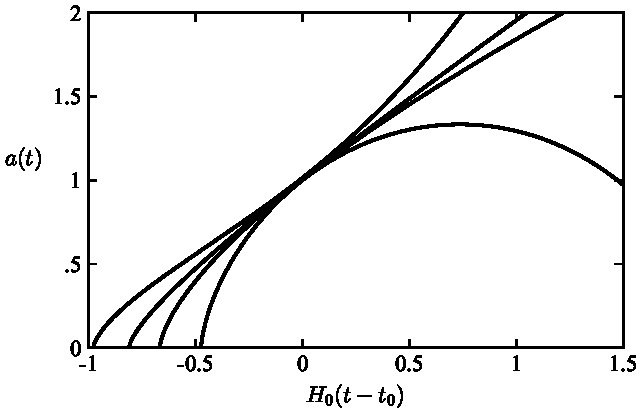
\includegraphics[width=0.72\textwidth]{fig_8.3.pdf}
\caption*{图 8.3\quad 不同 $\Omega_{\mathrm{M}}$ 与 $\Omega_{\Lambda}$ 取值下的膨胀历史。自上而下，各条曲线分别描述 $(\Omega_{\mathrm{M}},\Omega_{\Lambda})=(0.3,0.7)$、$(0.3,0.0)$、$(1.0,0.0)$ 和 $(4.0,0.0)$。}
\end{figure}

如果真空能为负，就\emph{总会}发生再度坍缩；随着宇宙膨胀，真空能最终将占据主导，而 $\Omega_{\Lambda}<0$ 的效果是导致减速和再度坍缩（正如 $\Omega_{\Lambda}>0$ 的效果是把宇宙推开）。当 $\Omega_{\Lambda}\ge0$ 时，如果 $\Omega_{\mathrm{M}}$ 大到足以在 $\Omega_{\Lambda}$ 来得及接管之前使宇宙的膨胀停下来，再度坍缩也是可能的。这些可能性表现为图 8.4 中 $\Omega_{\mathrm{M}}/\Omega_{\Lambda}$ 参数空间的不同区域。对角线代表 $\Omega_{\mathrm{total}}=1$，意味着 $\kappa=0$。

要确定永恒膨胀与最终再度坍缩之间的分界线，请注意：坍缩要求 Hubble 参量在从正变负的过程中经过零。发生这种转折处的尺度因子 $a_{*}$，可以通过在弗里德曼方程中令 $H=0$ 而求得，
\begin{equation*}
H^{2} = 0 = \frac{8\pi G}{3}\left(\rho_{\mathrm{M}0}a_{*}^{-3} + \rho_{\Lambda0} + \rho_{\mathrm{c}0}a_{*}^{-2}\right).
\tag{8.92}
\end{equation*}
把它除以 $H_0^{2}$，利用 $\Omega_{\mathrm{c}0}=1-\Omega_{\mathrm{M}0}-\Omega_{\Lambda0}$，再稍加整理，便得到
\begin{equation*}
\Omega_{\Lambda0}a_{*}^{3} + (1-\Omega_{\mathrm{M}0}-\Omega_{\Lambda})a_{*} + \Omega_{\mathrm{M}0} = 0.
\tag{8.93}
\end{equation*}
（译注：按式 (8.92) 的推导，第二项应为 $\Omega_{\Lambda0}$；原书排印漏写下标 0，原文如此。）

这是关于 $a_{*}$（转折点处的尺度因子）的三次方程。当然，我们对 $a_{*}$ 本身并不很在乎；我们在乎的是，给定 $\Omega_{\mathrm{M}0}$，使 (8.93) 存在实解的 $\Omega_{\Lambda0}$ 值。求解这个三次方程并做一些数学运算，我们发现，宇宙将永远膨胀所对应的 $\Omega_{\Lambda0}$ 值由下式给出

% ---- 书页 343 / p358 ----
\begin{figure}[H]
\centering
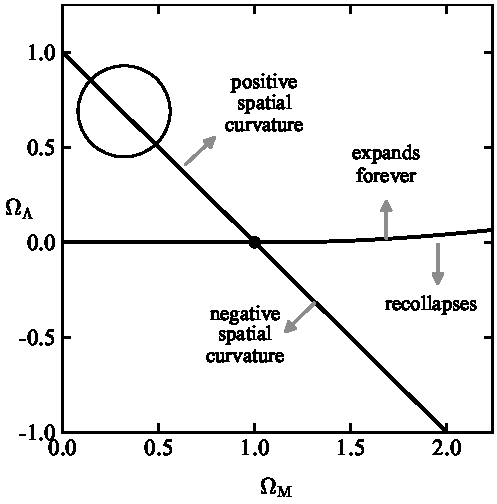
\includegraphics[width=0.72\textwidth]{fig_8.4.pdf}
\caption*{图 8.4\quad 由物质和真空能主导的宇宙的性质，表示为密度参数 $\Omega_{\mathrm{M}}$ 与 $\Omega_{\Lambda}$ 的函数。左上角的圆形区域大致代表实验数据（截至 2003 年）所偏好的数值。}
\end{figure}

\begin{equation*}
\Omega_{\Lambda0} \ge
\left\{
\begin{array}{ll}
0 & 0\le\Omega_{\mathrm{M}0}\le1 \\
4\Omega_{\mathrm{M}0}\cos^{3}\left[\dfrac{1}{3}\cos^{-1}\left(\dfrac{1-\Omega_{\mathrm{M}0}}{\Omega_{\mathrm{M}0}}\right) + \dfrac{4\pi}{3}\right] & \Omega_{\mathrm{M}0}>1.
\end{array}
\right.
\tag{8.94}
\end{equation*}
注意，当 $\Omega_{\Lambda0}=0$ 时，开放和平直宇宙（$\Omega_0=\Omega_{\mathrm{M}0}\le1$）将永远膨胀，而闭合宇宙（$\Omega_0=\Omega_{\mathrm{M}0}>1$）将再度坍缩。对宇宙学常数由来已久的轻视，造成了一种民间信念，认为这是一种必然的对应关系；然而，一旦承认真空能的可能性，空间几何与最终命运之间的任何组合就都是可能的了。

在图 8.4 的左上角，我们标出了目前受偏好的宇宙学参数取值：$\Omega_{\mathrm{M}0}\sim0.3$、$\Omega_{\Lambda0}\sim0.7$，我们将在 8.7 节中讨论。这已深入永恒膨胀的区域；如果真空能保持真正的恒定（它未必如此），我们的宇宙就注定要永远膨胀下去。

在本节的结尾，我们指出为弗里德曼方程寻找静态解的困难。要成为静态，我们必须不仅有 $\dot{a}=0$，还要 $\ddot{a}=0$。由式 (8.68)，这只有在压强为
\begin{equation*}
p = -\frac{1}{3}\rho,
\tag{8.95}
\end{equation*}
时才可能；而由式 (8.67)，还必须存在非零的空间曲率
\begin{equation*}
\frac{\kappa}{a^{2}} = \frac{8\pi G}{3}\rho.
\tag{8.96}
\end{equation*}

% ---- 书页 344 / p359 ----
由于能量密度和压强必须异号，如果我们只诉诸物质或辐射，这些条件就无法满足。当 Einstein 最初在广义相对论中寻找宇宙学解时，天文学家尚未发现宇宙正在膨胀，因此静态解的缺失曾被认为是个难题。这为 Einstein 引入宇宙学常数提供了动机；静态条件可以由物质和真空能的组合来满足，其中
\begin{equation*}
\rho_{\Lambda} = \frac{1}{2}\rho_{\mathrm{M}},
\tag{8.97}
\end{equation*}
再加上适当的正空间曲率。这些参数描述的是\textbf{Einstein 静态宇宙}（Einstein static universe）。如今我们知道宇宙在膨胀，因此这个解没有多少经验上的意义；但它对理论家却极为有用，为共形图的构造提供了基础。

\section{红移与距离}

显然，我们希望通过观测测定若干个量，以判断 FRW 模型中的哪一个对应我们的宇宙。显然我们想测定 $H_0$，因为它与宇宙的年龄有关；我们还想知道 $\Omega$，它通过式 (8.76) 决定 $\kappa$。为了理解这些量究竟可能如何被测量，让我们考虑 FRW 宇宙中的测地线运动。FRW 宇宙中存在若干类空 Killing 矢量，却没有能给我们守恒能量概念的类时 Killing 矢量。不过，确实存在一个 Killing 张量。如果 $U^{\mu}=(1,0,0,0)$ 是共动观者的四速度，那么张量
\begin{equation*}
K_{\mu\nu} = a^{2}(g_{\mu\nu} + U_{\mu}U_{\nu})
\tag{8.98}
\end{equation*}
满足 $\nabla_{(\sigma}K_{\mu\nu)}=0$（你可以自行验证），因而是一个 Killing 张量。这意味着，如果粒子具有四速度 $V^{\mu}=\mathrm{d}x^{\mu}/\mathrm{d}\lambda$，那么
\begin{equation*}
K^{2} = K_{\mu\nu}V^{\mu}V^{\nu} = a^{2}[V_{\mu}V^{\mu} + (U_{\mu}V^{\mu})^{2}]
\tag{8.99}
\end{equation*}
沿测地线将是常数。让我们先就有质量粒子的情形来思考这个问题。此时我们将有 $V_{\mu}V^{\mu}=-1$，于是
\begin{equation*}
(V^{0})^{2} = 1 + |\vec{V}|^{2},
\tag{8.100}
\end{equation*}
其中 $|\vec{V}|^{2}=g_{ij}V^{i}V^{j}$。我们还有 $U_{\mu}V^{\mu}=-V^{0}$，所以式 (8.99) 给出
\begin{equation*}
|\vec{V}| = \frac{K}{a}.
\tag{8.101}
\end{equation*}
因此，随着宇宙膨胀，粒子相对于共动坐标会“慢下来”。事实上这是一种真实的变慢，其意义是：初始相对速度很高的一团粒子气体将随宇宙膨胀而冷却下来。

% ---- 书页 345 / p360 ----
类似的事情也发生在类光测地线上。此时 $V_{\mu}V^{\mu}=0$，式 (8.99) 给出
\begin{equation*}
U_{\mu}V^{\mu} = \frac{K}{a}.
\tag{8.102}
\end{equation*}
但共动观者测得的光子频率是 $\omega=-U_{\mu}V^{\mu}$。因此，以频率 $\omega_{\mathrm{em}}$ 发出的光子，随着宇宙的膨胀将被观测到较低的频率 $\omega_{\mathrm{obs}}$：
\begin{equation*}
\frac{\omega_{\mathrm{obs}}}{\omega_{\mathrm{em}}} = \frac{a_{\mathrm{em}}}{a_{\mathrm{obs}}}.
\tag{8.103}
\end{equation*}
宇宙学家喜欢用这两个事件之间的\textbf{红移}（redshift）$z$ 来谈论它，红移由波长的分数变化定义：
\begin{equation*}
z_{\mathrm{em}} = \frac{\lambda_{\mathrm{obs}} - \lambda_{\mathrm{em}}}{\lambda_{\mathrm{em}}}.
\tag{8.104}
\end{equation*}
如果观测发生在今天（$a_{\mathrm{obs}}=a_0=1$），这意味着
\begin{equation*}
\boxed{\,a_{\mathrm{em}} = \frac{1}{1+z_{\mathrm{em}}}.\,}
\tag{8.105}
\end{equation*}
所以，一个天体的红移告诉我们光子发射时的尺度因子。

注意，这种红移与传统的多普勒效应并不是一回事；导致红移的是空间的膨胀，而不是观者与发射者的相对速度。不过，如果我们在与 Hubble 半径 $H_0^{-1}$ 以及空间曲率半径 $\kappa^{-1/2}$ 相比很小的距离上观测星系，宇宙的膨胀看上去就很像一群星系在彼此远离，红移看上去也很像多普勒效应。因此，天文学家常常用“速度”$v=cz$（$c$ 是光速）来考虑红移。尽管我们知道，对弯曲时空中不同点上的两个物体并不能真正谈论相对速度，但这个虚构的说法在足够短的距离上工作得很好。在这个近似之内，从我们到某个星系的“距离”$d$ 可以取为\textbf{瞬时物理距离}（instantaneous physical distance）$d_P$（即在诸如厘米这样的物理单位下，沿我们当前的空间超曲面量出的、我们与该星系位置之间的距离）。让我们把 RW 度规写成
\begin{equation*}
\mathrm{d}s^{2} = -\mathrm{d}t^{2} + a^{2}(t)R_0^{2}\left[\mathrm{d}\chi^{2} + S_k^{2}(\chi)\,\mathrm{d}\Omega^{2}\right],
\tag{8.106}
\end{equation*}
其中 $S_k(\chi)$ 由式 (8.33) 定义，而 $k\in\{+1,0,-1\}$。在这种形式下，在时刻 $t$ 测得的、我们（$\chi=0$）与共动径向坐标为 $\chi$ 的星系之间的瞬时物理距离就是
\begin{equation*}
d_P(t) = a(t)R_0\chi,
\tag{8.107}
\end{equation*}

% ---- 书页 346 / p361 ----
其中 $\chi$ 保持不变，因为我们假定我们和被观测的星系都完美地共动。（它们可能并不如此；在那种情形下，把所谓“本动速度”（peculiar velocities）引起的修正包括进来是轻而易举的。）当然，“距离”之所以加引号，是因为一旦离开这个近似，就有好几种彼此不等价而有用的距离概念；但当 $d_P$ 很小时它们全都一致。这时，观测到的速度（由红移推断）就简单地是
\begin{equation*}
v = \dot{d}_P = \dot{a}R_0\chi = \frac{\dot{a}}{a}d_P.
\tag{8.108}
\end{equation*}
在今天取值，它就成为
\begin{equation*}
\boxed{\,v = H_0 d_P,\,}
\tag{8.109}
\end{equation*}
这就是著名的\textbf{Hubble 定律}（Hubble law）：对于不太遥远的星系，观测到的退行速度与距离成正比。

如果红移不是非常小，我们就得更仔细地思考宇宙学中“距离”指的是什么。瞬时物理距离是一个方便的构造，但它本身不可观测，因为观测涉及的总是我们过去光锥上的事件，而不是我们当前的空间超曲面。在欧几里得空间中，推断一个物体的距离有许多不同的方法；例如，我们可以把它的视亮度与它的内禀光度相比较，或者把它的视角速度与它的内禀横向速度相比较，或者把它的视角大小与它的物理尺度相比较。对每一种情形，我们都可以定义一种距离，即假如空间是欧几里得的、宇宙不在膨胀时我们\emph{将会}推断出的距离。

让我们从\textbf{光度距离}（luminosity distance）$d_L$ 开始，它的定义是满足
\begin{equation*}
d_L^{2} = \frac{L}{4\pi F},
\tag{8.110}
\end{equation*}
其中 $L$ 是源的绝对光度，$F$ 是观者测得的流量（flux），即单位时间落到某个探测器单位面积上的能量。这个定义来自如下事实：在平直空间中，对位于距离 $d$ 处的源，流量与光度之比正好是以源为中心的球面面积的倒数，$F/L = 1/A(d) = 1/4\pi d^{2}$。然而在 FRW 宇宙中，流量将被稀释。光子数守恒告诉我们，源发出的所有光子最终都将穿过与发射者相距共动距离 $\chi$ 的球面。但流量还会被两个附加效应稀释：单个光子红移一个因子 $(1+z)$；而且光子撞击球面的频率变低，因为相隔 $\delta t$ 发出的两个光子，被观测到的相隔时间是 $(1+z)\delta t$。于是我们将有
\begin{equation*}
\frac{F}{L} = \frac{1}{(1+z)^{2}A}.
\tag{8.111}
\end{equation*}

% ---- 书页 347 / p362 ----
以共动距离 $\chi$ 为中心的球面的面积 $A$，可以从式 (8.106) 中 $\mathrm{d}\Omega^{2}$ 的系数导出，得到
\begin{equation*}
A = 4\pi R_0^{2}S_k^{2}(\chi),
\tag{8.112}
\end{equation*}
其中我们已取 $a(t)=1$，因为我们是在今天观测这些光子。把所有这些合在一起，就得到
\begin{equation*}
d_L = (1+z)R_0S_k(\chi).
\tag{8.113}
\end{equation*}
光度距离 $d_L$ 是我们有希望测量的量，因为有一些天体物理源的绝对光度是已知的。但 $\chi$ 是不可观测的，所以我们必须把它从方程中消去。在类光测地线（为方便起见取为径向）上，我们有
\begin{equation*}
0 = \mathrm{d}s^{2} = -\mathrm{d}t^{2} + a^{2}R_0^{2}\mathrm{d}\chi^{2},
\tag{8.114}
\end{equation*}
即
\begin{equation*}
\chi = R_0^{-1}\int\frac{\mathrm{d}t}{a} = R_0^{-1}\int\frac{\mathrm{d}a}{a^{2}H(a)},
\tag{8.115}
\end{equation*}
其中我们用了 $H=\dot{a}/a$。惯常的做法是用 $a=1/(1+z)$ 把尺度因子换成红移，于是我们有
\begin{equation*}
\chi(z) = R_0^{-1}\int_{0}^{z}\frac{\mathrm{d}z'}{H(z')}.
\tag{8.116}
\end{equation*}

为了计算这个积分中的 Hubble 参量，我们使用弗里德曼方程 (8.67)，像上一节中那样把它写成
\begin{equation*}
H^{2} = \frac{8\pi G}{3}\sum_{i(\mathrm{c})}\rho_i.
\tag{8.117}
\end{equation*}
为了简化问题，我们可以再次假设每个密度组分都按幂律演化，
\begin{equation*}
\rho_i(z) = \rho_{i0}a^{-n_i} = \rho_{i0}(1+z)^{n_i},
\tag{8.118}
\end{equation*}
于是我们可以写出
\begin{equation*}
H(z) = H_0E(z),
\tag{8.119}
\end{equation*}
其中
\begin{equation*}
E(z) = \left[\sum_{i(\mathrm{c})}\Omega_{i0}(1+z)^{n_i}\right]^{1/2},
\tag{8.120}
\end{equation*}

% ---- 书页 348 / p363 ----
其中密度参数 $\Omega_i$ 由式 (8.74) 定义。下面涉及 $E(z)$ 的那些方程，无论能量源是否按幂律演化都成立；若不按幂律演化，只需采用 $E(z)=H(z)/H_0$［其中 $H(z)$ 由弗里德曼方程确定］而不必用式 (8.120)。

于是，光度距离为
\begin{equation*}
d_L(z) = (1+z)R_0S_k\left[R_0^{-1}H_0^{-1}\int\frac{\mathrm{d}z'}{E(z')}\right].
\tag{8.121}
\end{equation*}
注意，当 $k=0$ 时 $R_0$ 自动消去，这很好，因为在那种情形下它是一个完全任意的参数。即使它并非任意，人们通常也更愿意用 $\Omega_{\mathrm{c}0}=-k/R_0^{2}H_0^{2}$ 来讨论；这个量既可以由对空间曲率的测定直接测量，也可以通过测量密度参数并利用 $\Omega_{\mathrm{c}0}=1-\Omega_0$ 来得到。用这个参数，我们有
\begin{equation*}
R_0 = H_0^{-1}\sqrt{-k\Omega_{\mathrm{c}0}} = \frac{H_0^{-1}}{\sqrt{|\Omega_{\mathrm{c}0}|}}.
\tag{8.122}
\end{equation*}
于是，我们把光度距离用可测量的宇宙学参数写成
\begin{equation*}
\boxed{\,d_L(z) = (1+z)\frac{H_0^{-1}}{\sqrt{|\Omega_{\mathrm{c}0}|}}S_k\left[\sqrt{|\Omega_{\mathrm{c}0}|}\int\frac{\mathrm{d}z'}{E(z')}\right].\,}
\tag{8.123}
\end{equation*}
这个方程虽然显得笨拙，却在宇宙学中处于核心地位。给定可观测量 $H_0$ 和 $\Omega_{i0}$，我们可以直接算出到位于任一红移 $z$ 处天体的光度距离；同样地，我们也可以对一系列红移范围内的天体测量 $d_L(z)$，并从这些信息中提取 $H_0$ 和/或各个 $\Omega_{i0}$。

除光度距离之外，还有两个相关的距离量度。正如光度距离是假如我们身处平直空间时，从源的内禀光度和观测光度推断出的距离，\textbf{固有运动距离}（proper motion distance）$d_M$ 是从源的内禀运动和观测运动推断出的距离。它的定义为
\begin{equation*}
d_M = \frac{u}{\dot{\theta}},
\tag{8.124}
\end{equation*}
其中 $u$ 是固有横向速度（比如你会以 k/s 为单位来测量的量），而 $\dot{\theta}$ 是观测到的角速度。另一方面，\textbf{角直径距离}（angular diameter distance）是从源的内禀大小和观测大小推断出的距离；它的定义为
\begin{equation*}
d_A = \frac{R}{\theta},
\tag{8.125}
\end{equation*}

% ==== tail：8.5 节（红移与距离）收尾，承接书页 348 末的 (8.125)，
% ==== 至书页 349 中 8.6 节标题之前；置于本文件第一个 \section 之前 ====

% ---- 书页 349 / p364 ----
%JOIN%其中 $R$ 是天体的固有大小，$\theta$ 是观测到的角直径。在这两种情形下，我们都能导出与式 (8.123) 类似的公式；所幸，对宇宙学参数的那种难以驾驭的依赖关系为所有距离量度所共有，最后剩下的只是对红移的简单依赖：
\begin{equation*}
d_L = (1+z)d_M = (1+z)^{2}d_A,
\tag{8.126}
\end{equation*}
鼓励各位动手验证一下。这样，只要测得了其中一种距离，我们就能方便地换算成其他任何一种；或者，我们也可以独立地测量不同的距离，并利用式 (8.126) 来检验 RW 框架的自洽性。

趁我们还在思量距离，不妨也考虑一下：从红移为 $z$ 的天体发出的光，从发射时刻到现在流逝了多长时间。如果宇宙今天的年龄是 $t_0$，而光子被发射时宇宙的年龄是 $t_{*}$，那么\textbf{回溯时间}（lookback time）为
\begin{align*}
t_0 - t_{*} &= \int_{t_{*}}^{t_0}\mathrm{d}t\\
&= \int_{a_{*}}^{1}\frac{\mathrm{d}a}{aH(a)}\\
&= H_0^{-1}\int_0^{z_{*}}\frac{\mathrm{d}z'}{(1+z')E(z')}.
\tag{8.127}
\end{align*}
例如，考虑一个平直（$k=0$）、物质主导（$\rho=\rho_{\mathrm{M}}=\rho_{\mathrm{M}0}a^{-3}$）的宇宙。那么
\begin{equation*}
E(z) = (1+z)^{3/2},
\tag{8.128}
\end{equation*}
于是
\begin{align*}
t_0 - t_{*} &= H_0^{-1}\int_0^{z_{*}}\frac{\mathrm{d}z'}{(1+z')^{5/2}}\\
&= \frac{2}{3}H_0^{-1}\left[1-(1+z_{*})^{-3/2}\right].
\tag{8.129}
\end{align*}
令 $t_{*}\to 0$（$z_{*}\to\infty$），便得到物质主导宇宙的总年龄：
\begin{equation*}
t_0(\mathrm{MD}) = \frac{2}{3}H_0^{-1}.
\tag{8.130}
\end{equation*}
对于并非完全物质主导的宇宙，$\frac{2}{3}$ 这个因子不会完全正确，但对于合理的宇宙学参数取值，我们通常得到 $t_0\sim H_0^{-1}$。

\section{引力透镜}

在第 7 章中我们介绍了引力透镜（gravitational lensing）的概念：光在 Newton 引力场中的偏折与时间延迟。除了在太阳系内为广义相对论提供检验之外，透镜效应还出现在众多天体物理情境之中，并已成为现代宇宙学不可或缺的组成部分。\footnote{关于引力透镜的一篇优秀综述——我们的讨论即从中借鉴——参见 R.~Narayan and M.~Bartelmann, ``Lectures on Gravitational Lensing,'' 13th Jerusalem Winter School in Theoretical Physics, \texttt{http://arxiv.org/astro-ph/9606001}。}

% ---- 书页 350 / p365 ----
\begin{figure}[H]
\centering
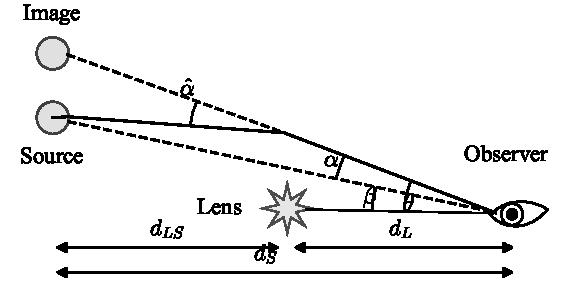
\includegraphics[width=0.72\textwidth]{fig_8.5.pdf}
\caption*{图 8.5\quad 引力透镜的几何，概括于透镜方程 (8.132) 之中。透镜的作用，是把平直 Minkowski 背景中本应观测到的角 $\beta$ 扭变为角 $\theta$。}
\end{figure}

宇宙学透镜效应与我们先前讨论的情形有两个重要区别：Robertson--Walker 度规取代了 Minkowski 背景，而且透镜本身往往也比简单的点质量复杂。图 8.5 描绘了一种典型的透镜几何。在这一节的讨论中，我们将始终假设透镜是“薄”的——即其空间延展尺度远小于源、透镜与观者之间的距离。在这种情形下，我们可以合理地谈论一个唯一的到透镜的距离 $d_L$，以及透镜到源的距离 $d_{LS}$。

对于天空上一幅（可能很复杂的）像，我们用像的不同成分之间的一组夹角来描述它。这些夹角可以看作天空上的二维矢量。透镜的作用，是把没有任何偏折时本应观测到的那些角——例如源与透镜之间的夹角 $\vec{\beta}$——扭变为一幅由一组角 $\vec{\theta}$ 刻画的新像。我们全程假设这些角都很小。这一映射由\textbf{约化透镜角}（reduced lensing angle）$\vec{\alpha}=\vec{\theta}-\vec{\beta}$ 描述。按照图 8.5 所示的几何，它与真实偏转角 $\widehat{\vec{\alpha}}$ 之间的关系为
\begin{equation*}
\vec{\alpha} = \frac{d_{LS}}{d_S}\widehat{\vec{\alpha}}.
\tag{8.131}
\end{equation*}

% ---- 书页 351 / p366 ----
于是我们得到\textbf{透镜方程}（lens equation）
\begin{equation*}
\boxed{\,\vec{\beta} = \vec{\theta} - \frac{d_{LS}}{d_S}\widehat{\vec{\alpha}}.\,}
\tag{8.132}
\end{equation*}
透镜方程所描述的，无非是受扰时空中的光线追踪。

当然，我们应当仔细琢磨图中画出的那些“距离” $d_i$。透镜效应发生在膨胀的宇宙中，而宇宙还可能带有空间曲率。不过，只要我们\emph{定义}距离 $d_i$ 使得透镜方程所描述的几何关系得以成立，透镜方程就依然成立。换言之，这些距离是：在静态欧几里得空间背景中，给定夹角与横向物理尺度时我们本会推断出的距离。而这恰恰就是角直径距离 (8.125) 的定义。因此，本节中的所有距离都取为角直径距离。注意，角直径距离未必能够相加，故 $d_S\neq d_L+d_{LS}$。

举一个简单的例子：点质量透镜。在第 7 章研究 Newton 极限时我们曾经发现，光子穿过引力势 $\Phi$ 时的偏转角由下式给出：
\begin{equation*}
\widehat{\vec{\alpha}} = 2\int \vec{\nabla}_{\perp}\Phi\,\mathrm{d}s,
\tag{8.133}
\end{equation*}
对于碰撞参数为 $b$ 的点质量 $M$，上式化为
\begin{equation*}
\widehat{\vec{\alpha}} = \frac{4GM}{b}.
\tag{8.134}
\end{equation*}
碰撞参数可以写成 $b=d_L\theta$。透镜方程 (8.132) 便成为
\begin{equation*}
\beta = \theta - \frac{d_{LS}}{d_S d_L}\frac{4GM}{\theta}.
\tag{8.135}
\end{equation*}
富有启发性的做法是考虑最简单的情形：源与透镜共线（$\beta=0$）。此时源将被透镜成一个环绕透镜的\textbf{Einstein 环}（Einstein ring），其角距离由\textbf{Einstein 角}（Einstein angle）给出：
\begin{equation*}
\theta_{\mathrm{E}} = \sqrt{\frac{4GMd_{LS}}{d_L d_S}}.
\tag{8.136}
\end{equation*}
即便在更复杂的位形中，Einstein 角也为透镜效应设定了一个特征尺度。我们还可以定义一个与之相联系的距离尺度，即\textbf{Einstein 半径}（Einstein radius）：
\begin{equation*}
R_{\mathrm{E}} = \sqrt{\frac{4GMd_L d_{LS}}{d_S}}.
\tag{8.137}
\end{equation*}

% ---- 书页 352 / p367 ----
换算成厘米或其他物理单位时，别忘了在我们的所有方程中都有 $c=1$。为了对典型天体物理情形下透镜效应的大小有些感觉，我们可以考虑两种常见的场合：我们银河系内近似太阳质量的天体造成的“微透镜”（microlensing），以及星系或星系团造成的宇宙学透镜。前一情形下 Einstein 角将是毫角秒的量级，而后一情形下则是角秒的量级：
\begin{align*}
\theta_{\mathrm{E}} &= 0.9\sqrt{\left(\frac{M}{M_{\odot}}\right)\left(\frac{10\ \mathrm{kpc}}{D}\right)}\ \text{毫角秒}\\
&= 0.9\sqrt{\left(\frac{M}{10^{11}M_{\odot}}\right)\left(\frac{\mathrm{Gpc}}{D}\right)}\ \text{角秒}.
\tag{8.138}
\end{align*}
我们暂时继续讨论点质量透镜。尽管已经观测到若干例壮观的 Einstein 环，但多数时候我们不会幸运到源与透镜恰好完美对齐。这时我们可以求解 (8.135)，得到像角的两个数值：
\begin{equation*}
\theta_{\pm} = \frac{1}{2}\left(\beta \pm \sqrt{\beta^{2}+4\theta_{\mathrm{E}}^{2}}\right).
\tag{8.139}
\end{equation*}
位于 $\theta_{+}$ 处的像总在 Einstein 角之外，而 $\theta_{-}$ 处的像则在其内。实际上这个公式有些误导性：像的数目永远会是奇数；对点质量透镜而言，第三个像将位于与透镜自身相同的位置。

现在来考虑比点质量更一般的透镜。我们知道，偏转角可以借助 Newton 引力势由式 (8.133) 给出。我们可以沿从观者出发指向过去的测地线路径作积分，定义\textbf{透镜势}（lensing potential）：
\begin{equation*}
\psi(\vec{\theta}) = 2\frac{d_{LS}}{d_L d_S}\int \Phi(d_L\vec{\theta},s)\,\mathrm{d}s.
\tag{8.140}
\end{equation*}
利用透镜势，只需取梯度便可直接导出约化透镜角：
\begin{align*}
\vec{\alpha} &= \vec{\nabla}_{\theta}\psi\\
&= 2\frac{d_{LS}}{d_S}\int \vec{\nabla}_{\perp}\Phi\,\mathrm{d}s.
\tag{8.141}
\end{align*}
注意，角梯度 $\vec{\nabla}_{\theta}$ 与 $\vec{\nabla}_{\perp}$（对透镜所在处横向距离的梯度）相差一个因子 $d_L$。薄透镜近似使我们可以把积分收缩为在透镜位置上取值的量。我们还可以对透镜势作用（二维）拉普拉斯算符，得到\textbf{会聚}（convergence）$\kappa$：
\begin{align*}
\kappa(\vec{\theta}) &\equiv \frac{1}{2}\nabla_{\theta}^{2}\psi\\
&= \frac{d_L d_{LS}}{d_S}\int \nabla^{2}\Phi\,\mathrm{d}s.
\tag{8.142}
\end{align*}

% ---- 书页 353 / p368 ----
会聚可以被看作对积分质量密度的一种量度。我们可以把上面的表达式反过来，用会聚同时写出透镜势与约化偏转角：
\begin{equation*}
\psi(\vec{\theta}) = \frac{1}{\pi}\int \kappa(\vec{\theta}\,')\ln|\vec{\theta}-\vec{\theta}\,'|\,\mathrm{d}^{2}\theta'
\tag{8.143}
\end{equation*}
以及
\begin{equation*}
\vec{\alpha}(\vec{\theta}) = \frac{1}{\pi}\int \kappa(\vec{\theta}\,')\frac{\vec{\theta}-\vec{\theta}\,'}{|\vec{\theta}-\vec{\theta}\,'|}\,\mathrm{d}^{2}\theta'.
\tag{8.144}
\end{equation*}
要检验这些方程，请记住这些矢量只定义在两个横向维度上。

会聚描述的是引力透镜对光线的聚焦。这种聚焦使源显得更大（就像放大镜一样）。根据 Liouville 定理——源所发射光子的相空间密度守恒——源的面亮度在透镜作用下保持不变；因此尺度的增大导致亮度的放大。与此同时，光线穿过透镜时的扭转还会引起畸变，导致像的形状发生切变。为了描述这两种现象，我们考虑透镜映射的导数所构成的 $2\times 2$ 矩阵
\begin{equation*}
A_{ij} \equiv \frac{\partial\beta^{i}}{\partial\theta^{j}}.
\tag{8.145}
\end{equation*}
注意，上、下指标之间实际上没有区别，因为它们定义在二维欧几里得平面上。由于 $\vec{\beta}=\vec{\theta}-\vec{\alpha}$，我们有
\begin{align*}
A_{ij} &= \delta_{ij} - \frac{\partial\alpha^{i}}{\partial\theta^{j}}\\
&= \delta_{ij} - \psi_{ij},
\tag{8.146}
\end{align*}
这里我们引入了记号
\begin{equation*}
\psi_{ij} \equiv \frac{\partial^{2}\psi}{\partial\theta^{i}\partial\theta^{j}}.
\tag{8.147}
\end{equation*}
矩阵 $A$ 编码了透镜映射的局域性质。它的逆矩阵被称为\emph{放大张量}（magnification tensor）
\begin{equation*}
\boldsymbol{M} = \frac{\partial\vec{\theta}}{\partial\vec{\beta}} = A^{-1}.
\tag{8.148}
\end{equation*}

% ---- 书页 354 / p369 ----
这个名字从何而来？透镜把由 $\vec{\beta}$ 描述的面元扭变为由 $\vec{\theta}$ 描述的面元，面积的改变由这个映射的雅可比行列式描述，而后者无非是 $\boldsymbol{M}$ 的行列式。这个行列式被定义为\textbf{放大率}（magnification）$\mu$：
\begin{equation*}
\mu = |\boldsymbol{M}| = \frac{1}{|A|}.
\tag{8.149}
\end{equation*}
$\mu$ 的绝对值告诉我们源的亮度实际改变了多少；$\mu$ 可能为负，这意味着像的奇偶性被翻转了。我们说“放大”，是因为只有当透镜和源在天空中彼此靠近时透镜效应才会惹人注意，此时聚焦效应只会带来视亮度的增加；而一个远离源（在天空中位置相距甚远）的透镜所导致的光度极微小的减少，则永远不会被注意到。（如果存在多重像，所有像的亮度之和将超过未畸变源的亮度。）

$A$ 的分量可以分解为会聚与切变的效应。对于会聚，由 $\kappa=\frac{1}{2}\nabla_{\theta}^{2}\psi$ 可得
\begin{equation*}
\kappa = \frac{1}{2}(\psi_{11}+\psi_{22}).
\tag{8.150}
\end{equation*}
而\textbf{切变}（shear）则使源的形状发生畸变；如果初始为圆形的源被畸变为椭圆度为 $\gamma$、方位角为 $\phi$ 的椭圆，我们定义切变的两个分量为
\begin{align*}
\gamma_1 &= \gamma\cos(2\phi)\\
\gamma_2 &= \gamma\sin(2\phi),
\tag{8.151}
\end{align*}
于是总切变为 $\gamma=\sqrt{\gamma_1^{2}+\gamma_2^{2}}$。用透镜势表出，这些分量为
\begin{align*}
\gamma_1 &= \frac{1}{2}(\psi_{11}-\psi_{22})\\
\gamma_2 &= \psi_{12}=\psi_{21}.
\tag{8.152}
\end{align*}
反解这些关系以求出 $A$ 的分量，得到
\begin{equation*}
A = \begin{pmatrix} 1-\kappa-\gamma_1 & -\gamma_2\\ -\gamma_2 & 1-\kappa+\gamma_1 \end{pmatrix}.
\tag{8.153}
\end{equation*}
于是我们可以用会聚与切变来表示放大率：
\begin{equation*}
\mu = \frac{1}{(1-\kappa)^{2}-\gamma^{2}}.
\tag{8.154}
\end{equation*}

% ---- 书页 355 / p370 ----
透镜效应的这些特征在观测宇宙学中正变得日益重要。显然令人感兴趣的是所谓“强透镜”（strong lensing）的情形：源位于透镜的 Einstein 半径之内，这时可能形成多重像。通过观测同一源的多个像，我们可以推断透镜质量分布的性质（例如用来搜寻暗物质）；我们还可以利用不同路径上的时间延迟来测量 Hubble 常数，并利用透镜事件的统计频率来约束其他宇宙学参数。不过，透镜效应不必很强也能产生重要影响。“弱透镜”（weak lensing）——源与透镜相距超过一个 Einstein 半径——一般导致少量的放大与切变，若不预先知道源的性质便无法探测。然而，切变效应可以用统计方法探测：考察成千上万个星系的形状（假定它们的取向本质上是随机的）。弱透镜切变导致这些形状出现相关联的畸变，从而可以揭示观者与遥远源之间物质分布的大量信息。

\section{我们的宇宙}

在讨论 FRW 宇宙学的行为时，我们屡次提及与我们身处的宇宙相对应的宇宙学参数的实际取值。现在让我们更系统一些：既讨论我们今天看到的宇宙，也讨论向早期时刻的合理外推。我们的讨论必然简略，这既出于篇幅考虑，也因为宇宙学是一个活跃的研究领域；想要了解当前观点的最新描述，请查阅近期的综述文章。

我们对膨胀率的许多直接测定，依靠的是把光度距离公式 (8.123) 应用于某种其内禀光度被假定已知的天体，这类天体称为\textbf{标准烛光}（standard candles）。（偶尔我们也测量其内禀尺度被假定已知的物体的角直径：标准尺［standard rulers］。）例如，Hubble 常数就是用各种标准烛光测量的，不同方法达成的共识收敛于前面提到的值 $H_0=70\pm 10$ km/sec/Mpc。高红移处对线性 Hubble 定律 (8.109) 的偏离可以提供关于密度参数 $\Omega_{i0}$ 的信息，但前提是我们必须拥有非常明亮、且内禀光度已被精确掌握的天体。Ia 型超新星（Type Ia supernovae）恰好提供了这样的天体；它们被认为是白矮星吸积了足够多的质量、以至于超过 Chandrasekhar 极限之后发生的爆发。由于 Chandrasekhar 极限接近普适，相应的爆发在本质上亮度相同（而且一部分内禀变化实际上可以通过追踪亮度随时间的演化而加以扣除）。正是在红移 $z>0.3$ 处对 Ia 型超新星的测量，提供了宇宙学常数非零的第一个直接证据；这些观测意味着 $\Omega_{\Lambda}$ 实际上大于 $\Omega_{\mathrm{M}}$。回想一下：物质是无压强的，$p_{\mathrm{M}}=0$，而真空能则伴随着负压强，$p_{\Lambda}=-\rho_{\Lambda}$。代入第二个弗里德曼方程 (8.68)，我们发现一个同时含有物质与 $\Lambda$ 的宇宙服从

% ---- 书页 356 / p371 ----
\begin{equation*}
\frac{\ddot{a}}{a} = -\frac{4\pi G}{3}(\rho_{\mathrm{M}} - 2\rho_{\Lambda}).
\tag{8.155}
\end{equation*}
于是，如果 $\rho_{\Lambda}$ 相对于 $\rho_{\mathrm{M}}$ 足够大（正如超新星观测所表明的），我们就可以有 $\ddot{a}>0$：一个加速膨胀的宇宙（其含义如 8.4 节所述）。

物质密度本身的测量方法多种多样，通常包括通过寻找成团物质的引力效应来测量密度 $\rho_{\mathrm{M}}$，然后再外推到大尺度。由于 $\rho_{\mathrm{M}}=(3H^{2}/8\pi G)\Omega_{\mathrm{M}}$，用这种方式得到的限值常常以 $\Omega_{\mathrm{M}}h^{2}$ 的形式给出，其中 $h$ 定义于式 (8.70)。如今 $H_0$ 的不确定度看来已足够小，取 $h^{2}\approx 0.5$ 相当稳妥，从此以后我们就这么做。当代的大多数方法都与如下结果一致：
\begin{equation*}
\Omega_{\mathrm{M}0} = 0.3\pm 0.1.
\tag{8.156}
\end{equation*}
在宇宙学常数获得充分的观测证据之前，如此低的物质密度有时曾被当作空间负弯曲（$\kappa<0$）的迹象。

除物质与宇宙学常数之外，宇宙中还有辐射。普通光子是辐射密度中最显然的成分，但任何相对论性粒子都会作出贡献。就光子而言，绝大部分能量密度蕴藏于宇宙微波背景——大爆炸遗留下来的辐射——之中。除光子外，辐射成分唯一显然的候选者是中微子。我们预期遗迹背景中微子的数密度与光子相当；光子的数密度可能还要稍大一些，因为在中微子数目固定下来之后，光子仍能继续产生。然而，如果中微子的质量足够大（大于约 $10^{-4}$ eV），它们今天将已经成为非相对论性的，从而对物质而非辐射作出贡献。目前关于中微子质量的看法提示情况很可能如此，但也并非完全清楚。此外，可以设想在我们已知的粒子之外，还存在迄今尚未探测到的无质量粒子（尽管它们不能太多，否则会抑制大尺度结构的形成）。总而言之，总辐射密度看来很可能与光子密度处于同一数量级；在这种情形下我们将有
\begin{equation*}
\Omega_{\mathrm{R}0} \sim 10^{-4}.
\tag{8.157}
\end{equation*}
如前所述，辐射密度低于物质密度并不令人惊讶，因为随着宇宙的膨胀，前者衰减得更快。辐射密度按 $a^{-4}$ 变化，而物质中的密度按 $a^{-3}$ 变化；因此物质-辐射相等发生的红移为
\begin{equation*}
z_{\mathrm{eq}} \approx \frac{\Omega_{\mathrm{M}0}}{\Omega_{\mathrm{R}0}} \sim 3\times 10^{3}.
\tag{8.158}
\end{equation*}

% ---- 书页 357 / p372 ----
对宇宙学参数的另一个关键约束来自微波背景温度的各向异性。平均温度为 $T_{\mathrm{CMB}}=2.74\,\mathrm{K}$，但 1992 年 COBE 卫星发现了随地点起伏、幅度为 $\Delta T/T\sim 10^{-5}$ 的涨落。这些各向异性有多种来源，其中包括复合时光子移出势阱带来的引力红移/蓝移（Sachs--Wolfe 效应，在大角尺度上占主导）、最后散射面上的内禀温度涨落（在小角尺度上占主导），以及等离子体运动的多普勒效应。描写 CMB 各向异性演化的物理超出了本书的范围。整幅天空的 CMB 温度图显然包含大量信息，但没有任何理论预言任意给定点处的温度应该是多少；现代理论预言的，一般是任意给定角尺度上各向异性大小的期望值。因此，我们把各向异性场按球谐函数展开：
\begin{equation*}
\frac{\Delta T}{T}(\theta,\phi) = \sum_{lm} a_{lm}Y_{lm}(\theta,\phi).
\tag{8.159}
\end{equation*}
$|a_{lm}|^{2}$ 的期望值很可能与 $m$ 无关；否则各向异性的统计特性会随天空中的位置而改变（尽管我们对此应当保持开放的心态）。因此，有待测量的相关参数是
\begin{equation*}
C_l = \langle|a_{lm}|^{2}\rangle.
\tag{8.160}
\end{equation*}
由于对任意固定的 $l$，$m$ 有 $2l+1$ 个可能的取值（从 $-l$ 到 $l$），除了最低的几个 $l$ 之外，对 $a_{lm}$ 的独立测量足以精确确定它们的期望值。在非常小的 $l$ 处这种不可约的不确定度被称为宇宙方差（cosmic variance）。

已有大量实验测量了 $C_l$（所谓的 CMB 功率谱），而改进这些测量在今后若干年内很可能仍是一项重要任务。（除温度各向异性之外，CMB 的偏振也包含大量信息，是另一个需要相当多实验努力的目标。）要把这些观测转化为有用的信息，我们需要一个具体的理论来预言 CMB 功率谱如何作为宇宙学参数的函数而变化。有两种领先的可能性（尽管其中一种比另一种要领先得多）：要么密度扰动在极早的时刻就被印记在所有尺度上——甚至包括物理波长 $\lambda$ 远大于 Hubble 半径 $H^{-1}$ 的模式；要么局部的动力学机制在所有时期充当各向异性的源。后一种可能性已基本上被 CMB 数据排除：如果各向异性是连续产生的，我们预期会看到相当平滑、无特征的 $C_l$ 谱，而观测却显示出显著的结构。因此，更流行的做法是设想某种原初的扰动源，例如暴胀（下一节讨论）。暴胀扰动是绝热的——物质密度中的扰动与辐射密度中的扰动相关联——并且在所有尺度上幅度几乎相等。有了这个输入，我们就可以对 $C_l$ 作出作为所有宇宙学参数函数的明确预言。迄今从实验得到的最重要约束或许是：宇宙在空间上是平直的，或至少非常接近平直；$|\Omega_{\mathrm{c}0}|<0.1$。结合物质密度的测量 $\Omega_{\mathrm{M}}\approx 0.3$，我们得出结论：真空能密度参数应为

% ---- 书页 358 / p373 ----
\begin{equation*}
\Omega_{\Lambda 0} = 0.7\pm 0.1.
\tag{8.161}
\end{equation*}
这与上面描述的 Ia 型超新星结果符合得很好；这里描述的调和图像（concordance picture）正是图 8.4 所指示的那一种。利用 $H_0=70$ km/sec/Mpc 把密度参数换算成物理能量密度，得到
\begin{equation*}
\rho_{\mathrm{vac}} \approx 10^{-8}\ \mathrm{erg/cm^{3}},
\tag{8.162}
\end{equation*}
如 4.5 节讨论真空能时所述。

我们的现今宇宙概貌还有一个值得注意的特征。前面提到，我们宇宙中约 $30\%$ 的能量密度由物质组成。但对宇宙学家而言，“物质”是任何非相对论性粒子的集合；我们通过其引力影响推断出的物质，未必是我们在地球上的经验所熟悉的那种普通物质。\textbf{普通物质}（ordinary matter）指由原子及其成分（质子、中子和电子）构成的一切东西；这包括宇宙中所有的恒星、行星、气体和尘埃，无论能否直接看到。这类物质偶尔也被称为\emph{重子物质}（baryonic matter），其中重子包括质子、中子以及相关的粒子（携带一个被称为重子数的守恒量子数的强相互作用粒子）。当然，电子在概念上是普通物质的重要部分，但按质量计算，与质子和中子相比可以忽略：
\begin{gather*}
m_p = 0.938\ \mathrm{GeV}\\
m_n = 0.940\ \mathrm{GeV}\\
m_e = 0.511\times 10^{-3}\ \mathrm{GeV}.
\tag{8.163}
\end{gather*}
换句话说，普通物质的质量绝大部分来自重子。

事实证明，普通的重子物质远不足以解释观测到的密度 $\Omega_{\mathrm{M}}\approx 0.3$。我们目前对重子密度的最佳估计给出
\begin{equation*}
\Omega_{\mathrm{b}} = 0.04\pm 0.02,
\tag{8.164}
\end{equation*}
这些误差限按大多数标准衡量都是保守的。这一测定来自多种方法：直接计数重子（最不精确的方法）、与 CMB 功率谱（上文讨论过）的一致性，以及与大爆炸核合成（下文讨论）对轻元素丰度的预言相符。因此，物质密度的大部分必定采取\textbf{非重子暗物质}（nonbaryonic dark matter）的形式，我们将把它简称为“暗物质”。（重子也可以是暗的，但越来越普遍的用法是把这一术语保留给非重子成分。）粒子物理标准模型中的每一种已知粒子，作为这种暗物质的候选者都已被排除。幸运的是，标准模型之外还有若干看似合理的候选者，包括中性伴随子（neutralino，超对称性所预言的附加稳定粒子中最轻者，质量 $\geq 100$ GeV）和轴子（axion，因假设的 Peccei--Quinn 对称性自发破缺而产生的轻赝标量粒子，引入该对称性是为了解释强相互作用中 CP 的守恒，质量 $\sim 10^{-4}$ eV）。关于暗物质，我们仅有的几点确切认识之一是：它必须是冷的——不仅今天是非相对论性的，而且在很长一段时间里都必须如此。如果暗物质是热的，它就会自由流出高密度区，抑制星系的形成。关于冷暗物质（cold dark matter，CDM）我们知道的另一件事是，它与普通物质的相互作用必须非常微弱，这样才能解释它为何迄今未被探测到。尽管如此，环境中的暗物质粒子偶尔仍可能与地球实验室里经过仔细屏蔽的探测器发生散射；通过搜寻这种散射的效应来直接探测暗物质，将是今后若干年里另一项重要的实验努力。

% ---- 书页 359 / p374 ----
$\Omega_{\mathrm{M}}=0.3$、$\Omega_{\Lambda}=0.7$ 的这幅图像，似乎能拟合种类多得令人印象深刻的观测数据。这幅图中最令人惊讶的部分是宇宙学常数。在第 4 章中我们提到，对真空能的朴素估计给出的结果比测量值大许多个数量级。实际上有三个相互关联的谜题：为什么宇宙学常数比我们预期的小这么多？构成当前宇宙 $70\%$ 的那份小小的非零能量，其起源是什么？还有，为什么真空能的当前值与物质密度处于同一数量级？最后一个问题尤其严峻，因为真空能与物质密度彼此之间演化得很快：
\begin{equation*}
\frac{\Omega_{\Lambda}}{\Omega_{\mathrm{M}}} \propto a^{3}.
\tag{8.165}
\end{equation*}
如果 $\Omega_{\mathrm{M}}$ 和 $\Omega_{\Lambda}$ 今天彼此相当，那么过去真空能会小得探测不到，而将来物质密度将变得可以忽略。这个“巧合问题”（coincidence problem）迄今仍完全是个谜。有人提出的解法涉及“人择原理”（anthropic principle）：如果宇宙存在许多不同的部分（在空间上，甚至在波函数的不同分支上），其中宇宙学常数取非常不同的数值，那么智慧生命最有可能出现在那些绝对值不太大的地方——一个大的正 $\Lambda$ 会在星系形成之前把粒子撕开，而一个大的负 $\Lambda$ 会使宇宙在生命演化出来之前就再度坍缩。对观测到的真空能的人择解释与数据拟合得很好，尽管为解释这一个量就需要求助如此精巧的方案，在一些人看来有点夸张。

另一种可能与巧合问题有关（也可能无关）的想法是：我们探测到的并非非零的宇宙学常数，而是一个紧密切拟真空能性质的动力学成分。对这种可能性的考虑，促使宇宙学家创造了\textbf{暗能量}（dark energy）这个术语，用来称呼无论实际上是什么的被探测到的东西——不管它是动力学的，还是最终被证明就是宇宙学常数。关于暗能量我们知道的是：它在空间中的分布相对平滑（否则它就会像暗物质那样，通过其局部引力场被探测到），并且随时间演化得很慢（否则它就不会像超新星数据所表明的那样使宇宙加速）。暗能量的一个简单的动力学候选者由缓慢滚动的标量场提供。考虑一个具有通常作用量的场 $\phi$：

% ---- 书页 360 / p375 ----
\begin{equation*}
S = \int \mathrm{d}^{4}x\sqrt{-g}\left[-\frac{1}{2}g^{\mu\nu}\nabla_{\mu}\phi\nabla_{\nu}\phi - V(\phi)\right],
\tag{8.166}
\end{equation*}
其能量-动量张量为
\begin{equation*}
T_{\mu\nu} = \nabla_{\mu}\phi\nabla_{\nu}\phi + \left[\frac{1}{2}g^{\rho\sigma}\nabla_{\rho}\phi\nabla_{\sigma}\phi - V(\phi)\right]g_{\mu\nu}
\tag{8.167}
\end{equation*}
而运动方程为
\begin{equation*}
\Box\phi - \frac{\mathrm{d}V}{\mathrm{d}\phi} = 0.
\tag{8.168}
\end{equation*}
假设场在空间中完全均匀（$\partial_i\phi=0$）。于是利用 Christoffel 符号 (8.44)，我们可以用时间导数和 Hubble 常数表示 d'Alembert 算符，把 (8.168) 写成
\begin{equation*}
\ddot{\phi} + 3H\dot{\phi} + \frac{\mathrm{d}V}{\mathrm{d}\phi} = 0.
\tag{8.169}
\end{equation*}
我们看到，Hubble 参量起到摩擦项的作用；场会趋于沿势滚落，但当 $H$ 太大时运动将被阻尼。因此，具有足够平坦的势的标量场（如图 8.6 所绘）将滚动得非常缓慢，导致动能远小于势能 $V(\phi)$。此时能量-动量张量为
\begin{equation*}
T_{\mu\nu} \approx -V(\phi)g_{\mu\nu},
\tag{8.170}
\end{equation*}
\begin{figure}[H]
\centering
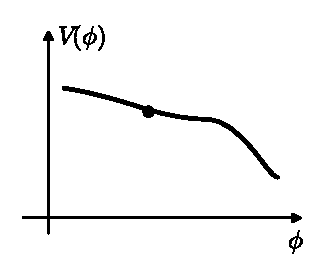
\includegraphics[width=0.72\textwidth]{fig_8.6.pdf}
\caption*{图 8.6\quad 缓慢滚动的标量场的势能。}
\end{figure}
其中 $\phi\approx$ 常数。与式 (4.96) 比较，我们看到标量场势正在摹拟一种真空能。举一个简单的例子，考虑二次势 $V(\phi)=\frac{1}{2}m^{2}\phi^{2}$。这时 (8.169) 描写一个阻尼谐振子，若 $H>m$ 就会出现过阻尼。但在粒子物理单位制中，今天的 Hubble 常数为 $H_0\approx 10^{-33}$ eV，所以这个标量场的质量将不得不比式 (8.163) 中我们熟悉的基本粒子的质量小得难以置信。这看起来像是不自然的微调。尽管如此，动力学暗能量模型正在被积极探索，部分是出于这样的希望：它们能以某种方式通向巧合问题的解决。

% ---- 书页 361 / p376 ----
有了对当代状况的这一认识，我们就可以设想，早期宇宙必须是什么样子，才能产生出我们今天看到的一切。为了物理直观，标记所考虑的时代时，用温度来表示往往比用红移或大爆炸以来的时间更有帮助。今天的温度是
\begin{equation*}
T_0 = 2.74\ \mathrm{K} = 2.4\times 10^{-4}\ \mathrm{eV}.
\tag{8.171}
\end{equation*}
当然，这里说“温度”，我们指的是宇宙微波背景的表观黑体温度；实际上 CMB 自复合以来就不再处于热平衡，所以对这个概念不宜过分当真。在绝热膨胀下，随着每种相对论性粒子红移，温度都在下降，我们有 $T\propto a^{-1}$。但在早期宇宙的特定时刻会发生非绝热相变；在这种情形下温度实际上并不会升高，只是下降得更加缓慢。为了帮助建立温度、密度与尺度因子之间的关系，我们引入\textbf{相对论性自由度的有效数目}（effective number of relativistic degrees of freedom）的两种不同量度：$g_{*}$ 与 $g_{*S}$（其中 $S$ 代表熵）。考虑一组玻色子与费米子物种，每一种都有自己的有效温度 $T_i$ 和自旋态数目 $g_i$。例如，无质量光子有两个自旋态，故 $g_{\gamma}=2$；有质量的 $\frac{1}{2}$ 自旋费米子也有两个自旋态，故 $g_{e^-}=g_{e^+}=2$。相对论性自由度有效数目的这两个不同版本满足
\begin{equation*}
g_{*} = \sum_{\mathrm{bosons}} g_i\left(\frac{T_i}{T}\right)^{4} + \frac{7}{8}\sum_{\mathrm{fermions}} g_i\left(\frac{T_i}{T}\right)^{4}
\tag{8.172}
\end{equation*}
而
\begin{equation*}
g_{*S} = \sum_{\mathrm{bosons}} g_i\left(\frac{T_i}{T}\right)^{3} + \frac{7}{8}\sum_{\mathrm{fermions}} g_i\left(\frac{T_i}{T}\right)^{3}.
\tag{8.173}
\end{equation*}
神秘的 $\frac{7}{8}$ 因子，来源于计算平衡分布函数时玻色统计与费米统计的差别。对任何处于热平衡的物种，其温度 $T_i$ 将等于背景温度 $T$；但也可能有物种在更低的温度下就已退耦，它们对相对论性自由度有效数目的贡献较小。之所以需要定义两种不同的量度，是因为它们扮演的角色不同：第一个通过
\begin{equation*}
\rho_{\mathrm{R}} = \frac{\pi^{2}}{30}g_{*}T^{4},
\tag{8.174}
\end{equation*}
把温度与（相对论性物种的）能量密度联系起来，
而第二个则把温度与尺度因子联系起来：
\begin{equation*}
T \propto g_{*S}^{-1/3}a^{-1}.
\tag{8.175}
\end{equation*}

% ==== tail：8.7 节（Our Universe）的收尾文字，承接书页 361 末的式 (8.175) 之后的段落，
% ==== 至本文件第一个 \section（8.8 暴胀）之前；由装配器移至 ch8_c 之后 ====

% ---- 书页 362 / p377 ----
事实上，只要相对论性自由度还是粒子物理标准模型中的那些，$g_{*}$ 与 $g_{*S}$ 就应当近似相等。一个十分粗略的估算指南是
\begin{equation*}
g_{*} \approx g_{*S} \sim
\left\{
\begin{array}{ll}
100 & T > 300~\mathrm{MeV} \\
10 & 300~\mathrm{MeV} > T > 1~\mathrm{MeV} \\
3 & T < 1~\mathrm{MeV}.
\end{array}
\right.
\tag{8.176}
\end{equation*}
正如我们马上就要讨论的，改变相对论性自由度有效数目的事件，是 $300~\mathrm{MeV}$ 处的 QCD 相变，以及 $1~\mathrm{MeV}$ 处电子/正电子对的湮灭。

有了这些背景，让我们来考虑宇宙从早期到今天的演化。作为开始，我们想象一个 Robertson--Walker 度规，其物质场处于温度 $1~\mathrm{TeV}=1000~\mathrm{GeV}$ 的热平衡中。高温等离子体是基本粒子（夸克、轻子、规范玻色子和 Higgs 玻色子）的复杂混合物。能量密度的主导形式将是相对论性粒子，因此早期宇宙是辐射主导的。它还非常接近平直，因为弗里德曼方程中的曲率项比物质密度和辐射密度演化得更慢。于是弗里德曼方程为
\begin{equation*}
\begin{aligned}
H^{2} &= \frac{8\pi G}{3}\rho_{\mathrm{R}} \\
&\approx 0.1\,g_{*}\,\frac{T^{4}}{\bar{m}_{\mathrm{P}}^{2}},
\end{aligned}
\tag{8.177}
\end{equation*}
其中约化 Planck 标度为 $\bar{m}_{\mathrm{P}}=(8\pi G)^{-1/2}\approx 10^{18}~\mathrm{GeV}$。如果辐射主导的阶段一直延伸到极早期，宇宙的年龄将近似为 $t\sim H^{-1}$，即
\begin{equation*}
t \sim \frac{\bar{m}_{\mathrm{P}}}{T^{2}}.
\tag{8.178}
\end{equation*}
用常规单位表示，这变为
\begin{equation*}
t \sim 10^{-6}\left(\frac{\mathrm{GeV}}{T}\right)^{2}~\mathrm{sec}.
\tag{8.179}
\end{equation*}

目前粒子加速器上的实验已经为大约 $100~\mathrm{GeV}$ 以下的物理图景提供了准确的描述，因此再外推一个数量级仍属于合理外推的范围。在更高的温度下我们就不太确定会发生什么了；在 $1~\mathrm{TeV}$ 和 Planck 标度之间也许没有任何非常有趣的事情，也可能这个区域充满了各式各样的意外。当然，也可以设想宇宙学在更低的温度下就会给出意外，尽管标准模型物理已被理解得很透彻；本节我们描述的是一个保守的方案，但一如既往，保持开放的头脑总是值得的。

% ---- 书页 363 / p378 ----
标准模型的一个关键特征是电弱部分的自发破缺对称性。在宇宙学中，这种对称性破缺发生在电弱相变处，温度 $T\sim 200~\mathrm{GeV}$。在此温度之上对称性尚未破缺，因此基本费米子（夸克和轻子）与弱相互作用规范玻色子都无质量；在此温度之下，我们便得到低能实验所熟知的那些质量模式。电弱相变预计不会给晚期宇宙留下任何可察觉的影响；一个可能的例外是重子生成（baryogenesis），下面讨论。

在这些温度下，量子色动力学（QCD）所描述的强相互作用并不那么强。在低能量/温度下，QCD 表现出“禁闭”（confinement）——夸克和胶子被束缚成重子和介子这样的复合粒子。但在 QCD 标度 $\Lambda_{\mathrm{QCD}}\sim 300~\mathrm{MeV}$ 之上，夸克和胶子是自由粒子。随着宇宙膨胀和冷却，强相互作用粒子被禁闭成束缚态，这正是 (8.176) 中所指出的相对论性自由度有效数目第一次下降的原因。QCD 相变预计不会在可观测宇宙上留下显著的印记。

正如强相互作用在高温下并不很强，弱相互作用也不像你可能以为的那么弱；它们仍然是弱的——在微扰论能够准确描述的意义上——但其发生得足够快，足以使中微子这类弱相互作用粒子保持在热平衡中。当 $T\sim 1~\mathrm{MeV}$ 时，情况不再如此。这也大致是电子和正电子变为非相对论性并发生湮灭的温度，相对论性自由度的有效数目因此减少，但这两件事互不相干。对 $1~\mathrm{MeV}$ 以下的温度，我们说弱相互作用已经“冻结”（frozen out）——相互作用速率降到宇宙的膨胀速率之下，相互作用发生得过于稀少，无法再使粒子保持平衡。冷暗物质粒子有可能就是在这个温度从等离子体中退耦的。更有把握的是，我们可以断定中子和质子不再相互转换。在这个温度下中子的平衡丰度约为质子丰度的 $1/6$（因为中子的质量稍大）。中子的寿命有限（$\tau_{n}=890~\mathrm{sec}$），只比这个时期宇宙的年龄 $t(1~\mathrm{MeV})\approx 1~\mathrm{sec}$ 略长，但它们已开始逐渐衰变为质子和轻子。然而不久之后，我们就到达略低于 $100~\mathrm{keV}$ 的温度，\textbf{大爆炸核合成}（Big-Bang Nucleosynthesis，BBN）开始了。

每个核子的核结合能典型地为 $1~\mathrm{MeV}$ 的量级，所以你也许会以为核合成应该更早发生；然而，每个核子对应的光子数太多，阻碍了核合成的发生，直到温度降到 $100~\mathrm{keV}$ 以下。在那一点上，中子/质子比约为 $1/7$。在所有轻核之中，核子驻留在 $^{4}\mathrm{He}$ 里在能量上是有利的，事实上大多数自由中子也确实被转化成了 $^{4}\mathrm{He}$；每两个中子和十四个质子，最终得到一个氦核和十二个质子。于是，按质量计约有 $25\%$ 的重子被转化为氦。此外，还有痕量的氘（每质子约 $10^{-5}$ 个氘核）、$^{3}\mathrm{He}$（同样约 $10^{-5}$）以及 $^{7}\mathrm{Li}$（约 $10^{-10}$）。

% ---- 书页 364 / p379 ----
当然，这些数字是预言，而它们确实被对轻元素原初丰度的观测所证实。（更重的元素并非在大爆炸中合成，而是需要晚期宇宙中的恒星过程。）我们对许许多多关键细节作了粗略带过，尤其是那些解释各种丰度如何依赖宇宙学参数的细节。例如，设想我们偏离标准模型，引入三种以上的轻中微子物种。这会通过式 (8.174) 在固定温度下增大辐射能量密度，转而又缩短了与给定温度相联系的时标（因为 $t\sim H^{-1}\propto\rho_{\mathrm{R}}^{-1/2}$）。核合成因此会稍早发生，导致中子丰度更高，从而 $^{4}\mathrm{He}$ 丰度也更大。对原初氦丰度的观测与标准模型的预言相符，给出了轻中微子数目接近三的第一个证据。类似地，与核合成相联系的所有温度和时标都依赖于重子/光子比；要与观测到的丰度相符，就要求每光子大约有 $5\times 10^{-10}$ 个重子，这正是重子密度参数之估计值 (8.164) 的由来，以及随之而来的对非重子暗物质的需要。

就我们当下的目的而言，原初核合成最深刻的特征，也许是它对温度与膨胀率之间的弗里德曼关系——从而对 Einstein 方程——的敏感依赖。BBN 的成功为 GR 提供了一个在远离我们日常经验的领域中的严格检验。Einstein 的理论当初被提出，主要是出于把引力与电磁学的洛伦兹对称性不变性相协调的需要；而这样一个理论竟能成功描述宇宙仅一秒钟大小时的增长，这实在是令人赞叹的成就。时至今日，BBN 仍是对各种替代引力理论最强有力的约束之一；特别地，它是我们拥有任何直接观测特征的最早时期。

核合成之后，我们得到一个由质子、电子和光子主导的等离子体，其中还有一些氦和其他核。也有暗物质存在，但假定到这个时期它已不与普通物质相互作用。下一个重要事件直到\textbf{复合}（recombination）才发生：电子与质子结合（它们与氦的结合稍早一些）。复合发生在温度 $T\approx 0.3~\mathrm{eV}$；此时宇宙是物质主导的。同样地，由于氢的结合能是 $13.6~\mathrm{eV}$，你也许会以为复合应该更早发生，但巨大的光子/重子比把它推迟了。复合至关重要的意义在于，它标志着宇宙变得透明的时刻。环境光子与自由电子强烈地相互作用，因此在复合之前光子的平均自由程非常短；而一旦电子和质子结合成中性氢，平均自由程实际上就变成了无穷大。这些环境光子今天作为宇宙微波背景被我们看到，它提供了宇宙在 $T\approx 0.3~\mathrm{eV}$ 时、即红移 $z\approx 1200$ 时的一幅快照。复合是一个颇为渐进的过程，因此对它发生于何时所作的任何指定都必然是近似的。

% ---- 书页 365 / p380 ----
复合之后，宇宙要走过一段被称为“黑暗时代”（dark ages）的漫长时期，其间星系通过引力不稳定性逐渐集结起来，但还没有可见的恒星来照亮宇宙。黑暗时代是一个神秘的时期；恒星和星系形成的过程高度复杂且非线性，无疑需要新类型的观测，我们才能对这一时代有充分的理解。

我们的故事现在已经把我们带到了今天，但还有几个缺失的环节需要回过头来补上。其一是宇宙中物质与反物质之间的不对称。宇宙中基本上全部可见物质似乎都由质子、中子和电子构成，而非它们的反粒子；如果遥远的星系主要由反物质构成，我们就应当能观测到物质/反物质区域边界处质子与反质子偶尔湮灭所产生的高能光子。虽然可以把这种不对称作为初始条件硬性加进去，但这总显得有些不能令人满意，大多数物理学家更愿意找到某种重子生成的动力学机制，让一个初始时物质/反物质对称的态演化成我们今天的宇宙。这样的破缺对称在粒子物理中很常见，事实上人们已经提出了许多重子生成机制（通常在电弱标度或更高的温度下）。然而，这些具体方案中没有一个已被证明足够令人信服而被采纳为标准方案。要理解重子不对称的起源，我们很可能需要对超越标准模型的物理有更好的理解。

另一个需要提及的缺失特征是，宇宙当然并非完全均匀和各向同性；宇宙中目前的大尺度结构似乎演化自极早期就存在的、幅度为 $\delta\rho/\rho\sim 10^{-5}$ 的绝热且近无标度微扰。这些微扰的绝热性和近无标度性的证据，来自对 CMB 和大尺度结构的联合观测。高度的各向同性和均匀性，以及对其的小偏离，在传统宇宙学中都只是作为神秘的初始条件被强加上去的。暴胀宇宙方案（inflationary-universe scenario）为两者提供了一个可能的动力学起源，我们现在就转向它。

\section{暴胀}

在对大爆炸模型的传统理解中，宇宙被认为在早期是辐射主导的，在晚期是物质主导的，而且——正如我们现在怀疑的——在非常晚近的时候才转变为真空主导。这幅图像在描述形形色色的观测数据方面取得了巨大成功；尽管如此，我们仍然可以问，产生这样一个宇宙的初始条件是否显得自然。这是那种人们在宇宙学中会问、在其他科学中却不会问的问题。通常，作为物理学家，我们寻找自然定律，并想象我们可以自由地指定初始条件，然后问它们在这些定律下如何演化。但宇宙似乎只有一组初始条件，因此，想知道它们究竟是相对平常的还是经过精细调节的，似乎是合情合理的。

% ---- 书页 366 / p381 ----
在传统图像中，早期宇宙确实被精细调节到了难以置信的精度。特别是，我们宇宙的两个特征看上去非常不寻常：它的空间平直性，以及它高度的各向同性和均匀性。有可能这就是我们恰好被给予的宇宙，追问不同初始条件的可能性有多大毫无意义；另一种可能是，如果存在某种动力学机制，能把宽广谱系的初始条件朝平直性和均匀性/各向同性的方向演化，那么这些条件就比乍看之下更有可能出现。暴胀宇宙方案提供了这样一种机制（而且还不止如此），它已成为现代宇宙学的核心组织原理，即使我们还远不能证明它的正确性。

在描述暴胀之前，让我们先描述它声称解决的两个不自然性问题：与均匀性/各向同性相联系的\textbf{平坦性问题}（flatness problem）和\textbf{视界问题}（horizon problem）。平坦性问题来自考虑一个有物质和辐射但没有真空能的宇宙中的弗里德曼方程；为方便后文，我们用约化 Planck 质量 $\bar{m}_{\mathrm{P}}=(8\pi G)^{-1/2}$ 把它写成
\begin{equation*}
H^{2} = \frac{1}{3\bar{m}_{\mathrm{P}}^{2}}\left(\rho_{\mathrm{M}}+\rho_{\mathrm{R}}\right) - \frac{\kappa}{a^{2}}.
\tag{8.180}
\end{equation*}
曲率项 $-\kappa/a^{2}$ 与 $a^{-2}$ 成正比（这显而易见），而能量密度项随尺度因子的增大衰减得更快，$\rho_{\mathrm{M}}\propto a^{-3}$、$\rho_{\mathrm{R}}\propto a^{-4}$。这就引出了一个问题：考虑到自 Planck 时期以来 $a$ 已经增大了大约 $10^{30}$ 倍，为什么比值 $(\kappa a^{-2})/(\rho/3\bar{m}_{\mathrm{P}}^{2})$ 没有远远大于 1？换句话说，在物质/辐射主导的宇宙中，$\Omega=1$ 这个点是一个排斥性的不动点——对这个值的任何偏离都会随时间增长，那么为什么我们今天观测到的是 $\Omega\approx 1$？

视界问题源于 FRW 宇宙学中粒子视界的存在，如图 8.7 所示。视界之所以存在，是因为自大爆炸奇点以来只有有限的时间，因而在宇宙的年龄之内光子只能走过有限的距离，正如我们在第 2 章中简要讨论过的。考虑在平直宇宙中沿径向轨迹运动的一个光子（推广到非平直宇宙是直截了当的）。径向类光路径满足
\begin{equation*}
0 = \mathrm{d}s^{2} = -\mathrm{d}t^{2} + a^{2}\mathrm{d}r^{2},
\tag{8.181}
\end{equation*}
因此这样的一个光子在 $t_{1}$ 与 $t_{2}$ 两时刻之间走过的共动（坐标）距离为
\begin{equation*}
\Delta r = \int_{t_{1}}^{t_{2}}\frac{\mathrm{d}t}{a(t)}.
\tag{8.182}
\end{equation*}
要得到任一时刻 $t$ 处观者所测得的物理距离，只需乘上 $a(t)$。为简单起见，让我们想象自己处在一个物质主导的
% ---- 书页 367 / p382 ----
宇宙，对它而言
\begin{equation*}
a = \left(\frac{t}{t_{0}}\right)^{2/3}.
\tag{8.183}
\end{equation*}
\begin{figure}[H]
\centering
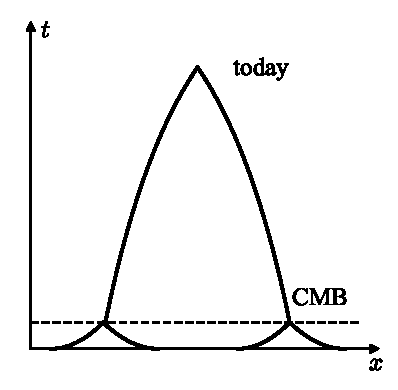
\includegraphics[width=0.72\textwidth]{fig_8.7.pdf}
\caption*{图 8.7\quad 从一个由大爆炸奇点膨胀而来的宇宙中的过去光锥，展示了宇宙学中的粒子视界。处于复合时刻的一些点——今天作为天空中相反两侧的宇宙微波背景被我们观测到——其过去光锥互不重叠（在传统宇宙学中）；没有任何因果信号能够影响它们，使它们具有相同的温度。}
\end{figure}
记住 $a_{0}=1$。因此 Hubble 参量为
\begin{equation*}
\begin{aligned}
H &= \frac{2}{3}t^{-1} \\
&= a^{-3/2}H_{0}.
\end{aligned}
\tag{8.184}
\end{equation*}
于是该光子走过的共动距离为
\begin{equation*}
\Delta r = 2H_{0}^{-1}\left(\sqrt{a_{2}}-\sqrt{a_{1}}\right).
\tag{8.185}
\end{equation*}
在尺度因子取任一固定值 $a=a_{*}$ 时的共动视界尺度，是光子自大爆炸以来走过的距离，
\begin{equation*}
r_{\mathrm{hor}}(a_{*}) = 2H_{0}^{-1}\sqrt{a_{*}}.
\tag{8.186}
\end{equation*}
而在 $a_{*}$ 处的空间超曲面上测得的物理视界尺寸，因此就简单地是
\begin{equation*}
d_{\mathrm{hor}}(a_{*}) = a_{*}r_{\mathrm{hor}}(a_{*}) = 2H_{*}^{-1}.
\tag{8.187}
\end{equation*}
事实上，对任何包含物质和辐射混合物的近平直宇宙，在任一给定时期我们都有
\begin{equation*}
d_{\mathrm{hor}}(a_{*}) \sim H_{*}^{-1} = d_{H}(a_{*}),
\tag{8.188}
\end{equation*}

% ---- 书页 368 / p383 ----
其中 Hubble 距离 $d_{H}$ 已在式 (8.71) 中引入。这种近似相等带来一种强烈的诱惑，即把“视界距离”和“Hubble 距离”当作同义词使用；这种诱惑应当抵制，因为暴胀可以使前者远大于后者，我们很快就会证明这一点。

视界问题简单说来就是：CMB 在很高的精度上是各向同性的，尽管最后散射面上相距遥远的各点彼此完全处于对方的视界之外。当我们观看 CMB 时，我们观测的是尺度因子 $a_{\mathrm{CMB}}\approx 1/1200$ 处的宇宙；由式 (8.185)，CMB 上一点与地球上的观者之间的共动距离为
\begin{equation*}
\begin{aligned}
\Delta r &= 2H_{0}^{-1}\left(1-\sqrt{a_{\mathrm{CMB}}}\right) \\
&\approx 2H_{0}^{-1}.
\end{aligned}
\tag{8.189}
\end{equation*}
然而，这样一个点所对应的共动视界距离为
\begin{equation*}
\begin{aligned}
r_{\mathrm{hor}}(a_{\mathrm{CMB}}) &= 2H_{0}^{-1}\sqrt{a_{\mathrm{CMB}}} \\
&\approx 6\times 10^{-2}H_{0}^{-1}.
\end{aligned}
\tag{8.190}
\end{equation*}
因此，如果我们观测 CMB 中相距遥远的两个部分，它们的视界将互不重叠；CMB 天空中不同的斑块在复合时刻是因果不连通的。然而，观测却表明它们具有相同的温度，且精度很高。于是问题就来了：既然它们从未处于因果接触之中，它们是如何预先知道要以正确的方式协调各自的演化的？我们必须设法修正传统 FRW 宇宙学的因果结构。

让我们考虑这样修正传统图像：设定一段\textbf{暴胀}（inflation）时期，即极早期宇宙中一段加速膨胀（$\ddot{a}>0$）的时期，由物质或辐射以外的某种成分驱动，这种成分随宇宙膨胀而红移得很慢。这样一来，平坦性问题和视界问题便可以同时解决。为简单起见，考虑暴胀由恒定的真空能驱动、从而导致指数膨胀的情形。于是，在真空主导的时期，$\rho/3\bar{m}_{\mathrm{P}}^{2}\propto a^{0}$ 相对于 $-\kappa/a^{2}$ 迅速增大，宇宙随时间变得越来越平（$\Omega$ 被驱动到 1）。如果这个过程持续了足够长的时间，然后真空能才转化为物质和辐射，那么密度参数将足够接近 1，以至于进入当前时代之前它还来不及发生可察觉的改变。与此同时，视界问题可以追溯到这样一个事实：任意两个共动物体之间的物理距离随尺度因子增长，而物质主导或辐射主导宇宙中的物理视界尺寸增长得更快，$d_{\mathrm{hor}}\sim a^{n/2}H_{0}^{-1}$。这同样可以由早期一段指数膨胀时期来解决：真实的视界尺寸会增长到一个惊人的数量，以至于我们今天的视界实际上远大于“视界等于 Hubble 半径 $H_{0}^{-1}$”这个天真的估计。

事实上，真正的指数膨胀并非必需；对任何加速膨胀，空间曲率相对于能量密度都会减小，
% ---- 书页 369 / p384 ----
而视界距离将迅速增长。通常我们要求这个加速时期持续 60 个或更多的 $e$ 指数倍（e-fold，$e$ 指数倍数为 $N=\Delta\ln a$），这正是解决视界问题所需要的。很容易做过头，暴胀一般会使今天的宇宙在空间上平直得难以置信。

现在让我们考虑如何在早期宇宙中得到一个暴胀阶段。最直接的办法是利用一个标量场的势所提供的真空能，这个场就是\textbf{暴胀子}（inflaton）。想象一个由空间均匀的标量（场）的能量主导的宇宙。相关的运动方程正是我们在 8.7 节中讨论动力学暗能量时的那些方程；唯一的区别是暴胀的能量标度要高得多。我们有 RW 度规中标量场的运动方程，
\begin{equation*}
\ddot{\phi} + 3H\dot{\phi} + V'(\phi) = 0,
\tag{8.191}
\end{equation*}
以及弗里德曼方程
\begin{equation*}
H^{2} = \frac{1}{3\bar{m}_{\mathrm{P}}^{2}}\left(\frac{1}{2}\dot{\phi}^{2} + V(\phi)\right).
\tag{8.192}
\end{equation*}
我们忽略了曲率项，因为暴胀反正会把宇宙拉平。如果场的演化足够平缓，使势能得以主导动能，并且 $\phi$ 的二阶导数足够小，足以让这种状态维持一段充分长的时间，暴胀就能发生。因此，我们希望
\begin{equation*}
\begin{aligned}
\dot{\phi}^{2} &\ll V(\phi), \\
|\ddot{\phi}| &\ll |3H\dot{\phi}|,\ |V'|.
\end{aligned}
\tag{8.193}
\end{equation*}
满足这些条件要求两个无量纲量足够小，它们就是所谓的\textbf{缓慢滚动参数}（slow-roll parameters）：
\begin{equation*}
\begin{aligned}
\epsilon &= \frac{1}{2}\bar{m}_{\mathrm{P}}^{2}\left(\frac{V'}{V}\right)^{2}, \\
\eta &= \bar{m}_{\mathrm{P}}^{2}\left(\frac{V''}{V}\right).
\end{aligned}
\tag{8.194}
\end{equation*}
注意 $\epsilon\ge 0$，而 $\eta$ 可正可负。还要注意，这些定义并非人人通用；有些人喜欢用 Hubble 参量而不是势来定义它们。我们的选择描述的是场是否有机会缓慢滚动一阵子；而用 Hubble 参量的描述给出的则是场实际上是否正在缓慢滚动。当这两个量都很小时，我们就可以有一个长久的暴胀阶段。然而它们并不充分；无论势是什么样子，我们总可以选取初始条件使 $|\dot{\phi}|$ 大到缓慢滚动永不适用。不过，只要缓慢滚动参数很小，大多数初始条件都会被吸引到暴胀阶段去。

% ---- 书页 370 / p385 ----
要发明满足缓慢滚动条件的势并不难。考虑也许是最简单的例子\footnote{我们沿用 A.R.~Liddle, \emph{An Introduction to Cosmological Inflation}（\texttt{http://arxiv.org/astro-ph/9901124}）中的讲述。}，$V(\phi)=\frac{1}{2}m^{2}\phi^{2}$。在这种情形下
\begin{equation*}
\epsilon = \eta = \frac{2\bar{m}_{\mathrm{P}}^{2}}{\phi^{2}}.
\tag{8.195}
\end{equation*}
显然，只要 $\phi$ 足够大，我们就能让缓慢滚动参数要多小有多小。然而，我们有一个约束：能量密度不应高达 Planck 标度，这样我们的经典分析才有意义；这意味着 $\phi\ll\bar{m}_{\mathrm{P}}^{2}/m$。如果我们把场从值 $\phi_{i}$ 开始，那么在暴胀结束之前（也就是缓慢滚动参数变成 1 的量级之前）的 $e$ 指数倍数将是
\begin{equation*}
\begin{aligned}
N &= \int_{t_{i}}^{t_{e}} H\,\mathrm{d}t \\
&\approx -\bar{m}_{\mathrm{P}}^{-2}\int_{\phi_{i}}^{\phi_{e}}\frac{V}{V'}\,\mathrm{d}\phi \\
&\approx \frac{\phi_{i}^{2}}{4\bar{m}_{\mathrm{P}}^{2}} - \frac{1}{2}.
\end{aligned}
\tag{8.196}
\end{equation*}
第一个等式总是成立，第二个等式用了缓慢滚动近似，第三个等式是这个具体模型的结果。要得到 60 个 $e$ 指数倍，我们需要 $\phi_{i}>16\bar{m}_{\mathrm{P}}$。再加上能量密度的上限，我们发现质量参数存在一个上限：$m\ll\bar{m}_{\mathrm{P}}/16$。事实上，观测到的密度涨落的大小对 $m$ 给出了更严格的上限，我们将在下面讨论。但 $m$ 没有下限，因此，只有当我们愿意设定 $m\ll\bar{m}_{\mathrm{P}}$ 这样的巨大层级差，或者等价地一个很小的无量纲数 $m/\bar{m}_{\mathrm{P}}$ 时，才容易得到合适的暴胀势。用 $\lambda\phi^{4}$ 势做同样的练习也会得出类似的结论：$\lambda$ 必须相当小；我们常说暴胀子必须是弱耦合的。当然，从某种意义上说这是在作弊，因为当场值 $\phi>\bar{m}_{\mathrm{P}}$ 时，我们应当预期有效势中会出现形如 $\bar{m}_{\mathrm{P}}^{4-n}\phi^{n}$（$n>4$）的附加项并变得重要。所以在一个\emph{现实}的模型中，要得到合适的势可能相当困难。

暴胀终会在某个时刻结束，暴胀子势中的能量将转化为物质和辐射的热化气体，这个过程被称为“再热”（reheating）。恰当地理解再热过程至关重要，因为它控制着我们宇宙中种种我们想要或不想要的遗留物（relic）的产生。例如，暴胀的一个重要好处是，它能够把早期宇宙中可能产生、但今天并未观测到的各种遗留物“暴胀掉”（inflate away）。一个经典的例子出现在粒子物理大统一理论的语境中：大统一理论一般预言存在超重的磁单极子，其丰度比观测容许的还要多出许多个数量级。

% ---- 书页 371 / p386 ----
历史上，磁单极子问题是 Guth 发明暴胀的首要动机；平坦性问题和视界问题的解决当时被视为额外的红利。暴胀可以把磁单极子的丰度稀释到合适的程度，但如果宇宙再热到超过大统一相变的温度，它们又会重新产生；幸运的是，对大多数模型而言这并不是一个严格的约束。类似的考虑也适用于其他不想要的遗留物；在超对称模型中，引力微子（gravitino，引力子的超对称伙伴）的丰度引起一个尤其令人头疼的问题。与此同时，又必须再热到足够高的温度，以便某种重子生成方案得以进行。对于在某个粒子物理模型内实现暴胀的任何具体方案，关键的检查是：不想要的遗留物被清除，而想要的遗留物（例如重子）得以保留。

暴胀方案的一个关键要素是密度微扰的产生，它们可能是我们今天观测到的 CMB 温度各向异性和星系大尺度结构的起源。暴胀产生密度微扰背后的想法相当直截了当。暴胀会把任何环境粒子密度迅速衰减到零，只留下真空。但是加速宇宙中的真空态具有非零的温度，即 Gibbons--Hawking 温度，它类似于黑洞的 Hawking 温度。我们无法在本书中深入探讨这个主题；这里只概述其基本结果。

对于一个由势能 $V$ 主导的宇宙，Gibbons--Hawking 温度为
\begin{equation*}
T_{\mathrm{GH}} = \frac{H}{2\pi} \sim \frac{V^{1/2}}{\bar{m}_{\mathrm{P}}}.
\tag{8.197}
\end{equation*}
与这个温度相对应的，是暴胀子场 $\phi$ 在每个波数 $k$ 处的涨落，其大小为
\begin{equation*}
|\Delta\phi|_{k} = T_{\mathrm{GH}}.
\tag{8.198}
\end{equation*}
由于势按假设近乎平坦，$\phi$ 的涨落会导致能量密度的小涨落，
\begin{equation*}
\delta\rho = V'(\phi)\delta\phi.
\tag{8.199}
\end{equation*}
因此，暴胀在所有尺度上都产生密度微扰。微扰的幅度在每个波数处都几乎相等，但由于暴胀子滚动时 $V$ 的逐渐变化，会有微小的偏离。描述这些微扰是一个繁乱的课题，涉及数不清的各种记号。一个合理的出发点是方均根（root-mean-square，RMS）密度涨落，
\begin{equation*}
\left.\frac{\delta\rho}{\rho}\right|_{\mathrm{rms}} = \sqrt{\left\langle\left(\frac{\delta\rho}{\rho}\right)^{2}\right\rangle},
\tag{8.200}
\end{equation*}

% ---- 书页 372 / p387 ----
其中尖括号表示对空间位置的平均。对于统计各向同性的微扰（期望幅度与方向无关），稍稍做一点傅里叶分析便能让我们写出
\begin{equation*}
\left(\left.\frac{\delta\rho}{\rho}\right|_{\mathrm{rms}}\right)^{2} = \int \Delta^{2}(k)\,\mathrm{d}(\ln k),
\tag{8.201}
\end{equation*}
其中我们引入了无量纲功率谱，
\begin{equation*}
\Delta^{2}(k) \equiv \frac{k^{3}|\delta_{k}|^{2}}{2\pi^{2}},
\tag{8.202}
\end{equation*}
而 $\delta_{k}$ 是分数密度微扰（fractional density perturbation）的傅里叶变换的期望值，
\begin{equation*}
\delta_{\mathbf{k}} = \frac{1}{(2\pi)^{3/2}}\int e^{-i\mathbf{k}\cdot\mathbf{x}}\frac{\delta\rho}{\rho}\,\mathrm{d}^{3}x,
\tag{8.203}
\end{equation*}
这里我们已假设它是各向同性的。无量纲功率谱是时间的函数，因为每个模式的幅度都在演化；表达任何具体模型的预言时，最常用的做法是取模式的物理波长 $\lambda=a/k$ 等于 Hubble 半径 $H^{-1}$ 的那一时刻的微扰幅度，
\begin{equation*}
A_{S}^{2}(k) \equiv \left.\Delta^{2}(k)\right|_{k=aH}.
\tag{8.204}
\end{equation*}
这样，$A_{S}(k)$ 量度的是不同模式在不同时刻的幅度。对于由缓慢滚动标量场驱动的暴胀，$A_{S}(k)$ 与势通过下式相联系：
\begin{equation*}
A_{S}^{2}(k) \sim \left.\frac{V^{3}}{\bar{m}_{\mathrm{P}}^{6}(V')^{2}}\right|_{k=aH} \sim \left.\frac{V}{\bar{m}_{\mathrm{P}}^{4}\epsilon}\right|_{k=aH}.
\tag{8.205}
\end{equation*}
我们有意略去了无量纲的数值因子——它们在不同文献之间差别很大——以便突出对势的依赖。

谱带着下标“S”，是因为它描述的是度规中的标量涨落。这些涨落与能量-动量分布绑定在一起，暴胀产生的密度涨落是绝热的——所有物种的密度涨落都是相互关联的。涨落还是高斯的，其含义是：描述不同尺度上涨落的那些傅里叶模式的相位互不相关。暴胀微扰的这些方面——近无标度的绝热密度涨落谱、高斯分布——都与当前对 CMB 和大尺度结构的观测一致，而今后几年预定要收集的新数据应会大大提高这些检验的精度。

% ---- 书页 373 / p388 ----
在暴胀期间被激发的不仅是近无质量的暴胀子，还有任何其他近无质量的粒子。另一个重要的例子是引力子，它对应于度规中的张量微扰（引力场的传播激发）。张量涨落具有谱
\begin{equation*}
A_{T}^{2}(k) \sim \left.\frac{V}{\bar{m}_{\mathrm{P}}^{4}}\right|_{k=aH}.
\tag{8.206}
\end{equation*}
重要的是，张量幅度只依赖于势本身，而不依赖于它的导数；因此，对张量微扰的观测将直接给出关于暴胀能量标度的信息。

为了理解观测，用可观测的量来参数化微扰谱是有用的。于是我们写出
\begin{equation*}
A_{S}^{2}(k) \propto k^{n_{S}-1}
\tag{8.207}
\end{equation*}
以及
\begin{equation*}
A_{T}^{2}(k) \propto k^{n_{T}},
\tag{8.208}
\end{equation*}
其中 $n_{S}$ 和 $n_{T}$ 是谱指数（spectral index）。它们与势的缓慢滚动参数的关系为
\begin{equation*}
n_{S} = 1 - 6\epsilon + 2\eta
\tag{8.209}
\end{equation*}
以及
\begin{equation*}
n_{T} = -2\epsilon.
\tag{8.210}
\end{equation*}
在我们所考虑的这类模型（由单个缓慢滚动的标量场驱动）中，存在一个把标量模式和张量模式的幅度与谱指数联系起来的自洽关系。它可以用一种与约定无关的方式表达为可观测量之间的关系，即不同微扰所导致的温度涨落 $\Delta T$ 之间的关系：
\begin{equation*}
\frac{(\Delta T/T)_{T}^{2}}{(\Delta T/T)_{S}^{2}} = -7n_{T}.
\tag{8.211}
\end{equation*}

张量微扰的存在是暴胀的一个关键预言，原则上可以通过对 CMB 偏振的观测加以检验。偏振也可以由通常的密度涨落诱导产生，其机制是非均匀等离子体中 Thompson 散射截面的各向异性。幸运的是，我们可以设想把天空中的偏振矢量场分解为无旋部分（$E$ 模式）和有旋部分（$B$ 模式）；标量微扰导致 $E$ 模式偏振，而张量微扰导致 $B$ 模式（除去复合之后的宇宙中某些不可避免的演化加工）。CMB 偏振已经被探测到了；未来的挑战将在于把标量和张量的贡献分离出来，以检验简单暴胀模型的预言 (8.211)。

% ---- 书页 374 / p389 ----
当然，这不仅要求探测到张量诱导的偏振，还要求以一定的精度测量它的谱指数。

我们对微扰幅度已有的知识，已经给了我们关于暴胀能量标度的重要信息。张量微扰只依赖 $V$ 本身，不依赖它的导数；如果 COBE 观测到的 CMB 各向异性源自张量涨落（有可能，尽管不太可能），我们可以立刻导出 $V_{\mathrm{inflation}}\sim(10^{16}~\mathrm{GeV})^{4}$。这里，受到约束的 $V$ 值是产生观测涨落的那一时刻的值，即暴胀结束前 60 个 $e$ 指数倍时的值。这极其让人联想到大统一标度，十分令人鼓舞。即使在更可能的情形下——CMB 中观测到的微扰本质上是标量的——我们仍然可以写出
\begin{equation*}
V_{\mathrm{inflation}}^{1/4} \sim \epsilon^{1/4}10^{16}~\mathrm{GeV},
\tag{8.212}
\end{equation*}
其中 $\epsilon$ 是式 (8.194) 定义的缓慢滚动参数。虽然我们预期 $\epsilon$ 很小，但指数中的 $1/4$ 意味着对 $\epsilon$ 的依赖相当弱；除非这个参数小得出奇，否则很有可能 $V_{\mathrm{inflation}}^{1/4}\sim 10^{15}$--$10^{16}~\mathrm{GeV}$。我们能对如此惊人的能量标度获得这样的信息，这一事实本身就足以令人惊叹。

\section{习题}

\textbf{1.}\quad 考虑一个 $(N+n+1)$ 维时空，坐标为 $\{t,\,x^{I},\,y^{i}\}$，其中 $I$ 从 1 取到 $N$，$i$ 从 1 取到 $n$。设度规为
\begin{equation*}
\mathrm{d}s^{2} = -\mathrm{d}t^{2} + a^{2}(t)\delta_{IJ}\,\mathrm{d}x^{I}\mathrm{d}x^{J} + b^{2}(t)\gamma_{ij}(y)\,\mathrm{d}y^{i}\mathrm{d}y^{j},
\tag{8.213}
\end{equation*}
其中 $\delta_{IJ}$ 是通常的 Kronecker delta，而 $\gamma_{ij}(y)$ 是 $n$ 维最大对称空间流形上的度规。设想我们把度规 $\gamma$ 归一化，使得曲率参数
\begin{equation*}
k = \frac{R(\gamma)}{n(n-1)}
\tag{8.214}
\end{equation*}
等于 $+1$、$0$ 或 $-1$，其中 $R(\gamma)$ 是度规 $\gamma_{ij}$ 所对应的 Ricci 标量。

\textbf{(a)}\quad 计算这个度规的 Ricci 张量。

\textbf{(b)}\quad 用能量密度 $\rho$ 以及 $x^{I}$ 和 $y^{i}$ 方向上的压强 $p^{(N)}$、$p^{(n)}$ 定义一个能量-动量张量：
\begin{gather*}
T_{00} = \rho \tag{8.215}\\
T_{IJ} = a^{2}p^{(N)}\delta_{IJ} \tag{8.216}\\
T_{ij} = b^{2}p^{(n)}\gamma_{ij}. \tag{8.217}
\end{gather*}
把这个度规和 $T_{\mu\nu}$ 代入 Einstein 方程，推导 $a$ 和 $b$ 所满足的类弗里德曼方程（共三个独立方程）。

% ---- 书页 375 / p390 ----
\textbf{(c)}\quad 推导静态解（即 $\dot{a}=\dot{b}=\ddot{a}=\ddot{b}=0$ 的解）处能量密度和两个压强所满足的方程，用 $k$、$n$ 和 $N$ 表示。利用它们推导物态方程参数 $w^{(N)}=p^{(N)}/\rho$ 和 $w^{(n)}=p^{(n)}/\rho$ 在静态解处成立的表达式。

\textbf{2.}\quad 考虑 de Sitter 空间，采用度规取如下形式的坐标：
\begin{equation*}
\mathrm{d}s^{2} = -\mathrm{d}t^{2} + e^{2Ht}\left[\mathrm{d}x^{2}+\mathrm{d}y^{2}+\mathrm{d}z^{2}\right].
\tag{8.218}
\end{equation*}
对非共动观者（$x^{i}$ 不是常数）求解测地线方程，求出作为 $t$ 的函数的仿射参量。证明测地线在有限的仿射参量内到达 $t=-\infty$，从而证明这些坐标不能覆盖整个流形。

\textbf{3.}\quad 在附录 F 中我们讨论了 Raychaudhuri 方程。证明：把它应用到 Robertson--Walker 宇宙学上，Raychaudhuri 方程等价于第二弗里德曼方程 (8.68)。

\textbf{4.}\quad 考虑最佳拟合宇宙，其密度参数为 $\Omega_{\mathrm{R}0}=10^{-4}$、$\Omega_{\mathrm{M}0}=0.3$、$\Omega_{\Lambda0}=0.7$。在对数标度上画出三个 $\Omega_{i}$ 作为尺度因子 $a$ 的函数的图像，$a$ 从 $10^{-35}$ 取到 $10^{35}$。标出 Planck 时间、核合成和今天。

\textbf{5.}\quad 在平直时空中，物理尺寸固定的物体离得越远，所张的角就越小；在膨胀宇宙中未必如此。考虑红移 $z$ 处物理尺寸为 $L$ 的物体的角大小 $\theta(z)$。在物质主导的平直宇宙中，$\theta(z)/L$ 在什么红移处取极小？如果所有星系的跨度都至少有 $10~\mathrm{kpc}$（并且历来如此），这样一个宇宙中星系的最小角大小是多少？把你的结果既用 $H_{0}$ 表示，也代入 $H_{0}=70~\mathrm{km/s/Mpc}$ 给出数值。

\textbf{6.}\quad 在宇宙学中，我们倾向于把非相对论性粒子理想化为温度 $T$ 和压强 $p$ 都为零。实际上，随机运动会使它们具有一定的温度和压强，满足 $p\propto T\rho$。

\textbf{(a)}\quad 由有质量粒子组成的气体，其压强作为尺度因子的函数会如何衰减？

\textbf{(b)}\quad 设中微子具有质量 $m_{\nu}=0.1~\mathrm{eV}$，当前温度为 $T_{\nu 0}=2~\mathrm{K}$。中微子大约在什么红移从相对论性变为非相对论性？

\textbf{7.}\quad 设想宇宙在 Planck 时刻以均分状态（equipartition）出发（这样物质和辐射中的能量密度为 Planck 密度的量级，时间与空间的曲率半径为 Planck 长度的量级）。忽略任何空间不均匀性，计算一个正曲率宇宙能维持多久，以及一个负曲率宇宙在温度降到 $3~\mathrm{K}$ 时年龄多大。一个平直宇宙在温度降到 $3~\mathrm{K}$ 时年龄多大？一个平直宇宙到膨胀速率降至 $H_{0}=70~\mathrm{km\,s^{-1}\,Mpc^{-1}}$ 时年龄多大？

 % 本文件由 scripts/assemble.py 自动装配，勿手改（改 parts/ 后重跑）
% 第9章 弯曲时空量子场论

% 第9章 Quantum Field Theory in Curved Spacetime
\chapter{弯曲时空量子场论}

\section{引言}

% ---- 书页 376 / p391 ----
没有人相信，就引力而言广义相对论就是最终的定论。奇点定理从理论内部提供了证据，表明这个理论在某种意义上是不完备的；然而更有说服力的是这样一个事实：广义相对论是一个经典理论，而世界在根本上是量子力学的。寻找一个能实际运作的量子引力理论，驱动着当今理论物理中的大量研究，这一路上我们也确实学到了许多，但令人信服的成功始终遥不可及。

广义相对论有两个组成部分：其一是时空曲率的框架及其对物质的影响，其二是度规响应能量-动量的动力学（由 Einstein 方程描述）。虽然还没有一个真正的量子引力理论，我们仍然可以取广义相对论的前一部分——物质场在弯曲时空背景上传播这一观念——并考虑那些物质场本身是量子力学的情况。换句话说，我们把度规取为固定的，而不让它服从什么动力学方程，然后研究这个弯曲时空中的量子场论（quantum field theory，QFT）。

弯曲时空量子场论研究中的划时代事件，是 Hawking 在 1976 年认识到黑洞其实并不真的黑，而是会发出热辐射，其温度是一个正比于表面引力（surface gravity）$\kappa$ 的\textbf{Hawking 温度}（Hawking temperature），
\begin{equation*}
\boxed{\;T = \frac{\kappa}{2\pi}.\;}\tag{9.1}
\end{equation*}
（回忆一下，我们的单位制取 $\hbar = c = k = 1$；Hawking 温度实际上正比于 $\hbar$，并反比于 Boltzmann 常数 $k$。）自这一非凡的发现以来，弯曲时空量子场论已被置于相当严格的理论基础之上，尽管人们普遍认为，它的适用范围离任何可能的实验探测都还相当遥远。Schwarzschild 黑洞的表面引力为 $\kappa = 1/4GM$，其 Hawking 温度可以写成
\begin{equation*}
T = \frac{1}{8\pi GM} = 1.2\times 10^{26}\,K\left(\frac{1\,\mathrm{g}}{M}\right) = 6.0\times 10^{-8}\,K\left(\frac{M_\odot}{M}\right),
\tag{9.2}
\end{equation*}
其中 $M_\odot \sim 10^{33}$ g 是太阳的质量。因此，来自一个现实的天体物理黑洞的辐射，其温度甚至比 3K 的宇宙微波背景还要低得多，因而基本上毫无被观测到的希望。

% ---- 书页 377 / p392 ----
然而，近来宇宙学方面的观测在某种程度上改变了这一局面。一个例子是看似发现了宇宙正在加速，这一结果最容易解释为非零真空能（vacuum energy）的证据（如第 8 章所讨论）。虽然真空能的大小仍然是一个深刻的谜，但有一点似乎是清楚的：理解量子力学的物质在弯曲时空中如何行为，将在任何对这一谜题的最终解决中扮演重要角色。另一个例子来自宇宙学扰动。对微波背景和大尺度结构的观测，为原初扰动的近无标度谱提供了强有力的证据，其中包括那些波长将远大于常规宇宙学中视界尺度的扰动。关于这些扰动起源的领先理论来自暴胀（inflation）。在暴胀场景中，宇宙学扰动起源于正在暴胀的宇宙中量子场的真空涨落。如果这幅图像是正确的，那么我们在 CMB 图中看到的，就是原初量子涨落被宇宙的膨胀大大拉伸之后留下的印记，而正是这些涨落经由引力不稳定性最终成长为今天我们所看到的星系和星系团。因此，至少可以说，宇宙学观测为弯曲时空量子场论的研究提供了强有力的动机。

即使没有这种经验上的动机，基于弯曲时空量子场论的思想实验，也已经在我们对量子引力的试探性探索中被证明是非常富有成果的。特别是，霍金辐射所预言的黑洞蒸发导致了信息丢失佯谬（information-loss paradox），我们将在下文讨论。由于直接触及量子引力问题的真实实验是如此困难，我们必须依靠聚焦于广义相对论与量子力学之间张力的思想实验，这很像 Einstein 当年试图调和经典动力学与电磁学的洛伦兹不变性时所用的思想实验。

带着这些考虑，本章的目标是对弯曲时空量子场论的一些观念和结果作一个简要的介绍。许多广义相对论入门书不讲这个主题，通常是因为学习广义相对论不应以熟悉平直时空中的普通量子场论为先决条件。然而令人愉快的事实是：熟悉平直时空中的量子场论，对于学习弯曲时空中的量子场论完全不是必需的。这是因为，在平直时空中最有趣、最有用的那些量子场论特征，与在弯曲时空中有趣、有用的那些特征几乎完全不同。往深处说，量子场论不过是量子力学系统的一个例子，就同方势阱或氦原子一样。一旦定义了一个场论，它在平直时空中的应用（对粒子物理或凝聚态物质）自然会聚焦于各种场之间相互作用的问题，通常把相互作用处理成围绕某个自然真空态的微扰。然而在弯曲时空中，我们感兴趣的通常是时空本身对场的影响，对此相互作用根本不是要点。因此我们可以考虑自由（无相互作用）场，但我们必须格外小心地定义什么才是合适的真空态。（的确，正如我们将要看到的，我们与之打交道的态几乎全都是真空态！）其结果是，平直时空量子场论的知识对眼下的讨论不仅不必要，甚至可能帮不上什么忙；唯一的先决条件是熟悉普通量子力学的基础。

% ---- 书页 378 / p393 ----
我们将循序渐进地走向弯曲时空中的量子场论，从复习这样一个系统的量子力学开始——每个物理学家在遇到棘手问题时都会求助于它：简谐振子（simple harmonic oscillator）。这当然是量子力学原理如何运作的一个典范性例子，而且还有一个额外的好处：当我们接下来转向场论时会发现，平直时空中自由场的量子力学恰好就是无穷多个谐振子的量子力学。（并不是空间每一点上都有一个振子，而是场的傅里叶变换中的每一个模式都表现得像一个谐振子。）于是，从谐振子到场论的过渡相当直截了当。一旦掌握了场论的基础，鉴于我们先前对广义相对论的学习，推广到弯曲时空并不十分困难，尽管沿途会遇到不少微妙之处。我们的讨论必然有些浅尝辄止，重心放在这样一个目标上：通过理解平直时空中的安鲁效应（Unruh effect）来理解霍金辐射的物理基础。特别是，我们不会讨论弯曲时空量子场论在宇宙学中的重要应用，也不会深入细致地考察重整化及相关问题。我们在很大程度上遵循 Birrell and Davies (1982) 的讨论；欲作进一步的探究，可查阅该书、Wald (1994)，或 Ford\footnote{L. H. Ford, “Quantum field theory in curved spacetime,” (1997), \texttt{http://arxiv.org/gr-qc/9707062}。} 的综述。

\section{量子力学}

量子场论只不过是量子力学系统的一个特定例子，所以我们可以从提醒自己这意味着什么开始。当然，尽管世界在根本上是量子力学的，我们的直觉却更容易同经典物理对上号，所以让我们先通过思考经典力学来搭好舞台。任何描述某个特定系统的物理理论，无论经典的还是量子的，都由以下三个问题的答案构成：

\begin{enumerate}
\item 系统的可能态是什么？在经典力学中，态空间通常由一组坐标和动量给出（我们可以把它们看作系统的“初始条件”）。它们可以被精确地指定，而这就是关于系统状态所要知道的一切。
\item 关于这个系统能观测到什么？这个问题在经典力学中往往只是隐含地处理，因为答案平淡无奇：坐标和动量的任何函数都有资格作为一个可观测量（observable）。
\item 系统如何演化？这通常由一组运动方程来表达。给定态和运动方程，随后的演化就唯一地确定了；于是，初始条件的空间就等价于该理论的经典解的空间。
\end{enumerate}

% ---- 书页 379 / p394 ----
为了让这些观念更具体，同时也因为它与我们研究场论直接相关，我们来考虑简谐振子。简谐振子可以想象成一维中受二次势作用的粒子。态由单个坐标 $x$ 和单个动量 $p$ 指定。为了得到运动方程，我们可以从拉格朗日量出发，它用 $x$ 及其时间导数 $\dot{x}$ 写成
\begin{equation*}
L = \frac{1}{2}\dot{x}^2 - \frac{1}{2}\omega^2 x^2,
\tag{9.3}
\end{equation*}
其中为方便起见，我们把振子的质量取为 1。我们可以立即导出运动方程
\begin{equation*}
\ddot{x} + \omega^2 x = 0.
\tag{9.4}
\end{equation*}
然而，为了过渡到量子力学，用哈密顿量来工作更加方便，它是 $x$ 和 $p$（而非 $x$ 和 $\dot{x}$）的函数。哈密顿量通过勒让德变换（Legendre transformation）与拉格朗日量相联系，
\begin{equation*}
H = p\dot{x} - L,
\tag{9.5}
\end{equation*}
其中动量满足
\begin{equation*}
p = \frac{\partial L}{\partial \dot{x}} = \dot{x}.
\tag{9.6}
\end{equation*}
于是我们得到振子的哈密顿量，
\begin{equation*}
H = \frac{1}{2}p^2 + \frac{1}{2}\omega^2 x^2,
\tag{9.7}
\end{equation*}
以及哈密顿方程
\begin{equation*}
\frac{dx}{dt} = \partial_p H = p, \qquad \frac{dp}{dt} = -\partial_x H = -\omega^2 x,
\tag{9.8}
\end{equation*}
它们充当运动方程。这些解当然是直截了当的；把它们表示成复数很有用：
\begin{equation*}
x(t) = x_0\, e^{i(\omega t + \alpha_0)},
\tag{9.9}
\end{equation*}
其中 $x_0$ 是振幅，$\alpha_0$ 是相位。到最后我们取实部，就得到物理答案。

现在我们转向量子力学。虽然量子力学与经典力学有着深刻的不同，但一个给定的理论仍然由与上面所列相同的三个问题的答案构成，只不过答案采取了多少有些不同的形式。

% ---- 书页 380 / p395 ----
\begin{enumerate}
\item 系统的态表示为\textbf{希尔伯特空间}（Hilbert space）中的一个元素。在数学上，希尔伯特空间就是一个装备了复数值内积的复矢量空间，该内积具有如下性质：以相反的次序取两个态的内积，等价于取复共轭。我们把希尔伯特空间的元素记作 $|\psi\rangle$，对偶空间的元素记作 $\langle\psi|$，于是 $|\psi_1\rangle$ 与 $|\psi_2\rangle$ 的内积就是 $\langle\psi_2|\psi_1\rangle$，并且满足
\begin{equation*}
\langle\psi_2|\psi_1\rangle^{*} = \langle\psi_1|\psi_2\rangle.
\tag{9.10}
\end{equation*}
（对于有关空间完备性的技术要求，我们在此不作深究。）在量子力学中，我们所感兴趣的希尔伯特空间往往都是无穷维的。例如，如果一个经典系统由坐标 $x$ 和动量 $p$ 来表示，那么希尔伯特空间可以取成由 $x$ 的所有平方可积复值函数组成，或者等价地由 $p$ 的所有平方可积复值函数组成（但不能同时取两者）。
\item 可观测量表示为希尔伯特空间上的\textbf{自伴算符}（self-adjoint operators）。“自伴”的定义实际上相当微妙，但在简单的情形下，它就相当于我们通常对厄米算符（Hermitian operator）的理解，
\begin{equation*}
A^{\dagger} = A,
\tag{9.11}
\end{equation*}
其中 $A^{\dagger}$ 满足
\begin{equation*}
\langle\psi_2|A\psi_1\rangle = \langle A^{\dagger}\psi_2|\psi_1\rangle
\tag{9.12}
\end{equation*}
对所有态 $|\psi_1\rangle$、$|\psi_2\rangle$ 成立。当然，许多算符并不是厄米的，但可观测量应当具有这一性质。一般说来，这类算符彼此不对易，因此我们无法同时精确地指明我们想要测量的关于系统的一切量的数值；将会存在一个对易可观测量完备集，它一次性地代表了我们对一个系统所能说的一切。
\item 系统的演化可以用两种方式之一来表示：或者作为希尔伯特空间中态矢量的幺正演化（\textbf{Schrödinger 绘景}，Schrödinger picture），或者保持态固定不动，而让可观测量按照运动方程演化（\textbf{Heisenberg 绘景}，Heisenberg picture）。
\end{enumerate}

严格说来，量子力学就是与经典力学不同；完全不必非得从一个经典模型出发，把它“量子化”。尽管如此，我们通常恰恰就是这么做的。即便是简单的经典模型，构造其量子化版本的方法也不止一种；其中包括正则量子化（canonical quantization）和路径积分量子化（path-integral quantization），以及一些更加奇特的手续。更糟的是，经典理论与量子理论之间并不存在简单的映射；有的经典理论没有良好定义的量子对应物，有的经典理论有好几个量子版本，还有的量子理论没有任何经典的类似物。就我们眼下的目的而言，我们可以对这些微妙之处满不在乎地一概置之不理，直接进行正则量子化。

% ---- 书页 381 / p396 ----
简谐振子再一次提供了一个有用的例子。先考虑大家熟悉的 Schrödinger 绘景，其中态由随时间演化的复值波函数表示，比如 $\psi(x,t)$。波函数实际上就是态矢量 $|\psi\rangle$ 的那一组分量，在“$\delta$ 函数位置基”$|x\rangle$ 中表出，于是 $|\psi(t)\rangle = \int dx\,\psi(x,t)|x\rangle$。正则量子化的内容就是加上正则对易关系（canonical commutation relation）
\begin{equation*}
[\hat{x}, \hat{p}] = i,
\tag{9.13}
\end{equation*}
把它加在坐标算符 $\hat{x}$ 及其共轭动量 $\hat{p}$ 上。对于由依赖 $x$ 和 $t$ 的波函数所表示的态，$\hat{x}$ 不过就是乘以 $x$，所以式 (9.13) 可以通过令
\begin{equation*}
\hat{p} = -i\partial_x.
\tag{9.14}
\end{equation*}
来实现。哈密顿算符是
\begin{equation*}
H = -\frac{1}{2}\partial_x^2 + \frac{1}{2}\omega^2 x^2,
\tag{9.15}
\end{equation*}
而运动方程就是 Schrödinger 方程，
\begin{equation*}
H\psi = i\partial_t\psi.
\tag{9.16}
\end{equation*}
由于哈密顿量不含时间，这个方程的解可以分离成空间的函数与时间的函数，$\psi(x,t) = f(t)g(x)$。这些解构成一个由整数 $n \geq 0$ 标记的离散集合，我们求得（在相差归一化因子的意义下）
\begin{equation*}
\psi_n(x,t) = e^{-(1/2)\omega x^2} H_n(\sqrt{\omega}\,x)\, e^{-iE_n t},
\tag{9.17}
\end{equation*}
其中 $H_n$ 是 $n$ 次厄米多项式（Hermite polynomial），而
\begin{equation*}
E_n = \left(n + \frac{1}{2}\right)\omega.
\tag{9.18}
\end{equation*}
这些态都是 $H$ 的本征函数，$E_n$ 就是能量本征值。振子的任意态无非就是能量本征态的叠加，
\begin{equation*}
\psi(x,t) = \sum_n c_n \psi_n(x,t),
\tag{9.19}
\end{equation*}
其中诸系数 $c_n$ 适当归一化。

这个简短的概述已包含了量子力学振子的许多重要特征。能量本征态具有分立谱；这正是它被称作“量子”力学的原因（尽管找出具有连续谱的系统并不困难）。存在一个能量最低的基态，以及一组由各自能量本征值唯一标记的激发态。基态具有非零的能量，
\begin{equation*}
E_0 = \frac{1}{2}\omega,
\tag{9.20}
\end{equation*}
它有时被称为“零点”能（zero-point energy）。有趣的是，经典系统的最小能量本来会是零，对应于 $x = 0$、$p = 0$ 的粒子。量子的零点能可以追溯到 Heisenberg 不确定性原理：它不许我们同时在位置和动量上把一个态定域化；因此振子中总存在一个最低限度的“抖动”，导致非零的基态能量。另一方面，我们当然也可以选择去考察一个势由 $V(x) = \frac{1}{2}\omega^2 x^2 - \frac{1}{2}\omega$ 给出的振子；我们的分析将完全相同，只不过式 (9.18) 中的因子 $\frac{1}{2}$ 不再出现，而基态能量将会是零。量子力学并不坚持非要有非零的零点能，它只是把能量从经典值那里挪动了一下。

% ---- 书页 382 / p397 ----
求解简谐振子的另一种办法，是引进产生算符和湮灭算符 $\hat{a}^{\dagger}$ 与 $\hat{a}$（常称为升算符和降算符，raising and lowering operators），其定义为
\begin{equation*}
\hat{a} = \frac{1}{\sqrt{2\omega}}\left(\omega\hat{x} + i\hat{p}\right), \qquad \hat{a}^{\dagger} = \frac{1}{\sqrt{2\omega}}\left(\omega\hat{x} - i\hat{p}\right),
\tag{9.21}
\end{equation*}
于是
\begin{equation*}
\hat{x} = \frac{1}{\sqrt{2\omega}}(\hat{a} + \hat{a}^{\dagger}), \qquad \hat{p} = -i\sqrt{\frac{\omega}{2}}(\hat{a} - \hat{a}^{\dagger}).
\tag{9.22}
\end{equation*}
利用我们先前关于对易关系的表达式 (9.13) 和哈密顿量 (9.7)，我们可以容易地算出产生算符和湮灭算符的对易关系，
\begin{equation*}
[\hat{a}, \hat{a}^{\dagger}] = 1,
\tag{9.23}
\end{equation*}
以及哈密顿量的新表达式，
\begin{equation*}
H = \left(\hat{a}^{\dagger}\hat{a} + \frac{1}{2}\right)\omega.
\tag{9.24}
\end{equation*}
产生/湮灭算符与哈密顿量按如下方式对易：
\begin{align*}
[H, \hat{a}] &= -\omega\hat{a} \\
[H, \hat{a}^{\dagger}] &= \omega\hat{a}^{\dagger}.
\tag{9.25}
\end{align*}
把这个版本的哈密顿量与能量本征值 (9.18) 相比较，我们受到启发，定义一个粒子数算符（number operator）
\begin{equation*}
\hat{n} = \hat{a}^{\dagger}\hat{a}.
\tag{9.26}
\end{equation*}

% ---- 书页 383 / p398 ----
让我们想一想，为什么产生/湮灭算符和粒子数算符配得上这些名字。考虑粒子数算符的一个本征态 $|n\rangle$，
\begin{equation*}
\hat{n}|n\rangle = n|n\rangle,
\tag{9.27}
\end{equation*}
其中左边的 $\hat{n}$ 代表粒子数算符，而右边第一个 $n$ 代表实际的数 $n$。（这个公式是整个量子力学中最迷人的公式。）摆弄一下对易关系，容易证明
\begin{align*}
\hat{n}\hat{a}^{\dagger}|n\rangle &= (n+1)\hat{a}^{\dagger}|n\rangle \\
\hat{n}\hat{a}|n\rangle &= (n-1)\hat{a}|n\rangle.
\tag{9.28}
\end{align*}
这样，当 $\hat{a}^{\dagger}$ 作用在 $|n\rangle$ 上时，它给出 $\hat{n}$ 的另一个本征态，本征值升高了 1；而 $\hat{a}$ 给出本征值降低了 1 的本征态。和前面一样，我们可以证明 $n$ 取从 $0$ 到 $\infty$ 的整数值，因此必定存在一个真空态 $|0\rangle$，满足
\begin{equation*}
\hat{a}|0\rangle = 0.
\tag{9.29}
\end{equation*}
从这个态出发，借助产生算符的逐次作用，我们可以构造出所有的本征态，
\begin{equation*}
|n\rangle = \frac{1}{\sqrt{n!}}\left(\hat{a}^{\dagger}\right)^{n}|0\rangle.
\tag{9.30}
\end{equation*}
粒子数算符计数的是高出基态的激发的数目。本征态的集合 $|n\rangle$ 充当一组基；任何态都是这些态的适当线性组合。产生算符和湮灭算符按如下方式作用在它们之上：
\begin{align*}
\hat{a}|n\rangle &= \sqrt{n}\,|n-1\rangle \\
\hat{a}^{\dagger}|n\rangle &= \sqrt{n+1}\,|n+1\rangle,
\tag{9.31}
\end{align*}
而每个态的能量当然由式 (9.18) 给出。基矢态取为不含时间，于是，一个服从 Schrödinger 方程的物理系统将用态
\begin{equation*}
|\psi(t)\rangle = \sum_n c_n e^{-iE_n t}|n\rangle,
\tag{9.32}
\end{equation*}
来描述，其中诸 $c_n$ 同样是常数系数。

为了让向场论的过渡更加平滑，把这种 Schrödinger 绘景的描述转译成 Heisenberg 绘景是有用的，在 Heisenberg 绘景中态是固定的，算符则随时间演化。给定 Schrödinger 方程 (9.16)，任何态都可以形式地写成某个固定的初始态经一个幺正时间演化算符作用后的结果，
\begin{equation*}
|\psi(t)\rangle = U(t)|\psi(0)\rangle,
\tag{9.33}
\end{equation*}

% ---- 书页 384 / p399 ----
其中
\begin{equation*}
U(t) = \mathcal{P}\, e^{-i\int H\,dt},
\tag{9.34}
\end{equation*}
（幺正的意思是 $U^{\dagger}U = 1$。）符号 $\mathcal{P}$ 代表路径排序（path-ordering），如附录 I 中所讨论。当然，如果哈密顿量不含时间，我们就简单地有 $U(t) = e^{-iHt}$。一个不含时算符 $A$ 在两个含时态 $|\psi_1(t)\rangle$ 和 $|\psi_2(t)\rangle$ 之间矩阵元的 Schrödinger 绘景表达式，于是可以写成 Heisenberg 绘景的表达式，即用含时算符 $A(t)$ 与不含时态表示为
\begin{align*}
\langle\psi_2(t)|A|\psi_1(t)\rangle &= \langle\psi_2(0)|U^{\dagger}(t)AU(t)|\psi_1(0)\rangle \\
&= \langle\psi_2|A(t)|\psi_1\rangle,
\tag{9.35}
\end{align*}
显然，其中 Heisenberg 绘景的算符由下式给出：
\begin{equation*}
A(t) = U^{\dagger}(t)AU(t).
\tag{9.36}
\end{equation*}
这样的算符满足\textbf{Heisenberg 运动方程}（Heisenberg equation of motion），
\begin{equation*}
\frac{dA(t)}{dt} = i[H, A(t)],
\tag{9.37}
\end{equation*}
它在这个绘景中取代了 Schrödinger 方程的位置。对于谐振子，我们会发现
\begin{equation*}
\frac{d\hat{a}}{dt} = -i\omega\hat{a}, \qquad \frac{d\hat{a}^{\dagger}}{dt} = i\omega\hat{a}^{\dagger},
\tag{9.38}
\end{equation*}
其解为
\begin{equation*}
\hat{a}(t) = e^{-i\omega t}\hat{a}(0), \qquad \hat{a}(t)^{\dagger} = e^{i\omega t}\hat{a}(0)^{\dagger}.
\tag{9.39}
\end{equation*}
由此我们立即得到
\begin{equation*}
\hat{n}(t) = \hat{a}(t)^{\dagger}\hat{a}(t) = \hat{a}(0)^{\dagger}\hat{a}(0),
\tag{9.40}
\end{equation*}
这反映了粒子数算符守恒这一事实。

人们常说，在 Heisenberg 绘景中态是不含时的；这话尽管不假，却有些令人困惑。或许更好的说法是：态延伸贯穿于整个时间，而不只是定义在某个固定时刻。为了把这一点看得更清楚，考虑一个受到外界影响的简谐振子，比如简单地在哈密顿量中加上一个强迫项，
\begin{equation*}
H = \frac{1}{2}p^2 + \frac{1}{2}\omega^2 x^2 + F(t),
\tag{9.41}
\end{equation*}
其中函数 $F(t)$ 在某个区间之外为零：
\begin{equation*}
F(t) =
\begin{cases}
0 & t < t_1 \\
F(t) & t_1 \leq t \leq t_2 \\
0 & t_2 < t .
\end{cases}
\tag{9.42}
\end{equation*}

% ---- 书页 385 / p400 ----
我们可以想象有人走过来，把我们的振子摇晃了一小会儿，然后就撒手不管了。在 Schrödinger 绘景中，我们会说：开始时处于基态的振子会被外力激发，末态不再是基态。而在 Heisenberg 绘景中，我们把态取成对所有时刻都成立的运动方程的解，并且说粒子数算符从零变成了某个别的值。

对于受到瞬态外力作用的振子，显然存在一组态，它们在早期看起来像能量本征态，尽管在将来就不再是这样了；我们可以把这样的态称为“in 态”$|n_{\mathrm{in}}\rangle$，它具有性质
\begin{equation*}
\hat{n}(t < t_1)|n_{\mathrm{in}}\rangle = n|n_{\mathrm{in}}\rangle.
\tag{9.43}
\end{equation*}
还有另外一组态，它们在晚期看起来像能量本征态，相应地称为“out 态”$|n_{\mathrm{out}}\rangle$，满足
\begin{equation*}
\hat{n}(t > t_2)|n_{\mathrm{out}}\rangle = n|n_{\mathrm{out}}\rangle.
\tag{9.44}
\end{equation*}
这两组态在所有时刻都存在，但只有在相应的渐近区域里，它们才看起来像能量本征态。任何一组都构成整个希尔伯特空间的一组基，所以特别地，我们可以用其中一组去展开另一组。例如，通过乘上一个 in 态的完备集，我们可以写出
\begin{equation*}
|n_{\mathrm{out}}\rangle = \sum_m \langle m_{\mathrm{in}}|n_{\mathrm{out}}\rangle|m_{\mathrm{in}}\rangle.
\tag{9.45}
\end{equation*}
复数 $\langle m_{\mathrm{in}}|n_{\mathrm{out}}\rangle$ 是矩阵元，原则上可以从哈密顿量 (9.41) 算出；它们合在一起构成\textbf{S 矩阵}（S-matrix）。一个装备了某种探测振子激发之手段的观者会发现，激发的数目被所施加的力改变了，而 S 矩阵编码了刻画渐近过去与渐近未来之间这些改变所需的全部信息。不用说，这整段讨论几乎可以原封不动地搬到场论中。在粒子物理里，外力的角色由不同粒子之间的相互作用扮演；而在我们的目的中，扮演这一角色的将是时空的曲率。

\section{平直时空中的量子场论}

正如我们已经提到的，量子场论只是量子力学系统的一个特定例子，其中被量子化的不是一个单个的振子，而是一个场（定义在时空上的一个函数，或者更一般地某个张量场）。我们从最简单的例子开始：平直时空中的自由标量场；从单个振子过渡到这个场论，只需再作寥寥几个推广。而把理论扩展到弯曲时空，照例是直截了当的：把理论写成协变形式，然后宣布它成立。然而，一旦失去了 Minkowski 空间的对称性，我们通常视为量子场论核心的一些观念就不再显得那么关键；特别是，“真空”与“粒子”的概念将失去它们的特权地位。（讲解量子力学的书偶尔会指出，波和粒子是适用范围各不相同的互补概念，但不要被误导；在量子场论中，真正基本的是场，而粒子只是在某些受限情形下才有用的近似概念。）本节我们先研究平直时空中的量子场论，下一节再推广到弯曲时空。

% ---- 书页 386 / p401 ----
我们从经典理论出发，具体说来是平直时空中的实标量场 $\phi(x^{\mu})$，正如我们在第 1 章中考虑过的那样，只是这次推广到 $n$ 维。作用量是拉格朗日密度（Lagrange density）的时空积分，$S = \int d^{\,n}x\,\mathcal{L}$；我们将考虑 Klein–Gordon 拉格朗日量
\begin{equation*}
\mathcal{L} = -\frac{1}{2}\eta^{\mu\nu}\partial_\mu\phi\,\partial_\nu\phi - \frac{1}{2}m^2\phi^2.
\tag{9.46}
\end{equation*}
没有必要纳入体积元因子 $\sqrt{|g|}$，因为我们在 Minkowski 空间中使用的是惯性坐标，其度规为
\begin{equation*}
ds^2 = -dt^2 + (d\mathbf{x})^2.
\tag{9.47}
\end{equation*}
运动方程是 Klein–Gordon 方程，
\begin{equation*}
\Box\phi - m^2\phi = 0.
\tag{9.48}
\end{equation*}
把场论转译成哈密顿描述是直截了当的。场的共轭动量（conjugate momentum）就是拉格朗日密度对该场的时间导数的导数，
\begin{equation*}
\pi = \frac{\partial\mathcal{L}}{\partial(\partial_0\phi)}.
\tag{9.49}
\end{equation*}
对于 Klein–Gordon 拉格朗日量 (9.46)，这就是
\begin{equation*}
\pi = \dot{\phi}.
\tag{9.50}
\end{equation*}
当然，一提到时间导数，就已默认我们选定了一个特定的惯性系；因此，哈密顿手续必然破坏显式的洛伦兹不变性。然而，只要我们足够小心，所得理论中的可观测量仍将是洛伦兹不变的。哈密顿量本身可以表示为哈密顿密度（Hamiltonian density）对空间的积分，
\begin{equation*}
H = \int d^{\,n-1}x\,\mathcal{H},
\tag{9.51}
\end{equation*}
哈密顿密度通过勒让德变换与拉格朗日密度相联系：
\begin{align*}
\mathcal{H}(\phi,\pi) &= \pi\dot{\phi} - \mathcal{L}(\phi,\partial_\mu\phi) \\
&= \frac{1}{2}\pi^2 + \frac{1}{2}(\nabla\phi)^2 + \frac{1}{2}m^2\phi^2,
\tag{9.52}
\end{align*}
其中 $(\nabla\phi)^2 = \delta^{ij}(\partial_i\phi)(\partial_j\phi)$。这个场论与谐振子之间的对应应当是清楚的：场值 $\phi(x)$ 扮演坐标 $x$ 的角色，而动量场 $\pi(x)$ 取代了单个的动量 $p$。态不再由某个固定时刻的两个数（$x$ 与 $p$）来规定，而是必须在某个固定时刻给出遍布空间的场值 $[\phi(x^i)$ 和 $\pi(x^i)]$ 作为初始数据，另外还多出一项振子情形所没有的梯度项；除此之外，这套形式体系是非常相似的。

% ---- 书页 387 / p402 ----
我们应当强调，$\phi(x^{\mu})$ \emph{不是}波函数；它是一个动力学变量，是谐振子情形中单个自由度 $x$ 的推广。如果对这个场论作 Schrödinger 绘景的量子化，我们会去定义一个复的波泛函（wave functional）$\Psi[\phi(x^{\mu})]$，用它表示发现场处于各个组态的概率振幅。然而，我们将改用 Heisenberg 绘景，于是我们首要关心的事情，就是把 $\phi$ 提升为一个量子算符。

首先，我们应当实际求出这个理论的解，以此完成经典分析。写下 Klein–Gordon 方程的解并不困难。一个好的例子是平面波，
\begin{equation*}
\phi(x^{\mu}) = \phi_0\, e^{ik_\mu x^\mu} = \phi_0\, e^{-i\omega t + i\mathbf{k}\cdot\mathbf{x}},
\tag{9.53}
\end{equation*}
其中波矢的分量是
\begin{equation*}
k^{\mu} = (\omega, \mathbf{k}),
\tag{9.54}
\end{equation*}
而频率必须满足色散关系（dispersion relation）
\begin{equation*}
\omega^2 = \mathbf{k}^2 + m^2.
\tag{9.55}
\end{equation*}
这样的解与式 (9.9) 给出的简谐振子的解之间存在着明显的相似性。但二者也有一个重要的差别：对于振子，只有一个独立的解。由于振子具有唯一的频率，当我们把两个具有给定振幅 $x_0$ 与相位 $\alpha_0$ 的解相加时，它们合并成第三个频率相同、但振幅和相位不同的解。在场论中这不再成立。给定式 (9.55)，频率就由空间波矢 $\mathbf{k}$ 决定，至少在相差正负号的意义下如此。因此，我们面对的不再是单一的一种解，而是由 $\mathbf{k}$ 与 $\omega$ 的正负号所参数化的一族解。

不过，我们仍然可以通过构造一组完备的、正交归一（orthonormal）的模式，来写下最一般的解，任何解都可以用这组模式表出。为了赋予“正交归一”以意义，我们需要在 Klein–Gordon 方程的解的空间上定义一个内积。虽然这些模式本身是时空的函数，但合适的内积可以表示成在常时超曲面 $\Sigma_t$ 上的积分：
\begin{equation*}
(\phi_1, \phi_2) = -i\int_{\Sigma_t}\left(\phi_1\partial_t\phi_2^{*} - \phi_2^{*}\partial_t\phi_1\right) d^{\,n-1}x.
\tag{9.56}
\end{equation*}

% ---- 书页 388 / p403 ----
正如我们所希望的，这个内积实际上\emph{不依赖于}积分所取的超曲面 $\Sigma_t$；利用 Stokes 定理和 Klein–Gordon 方程，你可以容易地验证这一点。把这个内积作用于两个波矢不同的平面波，得到
\begin{align*}
&\bigl(e^{ik_1^\mu x_\mu},\, e^{ik_2^\nu x_\nu}\bigr) \\
&\quad = -i\int_{\Sigma_t}\bigl(e^{-i\omega_1 t + i\mathbf{k}_1\cdot\mathbf{x}}\,\partial_t\, e^{i\omega_2 t - i\mathbf{k}_2\cdot\mathbf{x}} - e^{i\omega_2 t - i\mathbf{k}_2\cdot\mathbf{x}}\,\partial_t\, e^{-i\omega_1 t + i\mathbf{k}_1\cdot\mathbf{x}}\bigr)\, d^{\,n-1}x \\
&\quad = (\omega_2 + \omega_1)\, e^{-i(\omega_1 - \omega_2)t}\int_{\Sigma_t} e^{i(\mathbf{k}_1 - \mathbf{k}_2)\cdot\mathbf{x}}\, d^{\,n-1}x \\
&\quad = (\omega_2 + \omega_1)\, e^{-i(\omega_1 - \omega_2)t}\,(2\pi)^{n-1}\delta^{(n-1)}(\mathbf{k}_1 - \mathbf{k}_2),
\tag{9.57}
\end{align*}
其中我们用到了
\begin{equation*}
\int e^{i\mathbf{k}\cdot\mathbf{x}}\, d^{\,n-1}x = (2\pi)^{n-1}\delta^{(n-1)}(\mathbf{k}).
\tag{9.58}
\end{equation*}
于是，除非两个模式的空间波矢 $\mathbf{k}$——从而它们的频率 $\omega$——相等，内积就为零。因此，一组正交归一的模式解由下式给出：
\begin{equation*}
f_{\mathbf{k}}(x^{\mu}) = \frac{e^{ik_\mu x^\mu}}{\left[(2\pi)^{n-1}2\omega\right]^{1/2}},
\tag{9.59}
\end{equation*}
其中 $k^{\mu}$ 服从式 (9.55)，于是
\begin{equation*}
(f_{\mathbf{k}_1}, f_{\mathbf{k}_2}) = \delta^{(n-1)}(\mathbf{k}_1 - \mathbf{k}_2).
\tag{9.60}
\end{equation*}

给定色散关系 (9.55)，$\mathbf{k}$ 只能把频率确定到相差一个整体的正负号。我们的策略是坚持让 $\omega$ 永远为正数，并把复共轭 $f^{*}_{\mathbf{k}}(x^{\mu})$ 包括进来，以补全模式的集合。（复共轭会同时改变指数中 $\mathbf{k}$ 项与 $\omega$ 项的正负号，不过 $\mathbf{k}$ 的分量本来就定义在从 $-\infty$ 到 $\infty$ 的范围上。）$f_{\mathbf{k}}$ 模式被称为正频的（positive-frequency），意思是它们满足
\begin{equation*}
\partial_t f_{\mathbf{k}} = -i\omega f_{\mathbf{k}}, \qquad \omega > 0,
\tag{9.61}
\end{equation*}
而 $f^{*}_{\mathbf{k}}$ 模式是负频的（negative-frequency），满足
\begin{equation*}
\partial_t f^{*}_{\mathbf{k}} = i\omega f^{*}_{\mathbf{k}}, \qquad \omega > 0.
\tag{9.62}
\end{equation*}
（当心：这些模式虽然 $\omega > 0$，却被称作负频的，因为时间导数提出来的因子是 $+i\omega$ 而不是 $-i\omega$。）复共轭模式与原来的模式正交，
\begin{equation*}
(f_{\mathbf{k}_1}, f^{*}_{\mathbf{k}_2}) = 0,
\tag{9.63}
\end{equation*}
并彼此正交归一，但具有负范数，

\begin{equation*}
(f^{*}_{\mathbf{k}_1},\, f^{*}_{\mathbf{k}_2}) = -\delta^{(n-1)}(\mathbf{k}_1-\mathbf{k}_2).
\tag{9.64}
\end{equation*}

模式 $f_{\mathbf{k}}$ 与 $f^{*}_{\mathbf{k}}$ 合起来构成一个完备集，借助它我们可以展开 Klein--Gordon 方程的任何解。

要对这一理论进行正则量子化，我们把经典变量（场及其共轭动量）提升为作用在希尔伯特空间上的算符，并在等时超曲面上施加正则对易关系：

\begin{gather*}
[\phi(t,\mathbf{x}),\, \phi(t,\mathbf{x}')] = 0 \\
[\pi(t,\mathbf{x}),\, \pi(t,\mathbf{x}')] = 0 \\
[\phi(t,\mathbf{x}),\, \pi(t,\mathbf{x}')] = i\,\delta^{(n-1)}(\mathbf{x}-\mathbf{x}').
\tag{9.65}
\end{gather*}

在场论中，我们需要显式地声明场与其动量在整个空间中与自身对易；对单个谐振子而言这是隐含的，因为那里只有一个坐标和一个动量，各自必然与自身对易。$\delta$ 函数意味着等时的算符在空间中处处对易，只在空间点重合处例外；这一特征源于因果性的要求（类空间隔的算符不能相互影响）。

正如 Klein--Gordon 方程的经典解可以用模式 (9.59) 展开，量子算符场 $\phi(t,\mathbf{x})$ 也可以。把场算符模式展开的系数记作 $\hat{a}^{\dagger}_{\mathbf{k}}$ 和 $\hat{a}_{\mathbf{k}}$，我们有

\begin{equation*}
\phi(t,\mathbf{x}) = \int d^{\,n-1}k\,\bigl[\hat{a}_{\mathbf{k}}f_{\mathbf{k}}(t,\mathbf{x}) + \hat{a}^{\dagger}_{\mathbf{k}}f^{*}_{\mathbf{k}}(t,\mathbf{x})\bigr].
\tag{9.66}
\end{equation*}

把这一展开代入式 (9.65)，我们发现算符 $\hat{a}^{\dagger}_{\mathbf{k}}$ 和 $\hat{a}_{\mathbf{k}}$ 满足对易关系

\begin{gather*}
[\hat{a}_{\mathbf{k}},\, \hat{a}_{\mathbf{k}'}] = 0 \\
[\hat{a}^{\dagger}_{\mathbf{k}},\, \hat{a}^{\dagger}_{\mathbf{k}'}] = 0 \\
[\hat{a}_{\mathbf{k}},\, \hat{a}^{\dagger}_{\mathbf{k}'}] = \delta^{(n-1)}(\mathbf{k}-\mathbf{k}').
\tag{9.67}
\end{gather*}

于是这些算符满足产生和湮灭算符特有的对易关系，与简单谐振子的式 (9.23) 类似。当然，区别在于这样的算符有无穷多个，以 $\mathbf{k}$ 标记。由此可以看出把模式分为正频与负频的意义所在：正频模式是湮灭算符的系数，而负频模式是产生算符的系数。正、负频模式的概念以后会推广到静态时空，但不会推广到任意时空。

在谐振子的情形中，我们曾用产生和湮灭算符为希尔伯特空间定义了一组基，其中的基矢是粒子数算符（number operator）的本征态。同样的步骤也适用于自由标量场，只是现在我们必须对每个空间波矢 $\mathbf{k}$ 分别记录激发的数目。将会有一个唯一的真空态 $|0\rangle$，其特征是它能被每一个 $\hat{a}_{\mathbf{k}}$ 湮灭，

\begin{equation*}
\hat{a}_{\mathbf{k}}|0\rangle = 0 \qquad \text{for all } \mathbf{k}.
\tag{9.68}
\end{equation*}

具有 $n_{\mathbf{k}}$ 个相同动量 $\mathbf{k}$ 粒子的态，由 $\hat{a}^{\dagger}_{\mathbf{k}}$ 的反复作用产生，

\begin{equation*}
|n_{\mathbf{k}}\rangle = \frac{1}{\sqrt{n_{\mathbf{k}}!}}\left(\hat{a}^{\dagger}_{\mathbf{k}}\right)^{n_{\mathbf{k}}}|0\rangle,
\tag{9.69}
\end{equation*}

而具有各种动量 $\mathbf{k}_i$ 的 $n_i$ 个激发的态则为

\begin{equation*}
|n_1, n_2, \ldots, n_j\rangle = \frac{1}{\sqrt{n_1!n_2!\cdots n_j!}}\left(\hat{a}^{\dagger}_{\mathbf{k}_1}\right)^{n_1}\left(\hat{a}^{\dagger}_{\mathbf{k}_2}\right)^{n_2}\cdots\left(\hat{a}^{\dagger}_{\mathbf{k}_j}\right)^{n_j}|0\rangle.
\tag{9.70}
\end{equation*}

作用在这样的态上，产生和湮灭算符会如预期那样改变激发的数目：

\begin{align*}
\hat{a}_{\mathbf{k}_i}|n_1, n_2, \ldots, n_i, \ldots, n_j\rangle &= \sqrt{n_i}\,|n_1, n_2, \ldots, n_i-1, \ldots, n_j\rangle \\
\hat{a}^{\dagger}_{\mathbf{k}_i}|n_1, n_2, \ldots, n_i, \ldots, n_j\rangle &= \sqrt{n_i+1}\,|n_1, n_2, \ldots, n_i+1, \ldots, n_j\rangle.
\tag{9.71}
\end{align*}

我们可以对每个波矢定义一个粒子数算符，

\begin{equation*}
\hat{n}_{\mathbf{k}} = \hat{a}^{\dagger}_{\mathbf{k}}\hat{a}_{\mathbf{k}},
\tag{9.72}
\end{equation*}

它满足

\begin{equation*}
\hat{n}_{\mathbf{k}_i}|n_1, n_2, \ldots, n_i, \ldots, n_j\rangle = n_i|n_1, n_2, \ldots, n_i, \ldots, n_j\rangle.
\tag{9.73}
\end{equation*}

这些粒子数算符的本征态构成整个希尔伯特空间的一组基，称为 \textbf{Fock 基}（Fock basis）；由这组基构造的空间常被称作“Fock 空间”，但它当然就是原来的希尔伯特空间。

我们可能想考察的一件事，是我们的 Fock 基在洛伦兹变换下的行为。我们显然一直在利用 Minkowski 空间的对称性，例如用平面波作为 Klein--Gordon 方程解的一组基。这些模式的关键特征在于我们能够区分正频与负频，从而可以把 $\phi$ 的模式展开中的系数解释为湮灭和产生算符。现在考虑速度为 $\mathbf{v} = d\mathbf{x}/dt$ 的推动（boost），它给出新坐标 $x^{\mu'}$：

\begin{equation*}
t' = \gamma t - \gamma\,\mathbf{v}\cdot\mathbf{x}, \qquad \mathbf{x}' = \gamma\,\mathbf{x} - \gamma\,\mathbf{v}t,
\tag{9.74}
\end{equation*}

其中 $\gamma = 1/\sqrt{1-v^2}$，逆变换则为

\begin{equation*}
t = \gamma t' + \gamma\,\mathbf{v}\cdot\mathbf{x}', \qquad \mathbf{x} = \gamma\,\mathbf{x}' + \gamma\,\mathbf{v}t'.
\tag{9.75}
\end{equation*}

我们的模式函数在推动后的参考系中的时间导数为

\begin{align*}
\partial_{t'}f_{\mathbf{k}} &= \frac{\partial x^{\mu}}{\partial t'}\partial_{\mu}f_{\mathbf{k}} \\
&= \gamma(-i\omega)f_{\mathbf{k}} + \gamma\,\mathbf{v}\cdot(i\mathbf{k})f_{\mathbf{k}} \\
&= -i\omega' f_{\mathbf{k}}
\tag{9.76}
\end{align*}

其中

\begin{equation*}
\omega' = \gamma\omega - \gamma\,\mathbf{v}\cdot\mathbf{k}
\tag{9.77}
\end{equation*}

不过是在推动后的参考系中的频率。于是很明显，一个描述具有某些动量的粒子集合的态，被推动成描述同样一些粒子、但动量经过推动的态。因此，两个参考系中的总粒子数算符相一致，特别是真空态也相一致。在这个意义上，我们最初对惯性系的选择是无关紧要的。在下一节中我们将看到，我们之所以能找到正频和负频解，可以追溯到 Minkowski 时空中类时 Killing 矢量 $\partial_t$ 的存在；而 Fock 空间在基变换下的不变性，则可以追溯到所有这些类时 Killing 矢量都由洛伦兹变换相联系这一事实。因此，即使一个模式的频率依赖于惯性系的选择，正负频的分解却是不变的。

我们希望把哈密顿量

\begin{equation*}
H = \int d^{\,n-1}x\left[\frac{1}{2}\dot{\phi}^2 + \frac{1}{2}(\nabla\phi)^2 + \frac{1}{2}m^2\phi^2\right]
\tag{9.78}
\end{equation*}

用产生和湮灭算符表示出来，就像我们对谐振子做过的那样。我们可以逐项分析这个表达式，为简单起见从 $\phi^2$ 项开始：

\begin{align*}
&\frac{1}{2}m^2\int d^{\,n-1}x\,\phi^2 \\
&\quad = \frac{1}{2}m^2\int d^{\,n-1}x\, d^{\,n-1}k\, d^{\,n-1}k'\Bigl(\hat{a}_{\mathbf{k}}f_{\mathbf{k}} + \hat{a}^{\dagger}_{\mathbf{k}}f^{*}_{\mathbf{k}}\Bigr)\Bigl(\hat{a}_{\mathbf{k}'}f_{\mathbf{k}'} + \hat{a}^{\dagger}_{\mathbf{k}'}f^{*}_{\mathbf{k}'}\Bigr) \\
&\quad = \frac{1}{2}m^2\int d^{\,n-1}x\, d^{\,n-1}k\, d^{\,n-1}k'\Bigl(\hat{a}_{\mathbf{k}}\hat{a}_{\mathbf{k}'}f_{\mathbf{k}}f_{\mathbf{k}'} + \hat{a}^{\dagger}_{\mathbf{k}}\hat{a}_{\mathbf{k}'}f^{*}_{\mathbf{k}}f_{\mathbf{k}'} \\
&\qquad + \hat{a}_{\mathbf{k}}\hat{a}^{\dagger}_{\mathbf{k}'}f_{\mathbf{k}}f^{*}_{\mathbf{k}'} + \hat{a}^{\dagger}_{\mathbf{k}}\hat{a}^{\dagger}_{\mathbf{k}'}f^{*}_{\mathbf{k}}f^{*}_{\mathbf{k}'}\Bigr).
\tag{9.79}
\end{align*}

细看括号中的第一项，并暂时忽略对 $\mathbf{k}$ 的积分，代入模式函数 (9.59) 的显式形式，可得

\begin{align*}
\int d^{\,n-1}x\, d^{\,n-1}k'\,\hat{a}_{\mathbf{k}}\hat{a}_{\mathbf{k}'}f_{\mathbf{k}}f_{\mathbf{k}'}
&= \int d^{\,n-1}x\, d^{\,n-1}k'\,\hat{a}_{\mathbf{k}}\hat{a}_{\mathbf{k}'}\frac{e^{-i(\omega+\omega')t}e^{i(\mathbf{k}+\mathbf{k}')\cdot\mathbf{x}}}{2(2\pi)^{n-1}\sqrt{\omega\omega'}} \\
&= \int d^{\,n-1}k'\,\hat{a}_{\mathbf{k}}\hat{a}_{\mathbf{k}'}\frac{e^{-i(\omega+\omega')t}}{2\sqrt{\omega\omega'}}\,\delta^{(n-1)}(\mathbf{k}+\mathbf{k}') \\
&= \hat{a}_{\mathbf{k}}\hat{a}_{-\mathbf{k}}\frac{e^{-2i\omega t}}{2\omega},
\tag{9.80}
\end{align*}

这里我们再次用到了式 (9.58)。类似地计算式 (9.79) 中的其他项，我们发现对哈密顿量的势能贡献于是变为

\begin{align*}
\frac{1}{2}m^2\int d^{\,n-1}x\,\phi^2 = \frac{1}{2}m^2\int d^{\,n-1}k\left(\frac{1}{2\omega}\right)\Bigl[&\hat{a}_{\mathbf{k}}\hat{a}_{-\mathbf{k}}e^{-2i\omega t} \\
&+ \hat{a}^{\dagger}_{\mathbf{k}}\hat{a}_{\mathbf{k}} + \hat{a}_{\mathbf{k}}\hat{a}^{\dagger}_{\mathbf{k}} + \hat{a}^{\dagger}_{\mathbf{k}}\hat{a}^{\dagger}_{-\mathbf{k}}e^{2i\omega t}\Bigr].
\tag{9.81}
\end{align*}

对于动能和梯度能这两部分，求导会分别拉下 $\omega$ 和 $\mathbf{k}$ 的因子；我们得到

\begin{equation*}
\frac{1}{2}\int d^{\,n-1}x\,\dot{\phi}^2 = \frac{1}{2}\int d^{\,n-1}k\left(\frac{\omega}{2}\right)\Bigl[-\hat{a}_{\mathbf{k}}\hat{a}_{-\mathbf{k}}e^{-2i\omega t} + \hat{a}^{\dagger}_{\mathbf{k}}\hat{a}_{\mathbf{k}} + \hat{a}_{\mathbf{k}}\hat{a}^{\dagger}_{\mathbf{k}} - \hat{a}^{\dagger}_{\mathbf{k}}\hat{a}^{\dagger}_{-\mathbf{k}}e^{2i\omega t}\Bigr]
\tag{9.82}
\end{equation*}

以及

\begin{align*}
\frac{1}{2}\int d^{\,n-1}x\,(\nabla\phi)^2 = \frac{1}{2}\int d^{\,n-1}k\left(\frac{\mathbf{k}^2}{2\omega}\right)\Bigl[&\hat{a}_{\mathbf{k}}\hat{a}_{-\mathbf{k}}e^{-2i\omega t} \\
&+ \hat{a}^{\dagger}_{\mathbf{k}}\hat{a}_{\mathbf{k}} + \hat{a}_{\mathbf{k}}\hat{a}^{\dagger}_{\mathbf{k}} + \hat{a}^{\dagger}_{\mathbf{k}}\hat{a}^{\dagger}_{-\mathbf{k}}e^{2i\omega t}\Bigr].
\tag{9.83}
\end{align*}

利用 $\omega^2 = \mathbf{k}^2 + m^2$，我们可以把所有结果合在一起，把标量场理论的哈密顿量写成

\begin{align*}
H &= \frac{1}{2}\int d^{\,n-1}k\,\bigl[\hat{a}^{\dagger}_{\mathbf{k}}\hat{a}_{\mathbf{k}} + \hat{a}_{\mathbf{k}}\hat{a}^{\dagger}_{\mathbf{k}}\bigr]\omega \\
&= \int d^{\,n-1}k\,\Bigl[\hat{n}_{\mathbf{k}} + \frac{1}{2}\delta^{(n-1)}(0)\Bigr]\omega,
\tag{9.84}
\end{align*}

其中最后一步用到了对易关系 (9.67) 以及粒子数算符 $\hat{n}_{\mathbf{k}} = \hat{a}^{\dagger}_{\mathbf{k}}\hat{a}_{\mathbf{k}}$。按类似的逻辑，我们可以构造一个对应于总动量空间分量的算符，算出来是

\begin{equation*}
P^i = \int d^{\,n-1}k\,\hat{n}_{\mathbf{k}}k^i.
\tag{9.85}
\end{equation*}

正如我们所预期的，能量本征态将是具有固定激发数目的那些态，每个激发携带能量 $\omega$。Fock 基中的激发被解释为粒子。这就是粒子在量子场论中产生的方式：能量本征态是具有确定动量的粒子集合。当然，我们的模式是弥漫整个空间的平面波，而不是我们想到粒子时脑海中浮现的那种气泡室里的局域径迹。更糟的是，在弯曲时空中，波动方程将不再有我们能解释为粒子的、具有确定频率的平面波解。解决这两个问题的办法是操作性地思考，即从实验装置会观测到什么出发。最好的策略是先定义一个合理的粒子探测器（particle detector）概念，它在平直时空中还原为我们的直观图像，然后把“粒子”定义为“粒子探测器探测到的东西”。对一个定义恰当的粒子探测器，可以证明我们的平面波模式会像我们希望的那样“留下径迹”；在这样的探测器阵列中，如果一个平面波触发了一个探测器，那么它沿着从第一个探测器出发、由波矢给出的方向的路径，触发其他探测器的概率很高。（我们应该指出，如果你到 Fermilab 或 CERN 这样的地方参观一座真正的粒子加速器，会发现那些探测器与研究弯曲时空量子场论的理论家们所发明的探测器几乎毫无相似之处；不过究其本质，二者存在根本的相似性。）关于粒子探测器的讨论可参见 Birrell 和 Davies (1982)。

你或许会为哈密顿量 (9.84) 中的因子 $\delta^{(n-1)}(0)$ 感到担心——而且你理应如此。它意味着即使在真空态 $|0\rangle$ 下测量，哈密顿量也是无穷大。这一项是谐振子零点能 (9.20) 在场论中的对应物。在第 4 章讨论宇宙学常数时我们提到过，量子涨落会引起经典真空能形式上无穷大的位移；当把引力包括进来时，标量场哈密顿量中的这个无穷大贡献将表现为一个发散的宇宙学常数。它是无穷大量 $\delta^{(n-1)}(0)$ 在无穷大的 $\mathbf{k}$ 范围上的积分这一事实，可以转述为：总能量是对无限大空间中无穷大能量密度的积分。但真正的问题在于高频模式贡献的能量密度，而不是无限大的体积；如果我们把计算放进体积为 $L^{n-1}$ 的盒子里来做正则化，就会发现

\begin{equation*}
\frac{1}{2}\int d^{\,n-1}k\,\delta^{(n-1)}(0)\,\omega \to \frac{1}{2}\left(\frac{L}{2\pi}\right)^{n-1}\sum_{\mathbf{k}}\omega,
\tag{9.86}
\end{equation*}

即使 $L$ 有限它也发散，因为 $\mathbf{k}$（从而 $\omega$）可以任意大。在某个高动量 $k_{\mathrm{max}}$ 处放一个截断，就会回到式 (4.104)。

在简单谐振子的情形中我们指出过，当初要是选一个具有负极小值的经典势，零点能本可以避免；量子力学的贡献不一定代表真正的答案，只代表能量相对其经典值的位移。场论中也是如此；我们可以自由地定义最初的经典标量场理论，使得量子力学真空能为零。然而，我们不能逐模式地减去有限的能量，因为我们的自由仅仅是往势里、从而往哈密顿量密度 (9.52) 中加一个单独的常数。要得到真空态的有限哈密顿量，这个常数必须是无穷大。减去一个无穷大常数并没有什么不对；这是量子场论中一种历史悠久的技术，称为“重整化”（renormalization）。重整化有时看上去吓人，或者多少有些不正当，但实际上它完全合理；无穷大只出现在量子理论与它们经典对应物之间的关系之中，而不出现在任何可观测量之中。既然大自然多半既不知道也不在乎我们对经典力学的偏爱，重整化就不应该有什么特别令人不安的地方。

当然，一旦我们重整化得到有限的真空能，这个能量就可以取我们喜欢的任何值；它完全任意。这一点在弯曲时空量子场论中同样成立；我们也许无法把场分解成具有确定频率的模式，因而无法给每个模式指派一个真空能贡献，但仔细的分析允许我们把真空能重整化成你喜欢的任何数。同样，并没有发生什么深刻的事情；真空能在我们的经典模型中本来就是完全任意的，我们只是为了方便才把它选成零。宇宙学常数问题并不是因为量子力学贡献了大量真空能而产生的，因为这个贡献可以直接重整化掉；问题在于，所得到的任意数没有理由接近零。如前所述，从有效场论的角度看，问题还要更尖锐一些，因为对真空能的尺度存在一个逻辑上的预期，那就是未知的量子引力效应应当开始起作用的 Planck 标度。不过，贯穿本章我们只关心量子场在固定时空背景中的传播，而不把量子能动张量用作 Einstein 方程的源；因此我们可以选择无视宇宙学常数问题。

\section{弯曲时空中的量子场论}

在第 4 章中我们讨论过，把物理理论从平直时空推广到弯曲时空是多么容易——我们只需把理论写成坐标不变的形式，然后断言当时空弯曲时它们仍然成立。这一步骤对量子场论依然有效，尽管我们将不得不放弃一些在平直时空中显得不可或缺的概念。

我们从弯曲时空中标量场的拉格朗日密度出发，

\begin{equation*}
\mathcal{L} = \sqrt{-g}\left(-\frac{1}{2}g^{\mu\nu}\nabla_{\mu}\phi\nabla_{\nu}\phi - \frac{1}{2}m^2\phi^2 - \xi R\phi^2\right).
\tag{9.87}
\end{equation*}

除了可以预料到的度规 $g_{\mu\nu}$ 及其行列式的出现之外，我们还包含了与标量曲率 $R$ 的直接耦合，由一个常数 $\xi$ 参数化。由于 $\xi$ 无量纲，没有理由预期它很小；实际上，它自然应该是 1 的量级。文献中对 $\xi$ 的值有两种受青睐的选择：\textbf{最小耦合}（minimal coupling）干脆关掉与 $R$ 的直接相互作用，

\begin{equation*}
\xi = 0,
\tag{9.88}
\end{equation*}

而\textbf{共形耦合}（conformal coupling）则取

\begin{equation*}
\xi = \frac{(n-2)}{4(n-1)},
\tag{9.89}
\end{equation*}

在四维时它就是 $\xi = \frac{1}{6}$。利用附录 G 中的公式容易验证，当 $\xi$ 取这个值且 $m=0$ 时，标量场理论在共形变换 $g_{\mu\nu}\to\omega^2(x)g_{\mu\nu}$ 下不变。实际上，在真实世界中并没有充分的理由在最小耦合和共形耦合之间择取其一；最小耦合不增强任何对称性，而共形不变性显然不是大多数物理理论所具有的对称性。（由于共形变换是局部的标度改变，以质量这样的有量纲参数为特征的理论一般不会共形不变。）即使经典理论是共形不变的，量子化也可能破坏这一对称性，例如在与无质量夸克耦合的量子色动力学（QCD）理论中就发生了这种情况。一般而言，在四维中很难找到严格共形不变的相互作用理论，尽管已知某些具有高度超对称性的模型是共形不变的。

我们可以像先前那样继续量子化这个理论。共轭动量是

\begin{equation*}
\pi = \frac{\partial\mathcal{L}}{\partial(\nabla_0\phi)},
\tag{9.90}
\end{equation*}

对于拉格朗日量 (9.87)，它为

\begin{equation*}
\pi = \sqrt{-g}\,\nabla_0\phi.
\tag{9.91}
\end{equation*}

我们可以施加正则对易关系

\begin{gather*}
[\phi(t,\mathbf{x}),\, \phi(t,\mathbf{x}')] = 0 \\
[\pi(t,\mathbf{x}),\, \pi(t,\mathbf{x}')] = 0 \\
[\phi(t,\mathbf{x}),\, \pi(t,\mathbf{x}')] = \frac{i}{\sqrt{-g}}\,\delta^{(n-1)}(\mathbf{x}-\mathbf{x}').
\tag{9.92}
\end{gather*}

标量场的运动方程是

\begin{equation*}
\Box\phi - m^2\phi - \xi R\phi = 0.
\tag{9.93}
\end{equation*}

对具有诱导度规 $\gamma_{ij}$ 和单位法矢量 $n^{\mu}$ 的类空超曲面 $\Sigma$，该方程解上的内积为

\begin{equation*}
(\phi_1, \phi_2) = -i\int_{\Sigma}\left(\phi_1\nabla_{\mu}\phi^{*}_2 - \phi^{*}_2\nabla_{\mu}\phi_1\right)n^{\mu}\sqrt{\gamma}\, d^{\,n-1}x,
\tag{9.94}
\end{equation*}

它与 $\Sigma$ 的选取无关。

到目前为止一切顺利。为了继续我们在平直空间中所采取的步骤，现在应当引进一组正频和负频模式，它们构成式 (9.93) 解的完备基，把场算符 $\phi$ 用这些模式展开，并把算符系数解释为产生和湮灭算符。正是在这一步，我们的程序失灵了。由于一般不存在任何类时 Killing 矢量，我们通常无法找到能分离成时间依赖和空间依赖因子的波动方程的解，相应地也就不能把模式分类为正频或负频。我们可以找到一组基模式，但问题在于这样的模式组一般有很多，没有任何办法偏爱其中一组而舍弃其他，而真空和粒子数算符的概念将敏感地依赖于我们选择哪一组。

看看我们能做些什么。我们总能找到式 (9.93) 的一组正交归一的解 $f_i(x^{\mu})$，

\begin{equation*}
(f_i, f_j) = \delta_{ij},
\tag{9.95}
\end{equation*}

以及具有负范数的相应共轭模式，

\begin{equation*}
(f^{*}_i, f^{*}_j) = -\delta_{ij}.
\tag{9.96}
\end{equation*}

指标 $i$ 可以连续或分立；目前我们采用适合分立情形的记号。这些模式可以选成完备集，于是我们可以把场展开为

\begin{equation*}
\phi = \sum_i\left(\hat{a}_i f_i + \hat{a}^{\dagger}_i f^{*}_i\right).
\tag{9.97}
\end{equation*}

系数 $\hat{a}_i$ 和 $\hat{a}^{\dagger}_i$ 满足对易关系

\begin{gather*}
[\hat{a}_i,\, \hat{a}_j] = 0 \\
[\hat{a}^{\dagger}_i,\, \hat{a}^{\dagger}_j] = 0 \\
[\hat{a}_i,\, \hat{a}^{\dagger}_j] = \delta_{ij}.
\tag{9.98}
\end{gather*}

将存在一个真空态 $|0_f\rangle$，它被所有湮灭算符湮灭，

\begin{equation*}
\hat{a}_i|0_f\rangle = 0 \qquad \text{for all } i.
\tag{9.99}
\end{equation*}

从这个真空态出发，我们可以为希尔伯特空间定义整套 Fock 基。与之前一样，具有 $n_i$ 个激发的态由 $\hat{a}^{\dagger}_i$ 的反复作用产生，

\begin{equation*}
|n_i\rangle = \frac{1}{\sqrt{n_i!}}\left(\hat{a}^{\dagger}_i\right)^{n_i}|0_f\rangle,
\tag{9.100}
\end{equation*}

对具有不同种类激发的态也同样如此。我们甚至可以对每个模式定义一个粒子数算符，

\begin{equation*}
\hat{n}_{fi} = \hat{a}^{\dagger}_i\hat{a}_i.
\tag{9.101}
\end{equation*}

真空态和粒子数算符下标中的 $f$ 提醒我们，它们是相对于模式组 $f_i$ 定义的。

这套架构看上去与我们在平直空间中的非常相似；为什么我们不能宣布由 $\hat{a}^{\dagger}_i$ 产生的激发就是粒子，然后就此收工呢？我们本可以这样做，但必须面对这样一个事实：还存在其他可能的选择；基模式 $f_i(x^{\mu})$ 高度不唯一。考虑另外一组模式 $g_i(x^{\mu})$，它具有我们原来的模式所具有的全部性质，包括（连同共轭模式 $g^{*}_i$）构成一个完备基，相对于它可以展开我们的场算符，

\begin{equation*}
\phi = \sum_i\left(\hat{b}_i g_i + \hat{b}^{\dagger}_i g^{*}_i\right).
\tag{9.102}
\end{equation*}

湮灭和产生算符 $\hat{b}_i$ 与 $\hat{b}^{\dagger}_i$ 满足对易关系

\begin{gather*}
[\hat{b}_i,\, \hat{b}_j] = 0 \\
[\hat{b}^{\dagger}_i,\, \hat{b}^{\dagger}_j] = 0 \\
[\hat{b}_i,\, \hat{b}^{\dagger}_j] = \delta_{ij},
\tag{9.103}
\end{gather*}

并且将存在一个被所有湮灭算符湮灭的真空态 $|0_g\rangle$，

\begin{equation*}
\hat{b}_i|0_g\rangle = 0 \qquad \text{for all } i.
\tag{9.104}
\end{equation*}

我们可以通过在这个真空上反复作用产生算符来构造 Fock 基，并定义粒子数算符

\begin{equation*}
\hat{n}_{gi} = \hat{b}^{\dagger}_i\hat{b}_i.
\tag{9.105}
\end{equation*}

在从平直时空到弯曲时空的转变中，我们失去的是偏爱某一组模式甚于其他任何一组的任何理由。在平直时空中，我们能够通过要求模式相对于时间坐标为正频〔如式 (9.61) 所定义的〕而挑出一组自然的模式。时间坐标并不唯一，因为我们可以自由地做洛伦兹变换；但我们看到过，真空态和总粒子数算符在这样的变换下不变。因此，每个惯性系观者对什么是真空态、周围有多少粒子，都会有一致的看法。

在我们现在考虑的更一般情形中，如果一个观者相对于模式组 $f_i$ 定义粒子，而另一个观者使用模式组 $g_i$，那么他们对观测到多少个粒子（甚至究竟有没有观测到粒子）通常会有分歧。为了看清这一点，方便的做法是把每组模式用另一组展开，

\begin{align*}
g_i &= \sum_j\left(\alpha_{ij}f_j + \beta_{ij}f^{*}_j\right) \\
f_i &= \sum_j\left(\alpha^{*}_{ji}g_j - \beta_{ji}g^{*}_j\right).
\tag{9.106}
\end{align*}

从一组基模式到另一组的变换称为 \textbf{Bogoliubov 变换}（Bogoliubov transformation），实现该变换的矩阵 $\alpha_{ij}$ 和 $\beta_{ij}$ 称为 Bogoliubov 系数。利用模式函数的正交归一性，它们可以表示为

\begin{gather*}
\alpha_{ij} = (g_i, f_j) \\
\beta_{ij} = -(g_i, f^{*}_j).
\tag{9.107}
\end{gather*}

它们满足自己的归一化条件，

\begin{align*}
\sum_j\left(\alpha_{ik}\alpha^{*}_{jk} - \beta_{ik}\beta^{*}_{jk}\right) &= \delta_{ij} \\
\sum_j\left(\alpha_{ik}\beta_{jk} - \beta_{ik}\alpha_{jk}\right) &= 0.
\tag{9.108}
\end{align*}

Bogoliubov 系数除了描述模式之间的变换，还可以用来在算符之间变换，

\begin{align*}
\hat{a}_i &= \sum_j\left(\alpha_{ji}\hat{b}_j + \beta^{*}_{ji}\hat{b}^{\dagger}_j\right) \\
\hat{b}_i &= \sum_j\left(\alpha^{*}_{ij}\hat{a}_j - \beta^{*}_{ij}\hat{a}^{\dagger}_j\right).
\tag{9.109}
\end{align*}

现在设想系统处于 $f$ 真空 $|0_f\rangle$ 中，其中不会观测到任何 $f$ 粒子；我们想知道使用 $g$ 模式的观者会观测到多少粒子。因此我们来计算 $g$ 粒子数算符在 $f$ 真空中的期望值：

\begin{align*}
\langle 0_f|\hat{n}_{gi}|0_f\rangle &= \langle 0_f|\hat{b}^{\dagger}_i\hat{b}_i|0_f\rangle \\
&= \left\langle 0_f\left|\sum_{jk}\left(\alpha_{ij}\hat{a}^{\dagger}_j - \beta_{ij}\hat{a}_j\right)\left(\alpha^{*}_{ik}\hat{a}_k - \beta^{*}_{ik}\hat{a}^{\dagger}_k\right)\right|0_f\right\rangle \\
&= \sum_{jk}\left(-\beta_{ij}\right)\left(-\beta^{*}_{ik}\right)\langle 0_f|\hat{a}_j\hat{a}^{\dagger}_k|0_f\rangle \\
&= \sum_{jk}\beta_{ij}\beta^{*}_{ik}\langle 0_f|\left(\hat{a}^{\dagger}_k\hat{a}_j + \delta_{jk}\right)|0_f\rangle \\
&= \sum_{jk}\beta_{ij}\beta^{*}_{ik}\delta_{jk}\langle 0_f|0_f\rangle \\
&= \sum_j\beta_{ij}\beta^{*}_{ij}.
\tag{9.110}
\end{align*}

于是，$f$ 真空中 $g$ 粒子的数目可以用 Bogoliubov 系数表示为

\begin{equation*}
\langle 0_f|\hat{n}_{gi}|0_f\rangle = \sum_j|\beta_{ij}|^2.
\tag{9.111}
\end{equation*}

没有理由认为它为零；从一个视角看是空无一物的真空，从另一个视角看却翻腾着粒子。只要任何一个 $\beta_{ij}$ 非零，两个真空态就不会重合。为什么会这样，看看式 (9.109) 就能明白：$\beta_{ij}$ 描述的是一个基中的产生算符混入另一个基中湮灭算符的成分。

这些关于模式和粒子数算符的讨论可能显得不必要地抽象；诚然，如果一个真正的粒子探测器在可能是弯曲的时空中沿某条轨迹运动，它要么探测到粒子，要么探测不到，并不知道我们的场论用的是哪一组基模式。我们怎么知道这样的探测器实际使用的是哪一种“粒子”定义？答案在于：探测器测量的是沿其轨迹的固有时 $\tau$，并且将相对于该固有时来定义正频和负频。因此，如果能找到一组满足

\begin{equation*}
\frac{D}{d\tau}f_i = -i\omega f_i,
\tag{9.112}
\end{equation*}

的模式 $f_i$，我们就能用这些模式计算探测器将看到多少粒子。当然，一般不可能在整个时空中都找到这样的模式。有可能做到的一种情形是\emph{静态}（static）时空，此时我们有一个超曲面正交的类时 Killing 矢量 $K^{\mu}$。在那种情况下，我们可以选取这样的坐标：度规分量与时间坐标 $t$ 无关，并且不存在时间-空间交叉项：

\begin{equation*}
\partial_0 g_{\mu\nu} = 0, \qquad g_{0i} = 0.
\tag{9.113}
\end{equation*}

（指标 $i$、$j$ 现在指空间分量，不是模式标记。）对这样的度规，d'Alembert 算符作用在某个模式函数 $f(t,\mathbf{x})$ 上的结果是

\begin{equation*}
\Box f = \left[g^{00}\partial_0^2 + \frac{1}{2}g^{00}g^{ij}(\partial_i g_{00})\partial_j + g^{ij}\partial_i\partial_j - g^{ij}\Gamma^{k}_{ij}\partial_k\right]f.
\tag{9.114}
\end{equation*}

于是运动方程 (9.93) 可以写成

\begin{equation*}
\partial_0^2 f = -\left(g^{00}\right)^{-1}\left[g^{ij}\partial_i\partial_j + \frac{1}{2}g^{00}g^{ij}(\partial_i g_{00})\partial_j - g^{ij}\Gamma^{k}_{ij}\partial_k - \left(m^2 + \xi R\right)\right]f.
\tag{9.115}
\end{equation*}

左边的算符是纯时间导数，而右边的算符只涉及空间导数和仅依赖空间的函数。因此我们可以找到分离变量的解

\begin{equation*}
f_{\omega}(t,\mathbf{x}) = e^{-i\omega t}\bar{f}_{\omega}(\mathbf{x}),
\tag{9.116}
\end{equation*}

它们可以称为正频的，

\begin{equation*}
\partial_t f_{\omega}(t,\mathbf{x}) = -i\omega f_{\omega}(t,\mathbf{x}), \qquad \omega > 0.
\tag{9.117}
\end{equation*}

这个关系可以改写成坐标不变的形式

\begin{equation*}
\mathcal{L}_K f_{\omega} = K^{\mu}\partial_{\mu}f_{\omega} = -i\omega f_{\omega}, \qquad \omega > 0,
\tag{9.118}
\end{equation*}

其中 $\mathcal{L}_K f_{\omega}$ 表示 $f_{\omega}$ 沿 $K$ 的李导数。同时也存在负频的共轭模式，

\begin{equation*}
\mathcal{L}_K f^{*}_{\omega} = K^{\mu}\partial_{\mu}f^{*}_{\omega} = i\omega f^{*}_{\omega}, \qquad \omega > 0.
\tag{9.119}
\end{equation*}

模式 $(f_{\omega}, f^{*}_{\omega})$ 合起来将构成静态背景中波动方程解的一组基。除非这些模式与我们的探测器相关，否则它们的存在帮不了我们；如果探测器的轨迹沿着 Killing 场的轨道行进（四速度 $U^{\mu} = dx^{\mu}/d\tau$ 与 $K^{\mu}$ 成正比），固有时就将与 Killing 时间 $t$ 成正比，而相对于这个 Killing 矢量为正频的模式便可以作为描述 Fock 空间的自然基。在下一节讨论安鲁效应时，我们将看到这一现象的实际运作。

在上一节中我们提到过，量子场论中需要对真空能进行重整化。这一需求在弯曲时空中依然存在，但由于不存在偏好的模式基，构造恰当的重整化程序更加困难。不过，至少在某些情形下，人们已经发展出代数方法来严格地定义重整化的能动张量；我们不会深入细节地探讨这个专题，但至少应当介绍一下其背后的基本思想。基本想法是：即使存在曲率，在足够小的尺度上时空看上去应当是 Minkowski 式的。因为我们在平直时空中发现的真空能发散源于短波长模式，所以我们应当能把弯曲时空中场在非常小尺度上的行为与平直时空中的行为相匹配，并减去出现的任何发散。特别地，我们考虑量子场 $\phi$ 在某个态 $|\psi\rangle$ 中的两点函数，
\begin{equation*}
G(x_1, x_2) = \langle\psi|\phi(x_1)\phi(x_2)|\psi\rangle,
\tag{9.120}
\end{equation*}

其中 $x_1$ 与 $x_2$ 是两个时空点。当 $x_1$ 与 $x_2$ 彼此靠近时，Minkowski 真空中的两点函数会变得奇异。我们希望刻画这种奇异性，并坚持要求它对弯曲时空中的任何正则（regular）态都成立。所谓“彼此靠近”，指的是连接两点的最短测地线距离的平方 $\sigma(x_1,x_2)$ 趋于零。在 $x_1$ 与 $x_2$ 非常接近的极限下，测地线距离的平方就是

\begin{equation*}
\sigma(x_1, x_2) = g_{\mu\nu}(x_1^{\mu} - x_2^{\mu})(x_1^{\nu} - x_2^{\nu}), \qquad x_1 \to x_2.
\tag{9.121}
\end{equation*}

当然，在洛伦兹流形上，测地线距离不仅在两点重合时为零，在两点类光分离时也为零。因此我们引入一个小虚部，并取它趋于零的极限，办法是定义

\begin{equation*}
\sigma_{\epsilon}(x_1, x_2) = \sigma(x_1, x_2) + 2i\epsilon(t_1 - t_2) + \epsilon^{2}.
\tag{9.122}
\end{equation*}

这里 $t$ 是类时坐标，并且默认取 $\epsilon \to 0^{+}$ 的极限。（这个公式显而易见的坐标依赖性在此极限下无关紧要。）结果表明，Minkowski 时空中的自然真空具有一种唯一的奇异性结构：两点函数（在四维情形）包含一个形如 $1/(4\pi^{2}\sigma_{\epsilon})$ 的领头奇异性，以及一个正比于 $\ln\sigma_{\epsilon}$ 的次领头奇异性，其余各项都是正则的。因此我们要求弯曲时空中任何物理上合理的量子态都满足

\begin{equation*}
G(x_1, x_2) = \frac{U(x_1, x_2)}{4\pi^{2}\sigma_{\epsilon}} + V(x_1, x_2)\ln\sigma_{\epsilon} + W(x_1, x_2),
\tag{9.123}
\end{equation*}

其中函数 $U(x_1,x_2)$、$V(x_1,x_2)$ 和 $W(x_1,x_2)$ 在 $x_1=x_2$ 处都是正则的，并且 $U(x,x)=1$。具有这种性质的态称为\textbf{Hadamard 态}（Hadamard state）。可以证明，重整化的能动张量在所有 Hadamard 态中都有良好定义且非奇异；进一步还可以证明，它在任何非 Hadamard 态中都会奇异。如果 Hadamard 条件在某个部分 Cauchy 面上成立，那么它在依赖域内也将处处成立；换言之，能动张量可能在某个视界上变得奇异，但不会在某种适定初值数据的 Cauchy 发展（Cauchy development）内部变得奇异。因此，这种形式的态看来适合作为弯曲时空量子场论考虑的对象。详见 Wald (1994)。

我们看到，弯曲时空中的量子场论具备平直时空量子场论的大部分基本特征；关键的区别在于我们做不到的事情：选定一组让所有惯性观者都认同为粒子的、自然的基模式。在 9.2 节的末尾，我们简要讨论过受到瞬态外力作用的振子，以及如何定义一个 S 矩阵，把早期时刻的粒子数本征态与晚期时刻的粒子数本征态联系起来。同一套想法可以直接搬到量子场论中。如果我们考虑这样一种情形：时空在渐近过去和渐近未来都是静态的，而中间存在某种扰动，那么我们就可以定义 in 态与 out 态——它们分别是早期和晚期的能量本征态——以及一组 Bogoliubov 系数，描述 in 真空（比如说）用 out 态表出时会呈现为怎样的多粒子位形。这种现象被称为引力场导致的粒子产生（particle production by gravitational fields）\footnote{有意思的是，关于弯曲时空中粒子产生的最早讨论正是 Schrödinger 本人给出的；见 E. Schrödinger (1939), \emph{Physica} (Utrecht) 6, 899.}；相关的物理例子包括早期宇宙和黑洞。

\section{安鲁效应}

必须承认，尽管我们在理解弯曲时空量子场论的基础上下了一番功夫，实际上却不会在任何弯曲背景中做任何详细的计算。作为替代，我们将研究一种现象，它依赖我们已引入的那些观念，却甚至在平直时空中就会显现：这就是安鲁效应（Unruh effect），它断言处于传统 Minkowski 真空态中的加速观者会观测到粒子的热谱。历史上，安鲁效应正是在试图理解霍金效应（黑洞事件视界存在时的热辐射）背后的物理时被发现的。我们的策略将是仔细推导安鲁效应，然后在下一节中在合理假设下论证它蕴含霍金效应；霍金效应难以直接推导，仅仅因为求解弯曲时空中的波动方程比在平直时空中更难。

安鲁效应的基本想法很简单：它是下述观念的一个体现——对正频与负频模式持有不同理解的观者，对同一个态的粒子内容也会有不同的看法。对于 Minkowski 空间中匀加速运动的观者，其轨迹将沿一条类时 Killing 矢量的轨道行进，但沿的不是通常时间平移对称性的轨道。因此我们可以用适合加速观者的模式来展开场，并在通常的 Minkowski 真空中计算粒子数算符，届时会发现一个粒子热谱。对这个结果可以配以不同套的解释性说法；应当汲取的基本教训是：我们心目中毫无动静的真空，实际上带有热态的特征。

为了剔除一切可能的复杂因素、直抵底层现象，我们考虑一个在不至于完全平庸的前提下尽可能简单的量子场论：两维时空（$n=2$）中的无质量（$m=0$）标量场。在两维中，共形耦合与最小耦合相重合，所以我们不包含与标量曲率的任何直接相互作用。（反正我们身处平直时空，这种耦合本来也不会有任何效果。）相应的波动方程为

\begin{equation*}
\Box\phi = 0.
\tag{9.124}
\end{equation*}

在深入这个场论的量子化之前，我们先来想一想一位匀加速观者眼中的两维 Minkowski 空间。我们知道，度规在惯性坐标下可以写成

\begin{equation*}
ds^2 = -dt^2 + dx^2.
\tag{9.125}
\end{equation*}

考虑一位沿 $x$ 方向以大小为 $\alpha$ 的均匀加速度运动的观者。我们宣称，由此得到的轨迹 $x^{\mu}(\tau)$ 将由下式给出：

\begin{align*}
t(\tau) &= \frac{1}{\alpha}\sinh(\alpha\tau) \\
x(\tau) &= \frac{1}{\alpha}\cosh(\alpha\tau).
\tag{9.126}
\end{align*}

我们来验证这条路径确实对应于恒定的加速度。加速度这个二矢量在整体惯性坐标系中由下式给出：

\begin{equation*}
a^{\mu} = \frac{D^2 x^{\mu}}{d\tau^2} = \frac{d^2 x^{\mu}}{d\tau^2},
\tag{9.127}
\end{equation*}

其中沿路径的协变导数等于普通导数，因为 Christoffel 符号在这些坐标下为零。于是 $a^{\mu}$ 的分量为

\begin{align*}
a^t &= \alpha\sinh(\alpha\tau) \\
a^x &= \alpha\cosh(\alpha\tau),
\tag{9.128}
\end{align*}

而大小为

\begin{equation*}
\sqrt{a_{\mu}a^{\mu}} = \sqrt{-\alpha^{2}\sinh^{2}(\alpha\tau) + \alpha^{2}\cosh^{2}(\alpha\tau)} = \alpha.
\tag{9.129}
\end{equation*}

因此这条路径确实对应于大小为 $\alpha$ 的恒定加速度，正如所愿。我们这位加速观者的轨迹满足关系

\begin{equation*}
x^2(\tau) = t^2(\tau) + 1/\alpha^2,
\tag{9.130}
\end{equation*}

从而描述一个双曲面，它在过去渐近于类光路径 $x=-t$，在未来渐近于 $x=t$。加速观者从过去类光无限远行进到未来类光无限远，而不是像测地观者那样到达类时无限远。

我们可以在两维 Minkowski 空间上选取适配匀加速运动的新坐标 $(\eta,\xi)$。令

\begin{equation*}
t = \frac{1}{a}e^{a\xi}\sinh(a\eta), \qquad x = \frac{1}{a}e^{a\xi}\cosh(a\eta) \qquad (x > |t|).
\tag{9.131}
\end{equation*}

\begin{figure}[H]
\centering
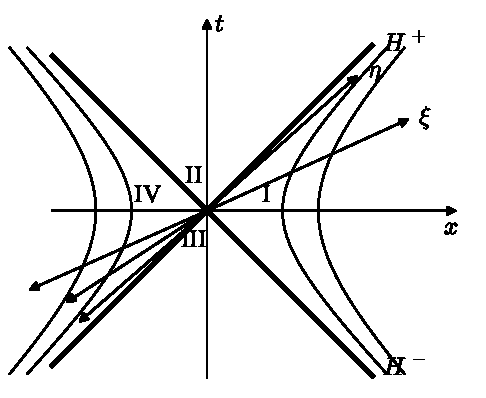
\includegraphics[width=0.72\textwidth]{fig_9.1.pdf}
\caption*{图 9.1\quad Rindler 坐标下的 Minkowski 时空。区域 I 是沿 $+x$ 方向做恒定加速的观者所能到达的区域。坐标 $(\eta,\xi)$ 可用于区域 I，也可单独用于区域 IV，但此时它们指向相反的方向。矢量场 $\partial_{\eta}$ 对应于洛伦兹推动（boost）对称性的生成元。视界 $H^{\pm}$ 是该矢量场的 Killing 视界，同时也是 Rindler 观者所见过去与未来的边界。}
\end{figure}

新坐标的取值范围为

\begin{equation*}
-\infty < \eta,\, \xi < +\infty,
\tag{9.132}
\end{equation*}

并且覆盖楔形区域 $x>|t|$，即图 9.1 中标记为区域 I 的部分。在这些坐标中，恒定加速路径 (9.126) 表为

\begin{align*}
\eta(\tau) &= \frac{\alpha}{a}\tau \\
\xi(\tau) &= \frac{1}{a}\ln\left(\frac{a}{\alpha}\right),
\tag{9.133}
\end{align*}

于是固有时正比于 $\eta$，而空间坐标 $\xi$ 为常数。特别地，$\alpha=a$ 的观者沿如下路径运动：

\begin{equation*}
\eta = \tau, \qquad \xi = 0.
\tag{9.134}
\end{equation*}

在这些坐标中度规取如下形式：

\begin{equation*}
ds^2 = e^{2a\xi}(-d\eta^2 + d\xi^2).
\tag{9.135}
\end{equation*}

带着这个度规，区域 I 被称为\textbf{Rindler 空间}（Rindler space），尽管它显然只是 Minkowski 空间的一部分。\textbf{Rindler 观者}（Rindler observer）就是沿恒定加速路径运动的观者，如 (9.133) 那样。Rindler 空间的因果结构酷似图 5.12 中 Schwarzschild 解最大延拓的 $r>2GM$ 区域。特别地，图 9.1 中标记为 $H^{+}$ 的类光直线 $x=t$，对于区域 I 中任何 $\eta=$ 常数的类空超曲面而言都是未来 Cauchy 视界；类似地，$H^{-}$ 是过去 Cauchy 视界。这些视界让人想起 Kruskal 图中的事件视界：Schwarzschild 中的静态观者（$r=$ 常数）正对应于 Rindler 空间中的恒定加速路径。

(9.135) 中的度规分量与 $\eta$ 无关，所以我们立刻知道 $\partial_{\eta}$ 是一个 Killing 矢量。但当然，这本来就是 Minkowski 时空，所以我们自以为了解所有 Killing 矢量是什么。确实，如果把 $\partial_{\eta}$ 用 $(t,x)$ 坐标表出，我们发现

\begin{align*}
\partial_{\eta} &= \frac{\partial t}{\partial\eta}\partial_t + \frac{\partial x}{\partial\eta}\partial_x \\
&= e^{a\xi}\left[\cosh(a\eta)\partial_t + \sinh(a\eta)\partial_x\right] \\
&= a(x\partial_t + t\partial_x).
\tag{9.136}
\end{align*}

这不多不少，正是与沿 $x$ 方向的推动（boost）相联系的那个 Killing 场。从这个表达式可以清楚地看到，这个 Killing 场自然地延拓到整个时空；在区域 II 和 III 中它是类空的，而在区域 IV 中它是类时的但指向过去。我们上面辨认出的那些视界，实际上就是 $\partial_{\eta}$ 的 Killing 视界。红移因子（在式 (6.12) 中定义为 Killing 矢量范数的大小）为

\begin{equation*}
V = e^{a\xi}.
\tag{9.137}
\end{equation*}

这个 Killing 视界的表面引力 $\kappa=\sqrt{\nabla_{\mu}V\nabla^{\mu}V}$ 于是为

\begin{equation*}
\kappa = a.
\tag{9.138}
\end{equation*}

这里并没有什么真实的引力，因为我们身处平直空间；但这个表面引力刻画了 Rindler 观者的加速度。

我们还可以把 (9.131) 中的符号翻转，在区域 IV 中定义坐标 $(\eta,\xi)$：

\begin{equation*}
t = -\frac{1}{a}e^{a\xi}\sinh(a\eta), \qquad x = -\frac{1}{a}e^{a\xi}\cosh(a\eta) \qquad (x < |t|).
\tag{9.139}
\end{equation*}

这个符号保证了在区域 IV 中 $\partial_{\eta}$ 与 $\partial_t$ 指向相反的方向。严格说来，我们不能在区域 I 和区域 IV 中同时使用 $(\eta,\xi)$，因为这两个坐标在各自区域中的取值范围相同；不过只要我们明确指明所谈论的是哪个区域，就不会出问题。之所以宁愿把同一套坐标标签用两次，而不是干脆引入新坐标，是因为度规 (9.135) 对区域 I 和区域 IV 都适用。

在曲面 $t=0$ 上，$\partial_{\eta}$ 是一个超曲面正交的类时 Killing 矢量，唯一的例外是它为零的那一点 $x=0$。因此这个矢量可用来定义一组正频与负频模式，并在此基础上为标量场的希尔伯特空间搭建 Fock 基。Rindler 坐标下无质量 Klein--Gordon 方程的形式为

\begin{equation*}
\Box\phi = e^{-2a\xi}\left(-\partial_{\eta}^{2} + \partial_{\xi}^{2}\right)\phi = 0.
\tag{9.140}
\end{equation*}

归一化的平面波 $g_k = (4\pi\omega)^{-1/2}e^{-i\omega\eta+ik\xi}$（其中 $\omega=|k|$）求解这个方程，而且显然具有正频，即 $\partial_{\eta}g_k=-i\omega g_k$。但我们需要的模式要相对于一个指向未来的 Killing 矢量具有正频，而在区域 IV 中扮演这一角色的是 $\partial_{(-\eta)}=-\partial_{\eta}$ 而非 $\partial_{\eta}$。为了对付这个麻烦，我们引入两组模式，一组支撑在区域 I 中，另一组支撑在区域 IV 中：

\begin{equation*}
\begin{aligned}
g_{k}^{(1)} &= \begin{cases} \dfrac{1}{\sqrt{4\pi\omega}}\, e^{-i\omega\eta+ik\xi} & \mathrm{I} \\[10pt] 0 & \mathrm{IV} \end{cases} \\[14pt]
g_{k}^{(2)} &= \begin{cases} 0 & \mathrm{I} \\[10pt] \dfrac{1}{\sqrt{4\pi\omega}}\, e^{+i\omega\eta+ik\xi} & \mathrm{IV} \end{cases}
\end{aligned}
\tag{9.141}
\end{equation*}

两种情形下都取 $\omega=|k|$；在两维中，空间波矢就是单独一个数 $k$。每一组模式都相对于相应的指向未来的类时 Killing 矢量具有正频：

\begin{gather*}
\partial_{\eta}\, g_{k}^{(1)} = -i\omega g_{k}^{(1)} \\
\partial_{(-\eta)}\, g_{k}^{(2)} = -i\omega g_{k}^{(2)}, \qquad \omega > 0.
\tag{9.142}
\end{gather*}

这两组模式连同它们的共轭，构成了对整个时空中波动方程任何解都完备的一组基模式。（单独一点 $x=t=0$ 是测度为零的集合，用不着为此担心。）在 Rindler 图的区域 II 和 III 中，这两组模式都不为零；把它们写成坐标 $\eta$ 和 $\xi$ 的形式时这一点被掩盖了，但这些函数可以解析延拓到未来和过去的区域。把相应的湮灭算符记作 $\hat{b}_{k}^{(1,2)}$，我们可以写出

\begin{equation*}
\phi = \int dk\left(\hat{b}_{k}^{(1)}g_{k}^{(1)} + \hat{b}_{k}^{(1)\dagger}g_{k}^{(1)*} + \hat{b}_{k}^{(2)}g_{k}^{(2)} + \hat{b}_{k}^{(2)\dagger}g_{k}^{(2)*}\right).
\tag{9.143}
\end{equation*}

这一展开是 (9.66) 式——用原始 Minkowski 模式所作的展开——的另一种选择；在两维中该式取如下形式：

\begin{equation*}
\phi = \int dk\left(\hat{a}_{k}f_{k} + \hat{a}_{k}^{\dagger}f_{k}^{*}\right).
\tag{9.144}
\end{equation*}

容易直接检验，模式 (9.141) 相对于内积 (9.94) 是恰当归一化的。在度规 (9.135) 中，曲面 $\eta=0$ 的指向未来的单位法矢量归一化为

\begin{equation*}
-1 = g_{\mu\nu}n^{\mu}n^{\nu} = -e^{2a\xi}(n^{0})^{2},
\tag{9.145}
\end{equation*}

即

\begin{equation*}
n^{0} = e^{-a\xi}.
\tag{9.146}
\end{equation*}

与此同时，空间度规的行列式满足

\begin{equation*}
\sqrt{\gamma} = e^{a\xi}.
\tag{9.147}
\end{equation*}

于是我们有 $n^{0}\sqrt{\gamma}=1$，而 Rindler 模式内积的计算与普通 Minkowski 模式的计算如出一辙。最终得到

\begin{align*}
(g_{k_1}^{(1)}, g_{k_2}^{(1)}) &= \delta(k_1 - k_2) \\
(g_{k_1}^{(2)}, g_{k_2}^{(2)}) &= \delta(k_1 - k_2) \\
(g_{k_1}^{(1)}, g_{k_2}^{(2)}) &= 0,
\tag{9.148}
\end{align*}

共轭模式也有类似结果。

这样就有两组模式——Minkowski 模式与 Rindler 模式——都可以用来展开平直两维时空中 Klein--Gordon 方程的解。虽然理论的希尔伯特空间在两种表示下是同一个，但它作为 Fock 空间的诠释却会不同；特别地，真空态会不相同。Minkowski 真空 $|0_{\mathrm{M}}\rangle$ 满足

\begin{equation*}
\hat{a}_{k}|0_{\mathrm{M}}\rangle = 0,
\tag{9.149}
\end{equation*}

在 Rindler 表示中它将被描述为一个多粒子态；同样，Rindler 真空 $|0_{\mathrm{R}}\rangle$ 满足

\begin{equation*}
\hat{b}_{k}^{(1)}|0_{\mathrm{R}}\rangle = \hat{b}_{k}^{(2)}|0_{\mathrm{R}}\rangle = 0,
\tag{9.150}
\end{equation*}

在 Minkowski 表示中它将被描述为一个多粒子态。在实际层面上，这种差异源于：单个 Rindler 模式永远无法写成正频 Minkowski 模式之和；在 $t=0$ 处 Rindler 模式只有支撑在半直线上的部分，而这样的函数不可能展开成纯粹正频的平面波。因此，用来定义 $|0_{\mathrm{R}}\rangle$ 的那些 Rindler 湮灭算符必然是 Minkowski 产生算符与湮灭算符的叠加，所以两个真空不可能重合。

Rindler 观者相对于推动 Killing 矢量 $\partial_{\eta}$ 的轨道是静止的。因此区域 I 中的这种观者将用 Rindler 模式 $g_{k}^{(1)}$ 来描述粒子：特别地，他会观测到 Rindler 真空中的态不含粒子，态 $\hat{b}_{k}^{(1)\dagger}|0_{\mathrm{R}}\rangle$ 含有一个频率为 $\omega=|k|$ 的粒子，如此等等。反过来，一位穿过 Minkowski 真空态的 Rindler 观者将探测到一个粒子背景，尽管惯性观者会把这个态描述成完全空无一物。Rindler 观者会探测到什么样的粒子呢？我们知道怎样回答这个问题：计算联系 Minkowski 模式与 Rindler 模式的 Bogoliubov 系数，再用它们确定 Rindler 粒子数算符在 Minkowski 真空中的期望值。这直截了当却十分繁琐，所以我们将走一条由 Unruh 提出的捷径。我们将找到一组模式，它与 Minkowski 模式共享同一个真空态（尽管对激发态的描述可能不同），但它与 Rindler 模式的交叠更为直接。做法是：从 Rindler 模式出发，把它们解析延拓到整个时空，再把这一延拓用原始的 Rindler 模式表出。

为了看清这是如何运作的，注意由 (9.131) 和 (9.139) 可知，在区域 I 和 IV 中，Minkowski 坐标 $(t,x)$ 与 Rindler 坐标 $(\eta,\xi)$ 之间有如下关系：

\begin{equation*}
\begin{aligned}
e^{-a(\eta-\xi)} &= \begin{cases} a(-t+x) & \mathrm{I} \\ a(t-x) & \mathrm{IV} \end{cases} \\[10pt]
e^{a(\eta+\xi)} &= \begin{cases} a(t+x) & \mathrm{I} \\ a(-t-x) & \mathrm{IV} \end{cases}
\end{aligned}
\tag{9.151}
\end{equation*}

因此，对于 $k>0$（从而 $\omega=k$）的模式 $g_{k}^{(1)}$，其在区域 I 中用 Minkowski 坐标表出的时空依赖为

\begin{align*}
\sqrt{4\pi\omega}\, g_{k}^{(1)} &= e^{-i\omega\eta+ik\xi} \\
&= e^{-i\omega(\eta-\xi)} \\
&= a^{i\omega/a}(-t+x)^{i\omega/a}.
\tag{9.152}
\end{align*}

这个函数在整个时空中的解析延拓很直截了当：对任何 $(t,x)$ 值都用这最后一个表达式即可。但我们希望处处都用原始的 Rindler 模式来表示结果；由于 $g_{k}^{(1)}$ 模式在区域 IV 中为零，我们需要让 $g_{k}^{(2)}$ 模式登场。在区域 IV 中用 Minkowski 坐标表出这些模式，对 $k>0$ 得到

\begin{align*}
\sqrt{4\pi\omega}\, g_{k}^{(2)} &= e^{+i\omega\eta+ik\xi} \\
&= e^{+i\omega(\eta+\xi)} \\
&= a^{-i\omega/a}(-t-x)^{-i\omega/a}.
\tag{9.153}
\end{align*}

这与我们想要的 (9.152) 的行为并不匹配。但若取复共轭并反转波数，就得到

\begin{align*}
\sqrt{4\pi\omega}\, g_{-k}^{(2)*} &= e^{-i\omega\eta+ik\xi} \\
&= e^{-i\omega(\eta-\xi)} \\
&= a^{i\omega/a}(t-x)^{i\omega/a} \\
&= a^{i\omega/a}[e^{-i\pi}(-t+x)]^{i\omega/a} \\
&= a^{i\omega/a}e^{\pi\omega/a}(-t+x)^{i\omega/a}.
\tag{9.154}
\end{align*}

组合

\begin{equation*}
\sqrt{4\pi\omega}\left(g_{k}^{(1)} + e^{-\pi\omega/a}g_{-k}^{(2)*}\right) = a^{i\omega/a}(-t+x)^{i\omega/a}
\tag{9.155}
\end{equation*}

因此沿整个曲面 $t=0$ 都有良好定义。我们明确考察了 $k>0$ 的情形，但对 $k<0$ 会得到完全相同的结果。

这个模式的恰当归一化版本由下式给出：

\begin{equation*}
h_{k}^{(1)} = \frac{1}{\sqrt{2\sinh\left(\frac{\pi\omega}{a}\right)}}\left(e^{\pi\omega/2a}g_{k}^{(1)} + e^{-\pi\omega/2a}g_{-k}^{(2)*}\right).
\tag{9.156}
\end{equation*}

这是 $g_{k}^{(1)}$ 模式的一个恰当的解析延拓；为了得到完备集，还需纳入 $g_{k}^{(2)}$ 模式的延拓，由类似的论证可知它为

\begin{equation*}
h_{k}^{(2)} = \frac{1}{\sqrt{2\sinh\left(\frac{\pi\omega}{a}\right)}}\left(e^{\pi\omega/2a}g_{k}^{(2)} + e^{-\pi\omega/2a}g_{-k}^{(1)*}\right).
\tag{9.157}
\end{equation*}

为了验证归一化——比如对 $h_{k}^{(1)}$——我们利用 (9.148)：

\begin{align*}
\left(h_{k_1}^{(1)}, h_{k_2}^{(1)}\right) &= \frac{1}{2\sqrt{\sinh\left(\frac{\pi\omega_1}{a}\right)\sinh\left(\frac{\pi\omega_2}{a}\right)}}\Bigg[e^{\pi(\omega_1+\omega_2)/2a}\left(g_{k_1}^{(1)}, g_{k_2}^{(1)}\right) \\
&\quad + e^{-\pi(\omega_1+\omega_2)/2a}\left(g_{-k_1}^{(2)*}, g_{-k_2}^{(2)*}\right)\Bigg] \\
&= \frac{1}{2\sqrt{\sinh\left(\frac{\pi\omega_1}{a}\right)\sinh\left(\frac{\pi\omega_2}{a}\right)}}\Bigg[e^{\pi(\omega_1+\omega_2)/2a}\,\delta(k_1 - k_2) \\
&\quad + e^{-\pi(\omega_1+\omega_2)/2a}\,\delta(-k_1 + k_2)\Bigg] \\
&= \frac{e^{\pi\omega_1/a} - e^{-\pi\omega_1/a}}{2\sinh\left(\frac{\pi\omega_1}{a}\right)}\,\delta(k_1 - k_2) \\
&= \delta(k_1 - k_2),
\tag{9.158}
\end{align*}

正如我们所愿。

现在可以把场用这些模式展开：

\begin{equation*}
\phi = \int dk\left(\hat{c}_{k}^{(1)}h_{k}^{(1)} + \hat{c}_{k}^{(1)\dagger}h_{k}^{(1)*} + \hat{c}_{k}^{(2)}h_{k}^{(2)} + \hat{c}_{k}^{(2)\dagger}h_{k}^{(2)*}\right).
\tag{9.159}
\end{equation*}

根据 9.4 节中关于 Bogoliubov 变换的讨论我们知道，用 $g_{k}^{(1,2)}$ 模式表出 $h_{k}^{(1,2)}$ 模式的表达式 (9.156) 与 (9.157)，蕴含着用算符 $\hat{c}_{k}^{(1,2)}$ 表出 Rindler 算符 $\hat{b}_{k}^{(1,2)}$ 的相应表达式：

\begin{align*}
\hat{b}_{k}^{(1)} &= \frac{1}{\sqrt{2\sinh\left(\frac{\pi\omega}{a}\right)}}\left(e^{\pi\omega/2a}\hat{c}_{k}^{(1)} + e^{-\pi\omega/2a}\hat{c}_{-k}^{(2)\dagger}\right) \\
\hat{b}_{k}^{(2)} &= \frac{1}{\sqrt{2\sinh\left(\frac{\pi\omega}{a}\right)}}\left(e^{\pi\omega/2a}\hat{c}_{k}^{(2)} + e^{-\pi\omega/2a}\hat{c}_{-k}^{(1)\dagger}\right).
\tag{9.160}
\end{align*}

于是我们可以把区域 I 中的 Rindler 粒子数算符

\begin{equation*}
\hat{n}_{\mathrm{R}}^{(1)}(k) = \hat{b}_{k}^{(1)\dagger}\hat{b}_{k}^{(1)},
\tag{9.161}
\end{equation*}

用新的算符 $\hat{c}_{k}^{(1,2)}$ 表示。

原先 $k>0$ 的正频 Minkowski 平面波模式 $f_k\propto e^{-i\omega(t-x)}$，只要 $\mathrm{Im}(t-x)\leq 0$，对复的 $(t,x)$ 都是解析且有界的。（这类模式称为“右行”（right-moving），因为它们描述向右传播的波。）只要我们把虚幂函数的支割线取在上半复 $(t-x)$ 平面内，我们的新模式 $h_{k}^{(1)}$ 也具有同样的性质——考察 (9.152) 和 (9.154) 即可看出；这与我们在 (9.154) 中取 $-1=e^{-i\pi}$ 的做法是一致的。类似的考虑也适用于 $h_{k}^{(2)}$ 模式，它们在下半复 $(t+x)$ 平面内解析且有界，正如 $k<0$ 的正频 Minkowski 平面波模式（左行）一样。因此，与原先的 Rindler 模式 $g_{k}^{(1,2)}$ 不同，我们知道 $h_{k}^{(1,2)}$ 模式能够纯粹用正频 Minkowski 模式 $f_k$ 表出。所以它们与 Minkowski 模式共享同一个真空态 $|0_{\mathrm{M}}\rangle$，于是

\begin{equation*}
\hat{c}_{k}^{(1)}|0_{\mathrm{M}}\rangle = \hat{c}_{k}^{(2)}|0_{\mathrm{M}}\rangle = 0.
\tag{9.162}
\end{equation*}

激发态将不会重合，但这不会困扰我们，因为我们关心的正是当态恰好处于 Minkowski 真空时 Rindler 观者会看到什么。例如，区域 I 中的观者将观测由算符 $\hat{b}_{k}^{(1)}$ 定义的粒子；频率为 $\omega$ 的这类粒子的期望数目由下式给出：

\begin{align*}
\langle 0_{\mathrm{M}}|\hat{n}_{\mathrm{R}}^{(1)}(k)|0_{\mathrm{M}}\rangle &= \langle 0_{\mathrm{M}}|\hat{b}_{k}^{(1)\dagger}\hat{b}_{k}^{(1)}|0_{\mathrm{M}}\rangle \\
&= \frac{1}{2\sinh\left(\frac{\pi\omega}{a}\right)}\langle 0_{\mathrm{M}}|e^{-\pi\omega/a}\hat{c}_{-k}^{(1)}\hat{c}_{-k}^{(1)\dagger}|0_{\mathrm{M}}\rangle \\
&= \frac{e^{-\pi\omega/a}}{2\sinh\left(\frac{\pi\omega}{a}\right)}\,\delta(0) \\
&= \frac{1}{e^{2\pi\omega/a} - 1}\,\delta(0),
\tag{9.163}
\end{align*}

其中我们用到了 $\hat{c}_{k}^{(1)\dagger}|0_{\mathrm{M}}\rangle$ 是归一化的单粒子态这一事实：

\begin{equation*}
\langle 0_{\mathrm{M}}|\hat{c}_{k}^{(1)}\hat{c}_{k}^{(1)\dagger}|0_{\mathrm{M}}\rangle = \delta(0).
\tag{9.164}
\end{equation*}

(9.163) 中的 $\delta$ 函数只是我们使用（不可平方可积的）平面波基模式带来的假象；如果我们构造的是归一化的波包，就会得到一个有限的结果，而谱完全相同。

结果 (9.163) 是一个温度为

\begin{equation*}
T = \frac{a}{2\pi}.
\tag{9.165}
\end{equation*}

的 Planck 谱。这样，\emph{以均匀加速度穿过 Minkowski 真空运动的观者会观测到粒子的热谱}。这就是\textbf{安鲁效应}。当然，热辐射不只是谱 (9.163) 而已；要真正称得上热，我们还应当检查在观测到的粒子之间没有隐匿的关联。这一点已经得到验证：Rindler 观者探测到的辐射是真正热的。在最基本的层面上，安鲁效应表明两批不同的观者（惯性的与 Rindler 的）会用极为不同的语言描述同一个态；在稍稍深入的层面上，它揭示了量子场论中真空本质上的热性质。

温度 $T=a/2\pi$ 是沿路径 $\xi=0$ 运动的观者会测得的温度，这条路径感受到的加速度为 $\alpha=a$。利用 (9.133) 可知，任何 $\xi=$ 常数的其他路径感受到的加速度为

\begin{equation*}
\alpha = ae^{-a\xi}
\tag{9.166}
\end{equation*}

因而应当测得温度为 $\alpha/2\pi$ 的热辐射。这与我们在第 6 章中关于沿某个 Killing 矢量 $K^{\mu}$ 的轨道运动的静态观者所见证的红移的讨论相一致；我们当时发现，在点 $x_1$ 处以频率 $\omega_1$ 发出的辐射，将在点 $x_2$ 处被观测到具有频率

\begin{equation*}
\omega_2 = \frac{V_1}{V_2}\omega_1,
\tag{9.167}
\end{equation*}

其中红移因子 $V$ 是 Killing 矢量的范数。在 (9.137) 中我们发现与 $\partial_{\eta}$ 相联系的红移因子为 $V=e^{a\xi}$，于是

\begin{equation*}
\omega_2 = e^{a(\xi_1 - \xi_2)}\omega_1.
\tag{9.168}
\end{equation*}

因此，如果 $\xi_1=0$ 处的观者探测到温度 $T=a/2\pi$，那么 $\xi_2=\xi$ 处的观者将看到它红移为温度 $T=ae^{-a\xi}/2\pi$，正如式 (9.166) 那样。特别地，当 $\xi\to+\infty$ 时温度一路红移到零。这是有道理的：无穷远处的 Rindler 观者近乎惯性观者，会对真空和粒子给出与普通 Minkowski 观者相同的定义。

安鲁效应告诉我们，加速观者会在 Minkowski 真空态中探测到粒子。当然，惯性观者会把同一个态描述成完全空无一物；实际上，能动张量的期望值会是 $\langle T_{\mu\nu}\rangle=0$。可是如果没有能量-动量，Rindler 观者们怎么能探测到粒子呢？这是一个微妙的问题，但绝不是矛盾。Rindler 观者要探测背景粒子，就必须携带一台探测器——某种与被探测粒子相耦合的装置。但如果探测器被维持在恒定加速度下，能量就不守恒；我们需要持续对探测器做功才能让它一直加速。从 Minkowski 观者的角度看，Rindler 探测器\emph{发射}粒子，也同样吸收粒子；一旦引入耦合，发射的可能性就不可避免。当探测器记录到一个粒子时，惯性观者会说它发射了一个粒子，并因此感受到一个辐射反作用力。归根结底，激发 Rindler 探测器所需的能量并非来自背景能动张量，而是来自我们为维持探测器加速而注入的能量。

\section{霍金效应与黑洞蒸发}

尽管发生在平直时空，安鲁效应却给了我们弯曲时空量子场论最重要的一课：“真空”和“粒子”是依赖于观者的概念，而非基本概念。实际上，鉴于我们对安鲁效应的理解，几乎可以立刻看出霍金效应是如何产生的。这不应太令人惊讶，因为我们已经指出过 Rindler 空间的因果结构与描述永恒黑洞的最大延拓 Schwarzschild 时空的因果结构之间的相似性。因此，我们将能够论证霍金辐射的存在，而无需在弯曲时空中做任何显式计算；当然，还有许多你可能想更深入考察的特征，那就需要充分动用弯曲度规的力量。除 Birrell 和 Davies (1982) 与 Wald (1994) 之外，还有一些很好的综述文章，你可以在其中找到对这里讨论的问题更全面的讨论。\footnote{T.A. Jacobson, “Introductory Lectures on Black Hole Thermodynamics,” Lectures at University of Utrecht (1996), http://www.fys.ruu.nl/\textasciitilde{}wwwthe/lectures/itfuu-0196.ps; R.M. Wald, “The thermodynamics of black holes,” \emph{Living Rev.\ Rel.} \textbf{4}, 6 (2001), http://arxiv.org/gr-qc/9912119; J. Traschen, “An introduction to black hole evaporation” (2000), http://arxiv.org/gr-qc/0010055.} 我们对霍金辐射的推导沿循 Jacobson 的做法。

考虑一个位于 Schwarzschild 黑洞之外、半径 $r_{1} > 2GM$ 处的静态观者。这样的观者沿着类时 Killing 矢量 $K = \partial_{t}$ 的轨道运动。在第 6 章中我们已经证明，对 Schwarzschild 时空中的静态观者，红移因子 $V = \sqrt{-K_{\mu}K^{\mu}}$ 由下式给出

\begin{equation*}
V = \sqrt{1 - \frac{2GM}{r}},
\tag{9.169}
\end{equation*}

相应的加速度大小则由下式给出：

\begin{equation*}
a = \frac{GM}{r\sqrt{r - 2GM}}.
\tag{9.170}
\end{equation*}

对于非常靠近事件视界的观者，$r_{1} - 2GM \ll 2GM$，这一加速度与 Schwarzschild 半径所标定的尺度相比会变得非常大，

\begin{equation*}
a_{1} \gg \frac{1}{2GM}.
\tag{9.171}
\end{equation*}

Schwarzschild 半径又标定了视界附近时空的曲率半径。因此，在由 $a_{1}^{-1} \ll 2GM$ 所设定的长度和时间尺度上观察，时空看上去基本上是平直的。让我们作一个至关重要的假设：在黑洞附近\emph{自由下落}的观者看来，某个标量场 $\phi$ 的量子态就像 Minkowski 真空（不含任何粒子）。这个假设是合理的，因为事件视界并不是一种局域的屏障；自由下落的观者在穿过视界时看不到任何异常发生。于是，这位静态观者看起来就跟平直时空中的常加速度观者一模一样，将探测到温度为 $T_{1} = a_{1}/2\pi$ 的安鲁辐射。

现在考虑位于无限远处——或者至少位于与 $2GM$ 相比大得多的距离 $r_{2}$ 处——的静态观者。在这种情形下，无论如何都谈不上能在 $a_{2}^{-1} \gg 2GM$ 的时间尺度上忽略时空曲率，因此没有理由预期他们会看到温度为 $a_{2}/2\pi$ 的辐射，这里 $a_{2}$ 在 $r_{2}$ 处取值。但是在视界附近观测到的辐射会带着恰当的红移传播到无限远。我们可以套用上一节末尾用过的论证，来确定这样的观者应当会看到什么；他们应当探测到红移至如下温度的热辐射：

\begin{equation*}
T_{2} = \frac{V_{1}}{V_{2}} T_{1} = \frac{V_{1}}{V_{2}} \frac{a}{2\pi}.
\tag{9.172}
\end{equation*}

在无限远处 $V_{2} \to 1$，于是观测到的温度为

\begin{equation*}
T = \lim_{r_{1} \to 2GM} \frac{V_{1} a_{1}}{2\pi} = \frac{\kappa}{2\pi},
\tag{9.173}
\end{equation*}

其中 $\kappa = \lim(Va)$ 是表面引力；对 Schwarzschild 黑洞，$\kappa = 1/4GM$。与平直时空中的加速观者不同，Schwarzschild 时空中的静态 Killing 矢量在无限远处具有有限的模长，因此视界附近的辐射只红移到一个有限值，而不会一直红移到零。远离黑洞的观者因此会看到黑洞发出的热辐射流，其温度正比于黑洞的表面引力。这就是著名的\textbf{霍金效应}（Hawking effect），这种辐射本身则被称为霍金辐射。

这种对霍金效应的推导虽然取巧，却没有任何不诚实之处。特别是，与加速度的联系清楚地说明了为什么温度正比于黑洞的表面引力（这一结论对更一般的黑洞同样成立，而不只是 Schwarzschild 黑洞）。不过，我们需要对我们所作的那个假设有清醒的认识：视界附近的真空态在自由下落的观者看来是非奇异的。用术语来说，就是取重整化能动张量在视界处为有限，或者等价地，两点函数满足 Hadamard 条件 (9.123)。

通过考察最大延拓 Schwarzschild 几何中各种可能的真空态，这个假设的含义会变得更加清楚。这些态对于由引力坍缩形成的现实黑洞来说不一定具有物理上的相关性，但在这种理想化情形中出现的各种可能性，能给现实世界带来有益的教益。我们将只描述这些态，而不定量地刻画它们，也不推导它们的任何性质；更多细节可参见上文所引的文献。

在寻找真空态时，我们也许会先去寻找一个在整个时空中都正则的态［在 Hadamard 意义下，式 (9.123)］。对最大延拓的 Schwarzschild 时空，Hartle 和 Hawking 找到了这样一个态，我们称之为\textbf{Hartle--Hawking 真空}（Hartle--Hawking vacuum）；的确，这是唯一的既处处正则、又在代表无限远处时间平移的 Schwarzschild Killing 矢量 $\partial_{t}$ 作用下不变的真空态。特别是，回忆图 5.16 所示的 Schwarzschild 共形图，Hartle--Hawking 真空在 $r = 2GM$ 处的过去和未来事件视界 $H^{\pm}$ 上正则，在过去和未来类光无限远 $\mathscr{I}^{\pm}$ 上也正则。根据上文对静态观者的讨论，我们应当会预期 Hartle--Hawking 真空中有热辐射从黑洞发出，而事实证明确实如此。然而，对这个态的仔细考察揭示出，还有一份等量的热辐射流从过去类光无限远（$\mathscr{I}^{-}$）流向黑洞；换句话说，它描述的是一个与其环境处于热平衡的黑洞。我们并不会用它来模拟我们宇宙中现实的黑洞。另一种真空更类似于经由引力坍缩形成的黑洞的真空态，这就是\textbf{Unruh 真空}（Unruh vacuum），它在 $H^{+}$ 上非奇异（因此预言了出射的霍金辐射），但没有来自 $\mathscr{I}^{-}$ 的入射辐射。Unruh 真空在 Schwarzschild 的过去视界 $H^{-}$ 上是奇异的；如果我们只是把它当作现实黑洞的模型，这并不会困扰我们，因为如图 5.17 那样经历引力坍缩的时空不会有白洞，也没有任何过去视界。最后，我们也许会去寻找这样一种真空态：既没有粒子进入黑洞，也没有粒子逃往无限远；换句话说，$\mathscr{I}^{\pm}$ 上通量为零。确实存在这样一个态，称为\textbf{Boulware 真空}（Boulware vacuum）。这样一种态的存在，似乎与我们从安鲁效应出发对霍金效应所作的论证相冲突，但仔细的分析表明，Boulware 真空在 $H^{-}$ 和 $H^{+}$ 上都是奇异的。于是，认为真空在视界附近的自由下落观者看来是正则的这一假设，在这个态中被违反了。

因此，对永恒 Schwarzschild 度规中真空态的仔细考察，与我们基于安鲁效应的推理是一致的；在 $H^{+}$ 上正则的态预言了预期形式的霍金辐射。注意，事件视界的存在对这一论证至关重要；如果没有这样的视界，态必须在视界上正则的要求就没有任何约束力。以中子星为例：其半径可能接近 Schwarzschild 半径，但其时空没有任何视界。中子星不发出任何霍金辐射。理解这一点的一个途径是认识到，静态中子星度规具有一个处处类时的 Killing 矢量，可以用它来定义贯穿整个时空延伸、并且在无限远处与 Minkowski 模式相匹配的正频模式。这样得到的真空态实际上会类似于 Boulware 真空，在 $\mathscr{I}^{\pm}$ 上没有通量；而完整的 Boulware 真空在视界上奇异这一点，在中子星情形中不会困扰我们，因为那里根本不存在任何视界。

为了绝对确信我们为现实的黑洞正确选择了真空态，我们应当考虑在一个过去近乎 Minkowski 时空、未来为 Schwarzschild 时空的时空中发生的引力坍缩，如图 5.17 所示。如果真空在 $\mathscr{I}^{-}$ 上取标准的 Minkowski 形式，我们就可以追问这些模式如何穿过坍缩几何传播到 $\mathscr{I}^{+}$，这就定义了一个如式 (9.45) 中的 S 矩阵，用以确定渐近观者会看到什么。Hawking 最初发现黑洞辐射时所做的正是这件事；计算涉及一些烦琐的代数，但基本上是直截了当的，得到的温度与我们上面推导的相同。

当然，从完整的计算中我们能学到的不仅仅是黑体温度；我们会想问，比如说，当发射辐射的波长与 Schwarzschild 半径相当时会发生什么——在这种情形下我们的近似显然失效了。如果我们仔细研究任意种类的粒子从任何一种黑洞（也就是同时容许电荷和自旋）的发射，就会发现发射辐射的谱具有如下形式

\begin{equation*}
\langle \hat{n}_{\omega} \rangle = \frac{\Gamma(\omega)}{e^{2\pi(\omega - \mu)/\kappa} \pm 1}.
\tag{9.174}
\end{equation*}

这里的 $\kappa$ 当然就是表面引力。参数 $\mu$ 是一个化学势（chemical potential），刻画黑洞丢掉其守恒量子数的倾向；带电黑洞优先发射与黑洞电荷同号的粒子，而转动黑洞优先发射与黑洞角动量同号的粒子。因此，霍金辐射趋向于把黑洞带回 Schwarzschild 状态。$\Gamma(\omega)$ 是一个灰体因子（greybody factor），可以把它想象成波包被引力场反散射回黑洞而产生的。在高频极限下波长非常小，反散射可以忽略；在极低的频率下，波长变得大于 Schwarzschild 半径，反散射就变得重要起来。虽然灰体因子的解析表达式很难导出，但在频率很大和很小的极限情形下，标量场的灰体因子满足

\begin{align*}
\Gamma(\omega) &\to 1, \qquad \omega \gg \frac{1}{GM} \\
\Gamma(\omega) &\to \frac{A}{4\pi} \omega^{2}, \qquad \omega \ll \frac{1}{GM},
\tag{9.175}
\end{align*}

其中 $A$ 是黑洞的面积。

从经典广义相对论的观点来看，黑洞发出热辐射的发现当然是令人惊讶的，因为我们曾经强调过，从事件视界内部的点逃逸到无限远是不可能的。理解眼下情形的一种形象方式，是用 Feynman 图来思考真空涨落：涨落由不断地出现又消失的虚粒子/反粒子对来表示。这幅图像也很有帮助，例如有助于理解诸如 Lamb 位移（Lamb shift）这样的观测现象——原子光谱会受到光子与虚电子/正电子对相互作用的影响。通常情况下，这些粒子对总会湮灭，它们的效应只是间接的，通过与虚粒子相耦合的过程的重整化体现出来。然而，在存在事件视界时，虚粒子对中的一个成员偶尔会落入黑洞，而它的同伴则逃逸到无限远，如图 9.2 所描绘。在这幅图像中，我们观测为霍金辐射的正是这些逃逸的虚粒子。虚粒子对的总能量必须相加为零，但从无限远来看，落入的粒子可以带有负能量，因为渐近类时的 Killing 矢量在视界内部是类空的。这幅图像有些不正规，但它为正在发生的事情提供了一种有用的启发。

\begin{figure}[H]
\centering
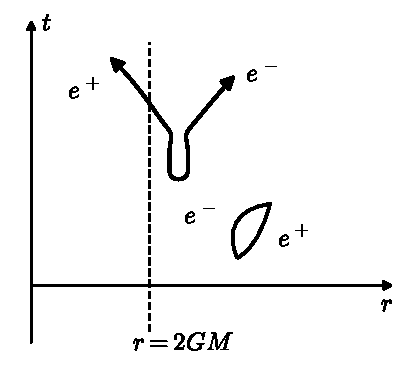
\includegraphics[width=0.72\textwidth]{fig_9.2.pdf}
\caption*{图 9.2\quad 真空涨落偶尔会导致粒子/反粒子对中的一个落入事件视界，而另一个则作为霍金辐射逃逸到无限远。}
\end{figure}

一旦知道了黑洞温度的公式，我们就能够确定黑洞参数与热力学变量之间各关系式中的比例常数，如式 (6.118) 所列。霍金辐射可以说最终圆满成就了黑洞力学与热力学的联姻；稳态黑洞的行为就如同能量 $E = M$、温度 $T = \kappa/2\pi$、熵 $S = A/4G$ 的热平衡物体。这确实是极其巨大的熵。对宇宙中的物质场而言，熵近似等于相对论性粒子的数目；在一个 Hubble 半径之内，这个数目算出来是

\begin{equation*}
S_{\mathrm{M}} \sim 10^{88}.
\tag{9.176}
\end{equation*}

另一方面，黑洞的熵是以 Planck 单位量度的视界面积（记住，我们从头到尾都在取 $\hbar = 1$）。我们可以换算成天体物理单位，得到

\begin{equation*}
S_{\mathrm{BH}} \sim 10^{90} \left( \frac{M}{10^{6} M_{\odot}} \right)^{2}.
\tag{9.177}
\end{equation*}

这样，单个百万太阳质量的黑洞（例如在我们自己银河系的中心以及许多其他星系的中心就能找到）所具有的熵，就比可见宇宙中全部物质的熵还要多。宇宙的总熵远比我们本来能把它做到的要小——只要把更多的质量投入黑洞就行。（当宇宙学家说熵 $S_{\mathrm{M}}$ 很大时，他们的意思是：在一个曲率半径之内竟然存在这么多熵，这很令人惊讶。）我们之所以处在这样一个低熵状态，其原因想必与初始条件有关，或许还与暴胀有关。

回到黑洞力学，我们看到一个难题：宏观黑洞的熵会非常巨大，但从统计力学的观点来看，熵本应量度可及态数目的对数。经典黑洞由少数几个参数（质量、电荷和自旋）确定，因此很难知道那些态可能是什么。尽管如此，我们可以采取这样的态度：这个矛盾其实无关紧要，因为关于黑洞状态的任何信息想必都藏在事件视界背后。

把量子力学包括进来，使这个难题变得更糟而非更好，因为黑洞不仅会辐射，而且会蒸发。当我们开始研究弯曲时空中的 QFT 时，我们定下的规则之一就是：假定背景度规固定不变，不去操心量子场自身的能动张量会产生什么影响。尽管如此，即使在量子力学中我们也有能量守恒（例如，表现为渐近平直时空中守恒的 ADM 质量）。因此，当霍金辐射逃逸到无限远时，我们可以放心地断定，它会把能量从黑洞带走，黑洞的质量必然因此缩减。（这个现象并不违反面积定理，因为量子场的能动张量在视界附近将不满足弱能量条件。）随着质量缩减，表面引力增大，温度也随之升高；这是一个失控的过程，全部质量会在有限的时间内蒸发殆尽。代入数值，可以得到量级如下的寿命

\begin{equation*}
\tau_{\mathrm{BH}} \sim \left( \frac{M}{m_{\mathrm{P}}} \right)^{3} t_{\mathrm{P}} \sim \left( \frac{M}{M_{\odot}} \right)^{3} \times 10^{71}\,\mathrm{sec},
\tag{9.178}
\end{equation*}

其中 $m_{\mathrm{P}} \sim 10^{-5}\,\mathrm{g}$ 是 Planck 质量，$t_{\mathrm{P}} \sim 10^{-43}\,\mathrm{sec}$ 是 Planck 时间。由于 Hubble 时间为 $H_{0}^{-1} \sim 10^{18}\,\mathrm{sec}$，一个太阳质量黑洞的寿命约为宇宙年龄的 $10^{53}$ 倍。这看起来是很长的时间，但我们在这里谈论的是原理性的问题。

你可以看出为什么黑洞熵的问题变得如此严峻：一旦黑洞蒸发殆尽，我们就不能再求助于事件视界来隐藏黑洞那些所谓的态。黑洞不复存在，只剩下它产生的霍金辐射。这种辐射被认为应当是严格热性的（出射粒子中没有隐藏的关联），这一事实意味着，它没有任何办法传递巨量的信息，而指定我们的熵计算所隐含的那些态正需要这些信息。这样一来，如果我们把两个非常不同的初始态分别坍缩成两个质量、电荷和自旋都相同的黑洞，它们就会辐射成两团不可分辨的霍金粒子云。系统在变成黑洞之前、为规定其状态而投入的信息，看来已被抹去；这就是\textbf{信息丢失佯谬}（information loss paradox）。量子场论和广义相对论都以幺正演化为特征——指定早期时刻的一个态所需的信息，与指定较晚时刻的一个态所需的信息严格相等，因为二者通过运动方程联系在一起。但在把 QFT 与 GR 结合的过程中，这种幺正性显然被破坏了。看来很可能我们在论证的某个地方作了某个不恰当的假设，但很难看出在哪里。

传达信息丢失佯谬实质的一个途径，是考察图 9.3 所示的设想中的蒸发黑洞共形图。我们并不真正知道完整的时空应当是什么样子，但这里我们作了似乎合理的假设：形成一个奇点，以及一个与之相伴随的事件视界，二者在黑洞完全蒸发后都消失，留下一个具有 Minkowski 型因果结构的时空。如果我们用 Cauchy 面来思考，问题就显而易见了。一张从类空无限远 $i^{0}$ 延伸到奇点过去侧某个 $r = 0$ 点的非编时面，其未来依赖域将是整个时空，因此这样的面会是一个 Cauchy 面。但是一张延伸到奇点未来侧某个 $r = 0$ 点的类似的面就不是 Cauchy 面了，因为事件视界背后的区域不在它的依赖域之中。因此，由于信息消失于奇点，过去无法由未来反推。换句话说，这个过程看起来是时间不可逆的（在微观意义上，而不仅仅是统计意义上），尽管用来预言它的动力学定律在时间反演下是完全不变的。

\begin{figure}[H]
\centering
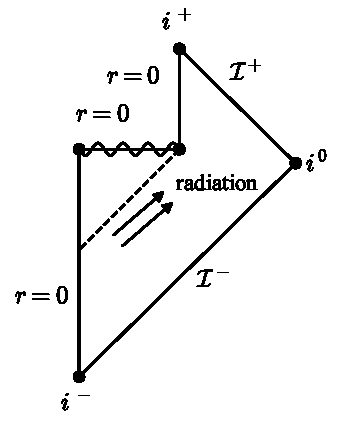
\includegraphics[width=0.72\textwidth]{fig_9.3.pdf}
\caption*{图 9.3\quad 设想中的蒸发黑洞共形图。能量被霍金辐射带走，黑洞最终完全蒸发殆尽，留下具有 Minkowski 时空因果结构的未来。落过事件视界进入奇点的信息看起来丢失了。}
\end{figure}

在讨论信息丢失佯谬时，请记住我们对黑洞蒸发的分析只是在量子场论与广义相对论相耦合的混合理论中进行的，并不是在现实的量子引力理论中。真实世界里究竟可能发生着什么呢？一种可能性是信息真的会丢失，幺正性真的会被破坏，而我们只得学会与之共处。许多物理学家觉得，引入这样一种可预见性的根本失效令人难以接受，而且也有论证表明，幺正性的破坏必然会导致能量守恒的破坏。另一种可能性是，幺正性在我们的世界中看似被破坏，只是因为进入黑洞的信息以某种方式逃逸到了空间一个不相连通的区域——一个婴儿宇宙（baby universe）。广义相对论预言黑洞中心存在奇点，而不是产生一个不相连通的区域；但显然我们正处于量子效应将剧烈改变经典预期的领域，所以我们应当保持开放的心态。

反对信息丢失的一些证据来自弦论。弦论自然地在 10 或 11 维时空中定义，其特征不仅在于一维的延展客体（弦），还在于统称为“膜”（branes）的各种更高维的延展客体。弦论的一个关键方面，是将玻色子与费米子联系起来的高度超对称性。在现实世界中，超对称性如果真的存在，就必须是自发破缺的，因为我们没有观测到与电子具有相同质量和电荷的玻色版本。但作为思想实验的工具，超对称性是无价的。人们可以构造出弦和膜的超对称位形，用来描述各种维度中的黑洞几何。弦论中有一个自由参数（实际上是一个标量场），即弦耦合（string coupling），它控制着引力的强度以及其他各种力的强度。如果我们考虑在某个弦耦合取值下描述黑洞的位形，那么当我们减小耦合时，Schwarzschild 半径最终会缩小到这个位形的尺寸以下，于是该位形就变成一团弱耦合的弦和膜。由于超对称性程度很高，我们可以确信，当我们改变弦耦合时，态的各种特征保持不变；特别是，我们预期自由度的数目（因而熵）不会改变。但在弱耦合区域没有黑洞，我们只有一团由通常自由度组成的“气体”（诚然，是高维中延展客体的气体），它的熵我们应该能够可靠地计算。

Strominger 和 Vafa 对一类特殊的五维超对称黑洞（带有不同种类的荷）考虑了这个过程。\footnote{A. Strominger and C. Vafa, “Microscopic origin of the Bekenstein-Hawking entropy,” \emph{Phys. Lett.} B \textbf{379}, 99 (1996), \texttt{http://arxiv.org/hep-th/9601029}。评述可参见 Johnson (2003)，或 A.W. Peet, “TASI lectures on black holes in string theory,” (2001), \texttt{http://arxiv.org/hep-th/0008241}。}他们得到了一个非凡的结果：系统在弱耦合下的自由度数目，与根据强耦合下的黑洞熵所预言的数目精确相符。由于黑洞熵非平庸地依赖于位形的荷，这种符合看来不大可能是偶然的。后续的研究把这一分析扩展到了其他类型的黑洞，并且不断地发现相符的结果。此外，通过考虑在弱耦合系统上的散射，我们甚至可以计算出预期的黑洞灰体因子；同样，结果与强耦合下的预期相符。因此，至少在弦论中，我们有极好的理由相信，黑洞辐射所隐含的自由度是真实存在的。

遗憾的是，弦论对态的计数，对于“黑洞状态的信息如何以某种方式传给出射的霍金辐射”这个问题，几乎没有提供直接的理解。尽管如此，我们当然应当认真对待事情果真如此的可能性，即使想象这样一个过程究竟如何实际运作还面临着严重的困难。当我们考虑把某些信息——或许以一套百科全书的形式——扔进一个大黑洞，而那时离黑洞蒸发殆尽还早得很的时候，困难就出现了。在这个阶段，黑洞温度很低，表面引力极小，事件视界附近的时空曲率也相当小。从百科全书的角度看，视界处没有任何特别的事情发生，我们应当预期它基本上毫发无损地落过视界。特别是，很难想象百科全书中的信息如何能够传递给早期发射出的霍金辐射。在幺正演化中，信息不可能被复制；它要么随百科全书一起落过视界，要么就必须在视界即将被穿越之前被有效地提取出来，而这似乎不合情理。我们或许可以指望，信息伴随着百科全书进入奇点附近的某个区域，并以某种方式保存在那里，直到黑洞变得很小的晚期。但到那时，大部分辐射粒子已经被发射出去了，最后一阵辐射所能到达的态的数目，一般会小于描述可能已经落入黑洞的各种不同态所需要的数目。

因此，要想认为信息以某种方式编码在出射辐射之中，看来就有必要在很早的时候就把关联编码到霍金粒子之中。我们刚刚论证过这一点很难做到，因为黑洞很大时，视界是一个平淡无奇的地方。摆脱这一困境的一个可以设想的办法，是迈出戏剧性的一步：放弃局域量子场论。换句话说，我们一直隐含地假设，信息可以被合理地描述为定域在空间的某个区域之中；这是通常量子场论的一个无可争议的特征。但量子引力也许有所不同，黑洞所包含的信息或许以某种方式非局域地弥散在视界之上。这个建议本身并不能直接给出把信息送进出射霍金辐射的机制，但它确实使我们给出的、关于为什么这样做会很困难的一些论证受到质疑。

非局域性的一种具体实现，以\textbf{全息原理}（holographic principle）为名。这个思想最初由 't Hooft 和 Susskind 提出：空间一个区域中的自由度数目，不是与该区域的体积成正比（正如在局域场论中所预期的那样），而是与该区域边界的面积成正比。\footnote{评述可参见 R. Bousso, “The Holographic Principle” (2002), \texttt{http://arxiv.org/hep-th/0203101}。}其灵感当然来自黑洞熵，后者按事件视界的面积标度；如果熵计数的是可及态的数目，全息就能解释为什么起作用的是面积，而不是所包围的体积。你也许会担心如何处理闭合宇宙的情形：在其中某个区域可能几乎由整个空间构成，边界却非常小；不过，只要把空间区域换成一组从边界向内延伸的“光片”（lightsheets），就可以表述出一个更具协变性的全息原理版本。全息原理最伟大的胜利是在第 8 章提到过的 AdS/CFT 对应中。在那里，反 de Sitter 背景上的量子引力物理，等价于定义在 AdS 边界上、维数低一维的无引力共形场论。可以设想，我们在宇宙中观测到的所有物理现象，都可以由某个定义在更低维数中的普通非引力理论的非局域全息投影来描述；我们究竟应当如何构造这样一种对应、又如何将它与观测联系起来，目前还完全不清楚，但宇宙学以及宇宙大尺度结构的考虑也许会是一个有希望的切入点。

关于黑洞熵、弦论和全息原理的这些评论，显然无意作为对一个非常活跃的研究领域的细致导引。毋宁说，它们意在指出引力物理前沿正在探索的若干可能性。经典广义相对论是迄今发明的最优美的物理理论，但我们完全有权利期待，GR 与物理学其他领域的综合，将揭示出我们如今只能想象的层层之美。


\end{document}
